% Eduardo Acuña Yeomans - 2016
%

% Configuración del documento
\documentclass[letterpaper, twoside, openright, 11pt]{book}

\usepackage{emptypage}
\usepackage[lmargin = 1.4in, rmargin = 1.0in, tmargin = 1.0in, bmargin = 1.0in, includefoot, headheight=14pt]{geometry}
\usepackage[utf8]{inputenc}
\usepackage[spanish, mexico]{babel}
\decimalpoint{}
\usepackage[T1]{fontenc}
\usepackage{setspace}
\onehalfspacing
\usepackage{enumerate}
\usepackage{enumitem}
\setlist{nosep}
\usepackage{amsmath, amssymb}
\usepackage{amsthm}
\usepackage{proof}
\usepackage{centernot}
\theoremstyle{plain}%
\newtheorem{thm}{Teorema}[section]
\newcommand{\thmautorefname}{Teorema}
\newtheorem{lem}{Lema}[section]
\newcommand{\lemautorefname}{Lema}
\newtheorem{prop}{Proposición}[section]
\newcommand{\propautorefname}{Proposición}
\newtheorem*{cor}{Corolario}
\newcommand{\corautorefname}{Corolario}
\theoremstyle{definition}
\newtheorem{defn}{Definición}[section]
\newcommand{\defnautorefname}{Definición}
\newtheorem{exmp}{Ejemplo}[section]
\newcommand{\exmpautorefname}{Ejemplo}
\theoremstyle{remark}
\newtheorem*{rem}{Observación}
\newcommand{\remautorefname}{Observación}
\newtheorem*{note}{Nota}
\newcommand{\noteautorefname}{Nota}
\newtheorem{case}{Caso}
\newcommand{\caseautorefname}{Caso}
\usepackage{pdfpages}
\usepackage{tikz}
\usetikzlibrary{positioning, arrows, shadows}
\usepackage{algorithmic}
\usepackage[chapter]{algorithm}
\floatname{algorithm}{Algoritmo}
\renewcommand{\algorithmicrequire}{\textbf{Entrada:}} 
\renewcommand{\algorithmicensure}{\textbf{Salida:}} 
\renewcommand{\algorithmicend}{\textbf{fin}} 
\renewcommand{\algorithmicif}{\textbf{si}} 
\renewcommand{\algorithmicthen}{\textbf{entonces}} 
\renewcommand{\algorithmicelse}{\textbf{de lo contrario}} 
\renewcommand{\algorithmicelsif}{\algorithmicelse\ y \algorithmicif} 
\renewcommand{\algorithmicendif}{\algorithmicend\ \algorithmicif} 
\renewcommand{\algorithmicfor}{\textbf{para}} 
\renewcommand{\algorithmicforall}{\textbf{para todo}} 
\renewcommand{\algorithmicdo}{\textbf{hacer}} 
\renewcommand{\algorithmicendfor}{\algorithmicend\ \algorithmicfor} 
\renewcommand{\algorithmicwhile}{\textbf{mientras}} 
\renewcommand{\algorithmicendwhile}{\algorithmicend\ \algorithmicwhile} 
\renewcommand{\algorithmicloop}{\textbf{repetir}} 
\renewcommand{\algorithmicendloop}{\algorithmicend\ \algorithmicloop} 
\renewcommand{\algorithmicrepeat}{\textbf{repetir}} 
\renewcommand{\algorithmicuntil}{\textbf{hasta}} 
\renewcommand{\algorithmicprint}{\textbf{imprimir}} 
\renewcommand{\algorithmicreturn}{\textbf{regresar}} 
\renewcommand{\algorithmictrue}{\textbf{verdadero}} 
\renewcommand{\algorithmicfalse}{\textbf{falso}} 
\renewcommand{\algorithmiccomment}[1]{$\quad\vartriangleright$ #1}
\renewcommand{\algorithmicto}{\textbf{hasta}}
\usepackage{listings}
\usepackage{listingsutf8}
\lstset{xleftmargin=.15in,basicstyle=\footnotesize\ttfamily,escapeinside={@<}{>@}}
\renewcommand{\lstlistingname}{Código}
\renewcommand{\listalgorithmname}{Índice de Algoritmos}
\floatname{algorithm}{Algoritmo}
\newcommand{\algorithmautorefname}{Algoritmo}

\usepackage{newunicodechar}
\newunicodechar{λ}{\lambda}
\newunicodechar{Λ}{\Lambda}
\newunicodechar{α}{\alpha}
\newunicodechar{β}{\beta}
\newunicodechar{δ}{\delta}
\newunicodechar{Δ}{\Delta}
\newunicodechar{Γ}{\Gamma}
\newunicodechar{ω}{\omega}
\newunicodechar{Ω}{\Omega}
\newunicodechar{ρ}{\rho}
\newunicodechar{σ}{\sigma}
\newunicodechar{Σ}{\Sigma}
\newunicodechar{τ}{\tau}
\newunicodechar{ν}{\nu}
\newunicodechar{μ}{\mu}
\newunicodechar{ξ}{\xi}
\newunicodechar{Ξ}{\Xi}
\newunicodechar{ζ}{\zeta}
\newunicodechar{η}{\eta}
\newunicodechar{φ}{\phi}
\newunicodechar{Φ}{\Phi}
\newunicodechar{π}{\pi}
\newunicodechar{Π}{\Pi}
\newunicodechar{θ}{\theta}
\newunicodechar{Θ}{\Theta}

\usepackage{xcolor}
\makeatletter
\def\mathcolor#1#{\@mathcolor{#1}}
\def\@mathcolor#1#2#3{%
  \protect\leavevmode
  \begingroup
    \color#1{#2}#3%
  \endgroup
}
\makeatother

\usepackage{fancyhdr}
\pagestyle{fancy}
\fancyhf{}
\fancyhead{}
\fancyhead[LO]{\textsl{\leftmark}}
\fancyhead[RE]{\textsl{\rightmark}}
\fancyhead[RO,LE]{\thepage}
\fancyfoot{}
\renewcommand{\chaptermark}[1]{\markboth{{\textsl{\thechapter}. #1}}{}}
\renewcommand{\sectionmark}[1]{\markright{{\textsl{\thesection}. #1}}}
\renewcommand{\headrulewidth}{0.3pt}
\renewcommand{\footrulewidth}{0pt}

\usepackage{kpfonts}
\usepackage[cal=boondoxo]{mathalfa}
\usepackage[varqu,varl]{inconsolata}

\usepackage[activate={true,nocompatibility}, final, tracking = true, kerning = true, spacing = true, factor = 1100, stretch = 10, shrink = 10]{microtype}
\usepackage[hidelinks]{hyperref}
\hypersetup{
  pdftitle={El cálculo lambda y los fundamentos de la computación},
  pdfauthor={Eduardo Acuña Yeomans}
}

% Comandos de abreviaciones
\newcommand{\bs}{\boldsymbol}
\newcommand{\mc}{\mathcal}
\newcommand{\subst}[3]{#1 \left[ #2 \operatorname{:=} #3 \right]}
\newcommand{\synteq}{\ \equiv\ }
\newcommand{\contract}[1]{\ \operatorname{\rightarrow_{#1}}\ }
\newcommand{\specialcontract}[2]{\ \operatorname{\overset{#2}{\rightarrow_{#1}}}\ }
\newcommand{\xcontract}[2]{\ \operatorname{\overset{#2}{\rightarrow_{#1}}}}
\newcommand{\reduce}[1]{\ \operatorname{\twoheadrightarrow_{#1}}\ }
\newcommand{\xreduce}[2]{\ \operatorname{\overset{#2}{\twoheadrightarrow_{#1}}}}
\newcommand{\convertible}[1]{\ \operatorname{=_{#1}}\ }
\DeclareMathOperator{\Sub}{Sub}
\DeclareMathOperator{\FV}{FV}
\newcommand*\cn[1]{\widehat{#1}}

\begin{document}

\title{El cálculo \( \bs{λ} \) y los fundamentos de la computación}
\author{Eduardo Acuña Yeomans}
\date{2016}

\maketitle

\frontmatter

\cleardoublepage\thispagestyle{empty}
\vspace*{15 cm}
\begin{flushright}\it
  Dedicado a los hackers de LCC
\end{flushright}

\chapter*{Agradecimientos}
\thispagestyle{empty}
Agradezco a los profes que revisaron este trabajo: Olivia Gutú, Julio Waissman, Martín Frías y Jesús Espinoza. En particular al Frías por acompañarme en la exploración inicial de los temas y a Gutú por las sesiones de discusión y por su revisión matona (tanto en contenido como en forma) del presente trabajo.

Agradezco a los profesores Irene Rodríguez, Olivia Gutú, Julio Waissman y Donald Rodríguez por impartir las clases de computación que más disfruté y a los profesores Fernando Luque, Gabriela Robles, Martín Frías y Jacobo Núñez por impartir las clases de matemáticas que más disfruté.

Agradezco a mis compañeros de LCC y matemáticas por su amistad y compañía, en particular a Manuel Valle Ruiz y Diana Rivera Segundo a quienes admiro y fueron generadores de benevolencia e inspiración.

Agradezco a María José Flores por las tardes de hackeo en las banquitas de mate, por las pláticas en los cactus y por erradicar gnomos.

Agradezco a mis hermanos Esteban y Emilio y a mis progenitores Heriberto y Laura, por existir y ser como son.

\bigskip

Agradezco al Software Libre, a The Pirate Bay, a Library Genesis, a Sci-Hub y a OpenCourseWare por su razón de ser.

%%% Local Variables:
%%% mode: plain-tex
%%% TeX-master: "main"
%%% End:


\tableofcontents

\mainmatter

\chapter*{Introducción}
\addcontentsline{toc}{chapter}{Introducción}
\markright{Introducción}
\label{ch:introduccion}
\section*{Descripción del trabajo}
\addcontentsline{toc}{section}{Descripción del trabajo}

\section*{Aportaciones principales}
\addcontentsline{toc}{section}{Aportaciones principales}

\section*{Organización del trabajo}
\addcontentsline{toc}{section}{Organización del trabajo}

%%% Local Variables:
%%% coding: utf-8
%%% mode: latex
%%% TeX-master: "main"
%%% End:

\chapter{Noción informal del cálculo \texorpdfstring{$ \bs{λ} $}{lambda}}
\label{ch:nocion-informal}
El cálculo $ λ $ fue creado por Alonzo Church en 1932 con la finalidad de expresar, manipular y estudiar funciones para el desarrollo de los fundamentos de la lógica y las matemáticas \cite{Church:FoundationsLogic}. A lo largo de la historia, este sistema se ha adaptado para el estudio de los fundamentos de la computación y como sustento teórico para el desarrollo de lenguajes de programación.

En este capítulo se presentan de manera informal los aspectos más elementales del cálculo $ λ $, en la primer sección se describe la notación funcional usada en el cálculo en comparación a la notación matemática usual; en la segunda sección se describen los objetos matemáticos válidos del cálculo, sus estructuras sintácticas y las expresiones que se pueden construir con estas estructuras; en la tercer sección se describen los mecanismos básicos para manipular y transformar los objetos del cálculo y en la cuarta sección se presentan las nociones de equivalencia y el significado de las expresiones.

El contenido de este capítulo está basado en los primeros dos capítulos del libro ``The Lambda Calculus, Its Syntax and Semantics'' por H.P. Barendregt \cite{Barendregt:Bible}; los capítulos 1 y 3 del libro ``Lambda Calculus and Combinators, an Introduction'' por J.R. Hindley y J.P. Seldin \cite{HindleySeldin:LambdaCalculusAndCombinators}; y la monografía titulada ``The Calculi of Lambda-Conversion'' por Alonzo Church \cite{Church:LambdaConversion}.

\section{Notación funcional}
\label{sec:notacion-funcional}

El concepto de \emph{lenguaje} es de suma importancia en el cálculo $ λ $, informalmente el lenguaje se puede asociar con el concepto de \emph{notación}, es decir, una manera de escribir cosas. La notación del cálculo $ λ $ consiste en una manera alternativa de escribir funciones.

La definición de función en la matemática clásica es el de una relación entre un conjunto de entradas, llamado \emph{dominio} y un conjunto de salidas, llamado \emph{codominio}. Esta relación tiene además la propiedad de que cada elemento del dominio se asocia exactamente con un elemento del codominio, formalmente, sean $ A $ y $ B $ dos conjuntos, una función $ f $ con dominio $ A $ y codominio $ B $ es un subconjunto del producto cartesiano $ A \times B $, tal que para toda $ a \in A $, existe $ b \in B $ tal que $ (a,\ b) \in f $ y si $ (a,\ b^{\prime}) \in f $ con $ b^{\prime} \in B $, entonces $ b=b^{\prime} $.

Las funciones tienen varias maneras de ser representadas. En la definición anterior la representación es la de pares ordenados, en donde la primer componente del par es un elemento en el dominio y la segunda es un elemento en el codominio. Dependiendo del uso que se le da a las funciones, puede ser conveniente representarlas simbólicamente con expresiones, gráficamente con dibujos, numéricamente con tablas o incluso verbalmente con palabras.

Por ejemplo, la función $ f : \mathbb{Z} \to \mathbb{Z} $ tal que
\[ f = \{ (x,\ 2x+y) \mid \text{ para todo } x\in\mathbb{Z} \} \]
se escribe con la notación convencional como
\[ f(x) = 2x+y \]
En la notación funcional usada en el cálculo $ λ $, $ f $ se escribe como
\[ f = λx.2x+y \]
Para denotar la evaluación de una función para un valor en concreto, por ejemplo el $ 3 $, se escribe con la notación convencional como
\[ f(3) \]
mientras que en la notación $ λ $ se escribe
\[ (f\ 3) \]
A pesar de ser similares, la notación $ λ $ hace que sea posible denotar funciones anónimas, es decir, funciones que no están asociadas a un nombre como $ f $. Expresar funciones anónimas con la notación usual mencionada es inconveniente ya que al leer $ 2x+y $ no se puede estar seguros si la variable es $ x $ o $ y $, por otra parte, con $ λx.2x+y $ no existe esta ambigüedad.

La capacidad de denotar simbólicamente funciones anónimas resulta ser de utilidad ya que nos permite escribir funcionales o funciones de orden superior, es decir, aquellas funciones cuyo dominio o codominio son a su vez funciones. Por ejemplo
\[ f = λg.λx.2(g\ x) \]
denota una función que toma como argumento una función $ g $ y resulta en una función anónima que toma como argumento un valor $ x $ y resulta en el doble de la evaluación de $ g $ de $ x $. Desarrollando la evaluación de $ f $ en $ λy.3y $ se tiene que
\begin{align*}
(f\ λy.3y) 	&= ((λg.λx.2(g\ x))\ λy.3y) \\
			&= λx.2((λy.3y)\ x) \\
            &= λx.2(3x) \\
            &= λx.6x
\end{align*}

En varias áreas de las matemáticas se utilizan otras notaciones funcionales para expresar funciones anónimas. Por ejemplo, la notación $ \mapsto $ es similar a la notación $ λ $ y puede ser usada para denotar los ejemplos anteriores. Con esta otra notación, la función $ f = λg.λx.2(g\ x) $ es escrita
\[ f = g \mapsto (x \mapsto 2g(x)) \]
mientras que el desarrollo de la evaluación de $ f $ en $ y \mapsto 3y $ es
\begin{align*}
f(y \mapsto 3y) 	&= [g \mapsto (x \mapsto 2g(x))](y \mapsto 3y) \\
					&= x \mapsto 2[y \mapsto 3y](x) \\
            		&= x \mapsto 2(3x) \\
            		&= x \mapsto 6x
\end{align*}

A pesar de poder utilizar notaciones funcionales equivalentes pero sintácticamente diferentes a la del cálculo $ λ $, en este trabajo se opta por utilizar la notación $ λ $ debido a su ubicuidad en los textos que tratan temas relacionados con este cálculo.

Poniendo a un lado las cuestiones superficiales, la diferencia conceptual más importante entre el cálculo $ λ $ y el enfoque clásico del estudio de funciones es que este cálculo permite expresar únicamente funciones, evaluaciones y variables. Otros objetos matemáticas como los números y los conjuntos no son permitidos en el cálculo $ λ $. Las implicaciones de esto son fuertes ya que en la matemática clásica una función es representada como un conjunto y la notación utilizada al tratar funciones es únicamente ``azúcar sintáctico'' sobre la notación usada en teoría de conjuntos, mientras que en el cálculo $ λ $ todo es representado como cadenas de símbolos de un lenguaje formal.

En el estudio del cálculo $ λ $ se distinguen dos lenguajes: el lenguaje de las expresiones y el \emph{metalenguaje}. El lenguaje de las expresiones es un \emph{lenguaje formal} que especifica las secuencias de símbolos que representan expresiones válidas y se relaciona con las clases de objetos del cálculo que son válidos manipular, comparar y representar. Por otro lado, el metalenguaje es un lenguaje informal que permite describir cómo es que estas expresiones son manipuladas y analizadas, así como los mecanismos para representar conceptos y objetos matemáticos en forma de expresiones.

Es posible utilizar la definición de función basada en conjuntos para describir operaciones o transformaciones de expresiones y utilizar lógica de primer orden o aritmética para aseverar o cuantificar propiedades, sin embargo estos objetos matemáticos son parte del metalenguaje y no del lenguaje del cálculo $ λ $.

\section{Expresiones}
\label{sec:expresiones}

Existen tres clases de expresiones en el cálculo $ λ $: los \emph{átomos}, las \emph{abstracciones} y las \emph{aplicaciones}.

Las expresiones más simples son los \emph{átomos}, estos son objetos sintácticos usualmente representados con un símbolo como $ x $, $ y $ o $ z $. Los átomos son la representación simbólica de las variables \cite[p.~577]{Barendregt:Bible}.

Cuando se tiene una expresión que se conforma de varias $ x $ se refiere al símbolo como ``el átomo $ x $'', sin embargo es posible tener diferentes variables representadas con el mismo símbolo en la expresión y para referirse a una de ellas en particular se debe especificar en que parte de la expresión se encuentra la variable $ x $ a la que se hace referencia.

En matemáticas y en computación es usual \emph{nombrar} valores, por ejemplo, declarar que $ x = 8 $ y expresar a $ x $ en diferentes contextos que no necesariamente son expresiones lógicas y funciones. En el cálculo $ λ $, los nombres son parte del metalenguaje y no del lenguaje de las expresiones.

Al igual que en la matemática clásica y en la lógica de primer orden, las variables más relevantes son las que se \emph{cuantifican}, por ejemplo en el estudio de funciones, la $ x $ en $ f(x) = M $ y en el estudio de enunciados lógicos, la $ y $ en $ \forall y\ M $ o $ \exists y\ M $. En el cálculo $ λ $ el cuantificador de variables es el símbolo $ λ $ de las abstracciones.

Las abstracciones son expresiones con \emph{estructura}, es decir, se conforman de \emph{partes} identificables. Las expresiones que son abstracciones representan la generalización de una expresión y son usualmente asociadas al concepto de \emph{función}. En el cálculo $ λ $ las abstracciones son representadas simbólicamente con un átomo y con otra expresión, se escriben de la forma
\[ (λx.M) \]
donde $ x $ es algún átomo llamado \emph{argumento} y $ M $ es alguna expresión ya sea otra abstracción, una aplicación o un átomo a la cual llamamos \emph{cuerpo} de la abstracción.

Un ejemplo de abstracción es $ (λx.x) $, esta se conforma por dos variables representadas con el mismo átomo, la expresión $ x $ por sí sola no es de mucha utilidad, sin embargo, al ser parte de esta abstracción toma importancia ya que si pensamos en las abstracciones como funciones, la $ x $ podrá ser cambiada por alguna otra expresión.

Las aplicaciones, al igual que las abstracciones, son expresiones con estructura. Se conforman por otras dos expresiones y se escriben de la forma
\[ (M\, N) \]
donde $ M $ y $ N $ son cualesquiera átomos, abstracciones o aplicaciones.

El concepto relacionado con las aplicaciones en la matemática clásica es el de \emph{evaluación de funciones}. En el cálculo $ λ $ se hace una distinción entre la estructura sintáctica para denotar una evaluación como $ f(x) $ y el acto de encontrar el valor asociado a $ x $ en $ f $. En el cálculo $ λ $ el primero se refiere a las aplicaciones y el segundo se refiere a las \emph{reducciones} las cuales serán abordadas más a detalle en la siguiente sección.

A pesar de estar asociado a la evaluación de funciones, una aplicación válida pudiera ser
\[ (y\, (λx.x)) \]
Esto puede resultar extraño ya que la parte izquierda de una evaluación es una función, las funciones están asociadas a las abstracciones y en este ejemplo $ y $ es una variable. Sin embargo, la $ y $ en la expresión pudiera estar cuantificada en la expresión
\[ (λy.(y\, (λx.x)) \]
y ahora al reducir esta expresión con otra abstracción como por ejemplo $ (λw.w) $, la $ y $ en el cuerpo se referirá a $ (λw.w) $ la cuál pudiera ser a su vez reducida con $ (λx.x) $. Es por esto que en el cálculo $ λ $ si una expresión es válida, sus partes también lo son.

Todas las combinaciones válidas de expresiones nos permiten formar estructuras sintácticas diversas y asignarles significados interesantes. Por ejemplo, considerando la expresión $ (λx.(x\, x)) $ y teniendo en cuenta la analogía entre abstracciones, funciones, aplicaciones, reducciones y evaluaciones se puede considerar que esta cadena de símbolos representan el concepto de duplicación de expresiones, ya que reducir
\[ ((λx.(x\, x))\, y) \]
resulta en $ (y\, y) $ y reducir
\[ ((λx.(x\, x))\, (y\, y)) \]
resulta en $ ((y\, y)\, (y\, y)) $. Por otro lado, reducir
\[ ((λx.(x\, x))\, (λx.(x\, x))) \]
resulta en sí misma. A este tipo de expresiones se les llaman ``quines'' \cite[pp.~431--437]{Hofstadter:GEB} término originalmente asociado a una paradoja sobre sistemas lógicos \cite{Quine:Paradox}. En la actualidad, el término ``quine'' hace referencia a un programa cuya \emph{salida} es el programa mismo.

Otro ejemplo de una expresión interesante es
\[ (λf.(λx.(f\, (f\, x)))) \]
Al reducirla con una expresión cualquiera $ M $ se obtiene $ (λx.(M\, (M\, x))) $ si esta expresión resultante es reducida con otra expresión cualquiera $ N $ el resultado es $ (M\, (M\, N)) $. Este proceso puede pensarse como si una función de dos argumentos fuera evaluada en dos valores, bajo esta analogía una abstracción cuyo cuerpo sea otra abstracción se pudiera considerar como una abstracción con dos argumentos.

Asignarle significados a expresiones del cálculo $ λ $ es una tarea que debe realizarse con cuidado. Debido a que usualmente se trabaja con este cálculo en contextos rigurosos es de extrema importancia ser consistentes con la interpretación que se le está dando a las expresiones. Cuando se desea representar en el cálculo $ λ $ alguna función, se deben \emph{codificar} como expresiones del lenguaje los elementos del dominio y el codominio de la función, así como las operaciones entre elementos de ambos conjuntos.

Por ejemplo, para representar la función $ f \colon \mathbb{N} \to \mathbb{N} $ dada por $ f(x)=x^{2} $ primero se deben codificar los números naturales con expresiones del cálculo $ λ $, esta codificación debe ser acompañada de la codificación de las operaciones aritméticas elementales como la suma y resta así como de los predicados sobre números naturales como discriminar entre el mayor de dos números o si un número es cero; posteriormente se debe expresar la operación de exponenciación de cualquier número natural como base y el número $ 2 $ como exponente. La codificación es similar a la implementación de algoritmos y estructuras de datos en lenguajes de programación.

El hecho de tener un lenguaje tan reducido y minimalista para las expresiones del cálculo $ λ $ nos obliga a entender con detalle y precisión todos los procesos de manipulación y transformación de expresiones y siendo que todo lo que se representa con el cálculo $ λ $ debe ser codificado como expresiones, los objetos representados pueden ser entendidos de la misma manera.

\section{Operaciones}
\label{sec:operaciones}

En el cálculo $ λ $ se pueden realizar algunas operaciones para transformar expresiones, estas operaciones son parte del metalenguaje y consisten de una serie de cambios mecánicos a la estructura de las expresiones de acuerdo a un criterio particular.

En la \autoref{sec:expresiones} se mencionó que las \emph{reducciones} son análogas al acto de evaluar una función en un valor. Considerando la función $ f(x) = 2x+3 $ la evaluación de $ f(4) $ resulta en $ 11 $ el cuál puede ser obtenido sustituyendo en $ 2x+3 $ la $ x $ por $ 4 $. Las operaciones más importantes del cálculo $ λ $ se basan en este proceso de sustitución y serán abordadas en esta sección.

\subsection{Sustitución}
\label{sec:op-sustitucion}

La \emph{sustitución} es la operación que nos permite transformar una expresión cualquiera $ M $ cambiando las apariciones de un átomo $ x $ por alguna otra expresión $ N $, este procedimiento se denota
\[ \subst{M}{x}{N} \]
En muchos casos la operación de sustitución se puede realizar fácilmente, consideremos por ejemplo la operación
\[ \subst{x}{x}{y} \]
ya que $ x $ es la expresión en donde $ x $ es cambiada por $ y $, el resultado es $ y $. De manera similar, se pueden involucrar expresiones más complejas en donde es sencillo encontrar el resultado de la sustitución. Por ejemplo
\[ \subst{(x\, (x\, (λy.y)))}{x}{z} \]
resulta en $ (z\, (z\, (λy.y))) $ y
\[ \subst{(x\, x)}{x}{(λw.w)} \]
resulta en $ ((λw.w)\, (λw.w)) $

Sin embargo, existen algunos detalles sutiles de la sustitución que se deben tomar en cuenta para evitar obtener expresiones erróneas, en particular cuando se sustituye en expresiones que contienen abstracciones. Para ilustrar estos casos especiales, consideremos la abstracción análoga a la función constante $ f(x)=y $:
\[ (λx.y) \]
Reducir esta expresión en cualquier otra expresión resulta siempre en el átomo $ y $. Si se realiza la sustitución
\[ \subst{(λx.y)}{y}{z} \]
se obtiene la expresión $ (λx.z) $, la cual también es análoga a una función constante pero con el átomo $ z $. Si no se tiene cuidado, sustituir un átomo por otro en esta abstracción puede resultar en una expresión con diferente \emph{interpretación}. Por ejemplo, cuando se considera la misma abstracción pero se desea sustituir la $ y $ por una $ x $:
\[ \subst{(λx.y)}{y}{x} \]
el resultado de simplemente cambiar el átomo $ y $ por el átomo $ x $ resultaría en
\[ (λx.x) \]
la cuál no tiene la interpretación de la función constante, esta expresión  se pudiera considerar análoga a la función identidad.

La operación de sustitución en el cálculo $ λ $ así como en otras áreas de la matemática y la lógica no admite cambiar las expresiones de esta manera. Para entender la operación de sustitución se tiene que pensar que lo que le da sentido a una variable $ x $ es una $ λ x $. Consideremos la expresión
\[ (λx.(λy.((x\, y)\, z))) \]
el átomo $ x $ que aparece en el cuerpo de la expresión se dice ser una variable \emph{ligada} a la $ λ x $, la cual se puede pensar como una especie de ``referencia'' a la expresión a la que la abstracción es aplicada, esto limita a la operación de sustitución a no \emph{romper} la referencia de una variable ligada. De igual manera, el átomo $ y $ es una variable ligada a la $ λ y $ y debe mantener su referencia bajo la operación de sustitución. Sin embargo, el átomo $ z $ es lo que se llama una variable \emph{libre}: No está en el \emph{alcance} de alguna $ λ z $ y puede ser libremente sustituida por alguna otra expresión.

En el caso de $ \subst{(λx.y)}{y}{x} $ se pretende sustituir la variable libre $ y $ por una expresión $ x $, un cambio de átomos de $ y $ por $ x $ \emph{introduciría} una referencia a la $ λ x $ de la expresión, la cuál no existía previamente. Con esto se identifica que la operación de sustitución $ \subst{M}{x}{N} $ no debe introducir o eliminar referencias a alguna $ λ $ en $ M $.

\subsection{Cambio de variable ligada}
\label{sec:op-cambio-var-ligada}

Para definir el comportamiento de la operación de sustitución cuando se presentan los conflictos mencionados se debe considerar otra operación llamada \emph{cambio de variable ligada}. Se parte de la observación que en una expresión del cálculo $ λ $, las referencias entre $ λ x $ y las variables $ x $ son más importantes que el símbolo con el que se representa el átomo. En las expresiones simbólicas de funciones sucede lo mismo, al expresar $ f(x)=x^{2} $ y $ f(y)=y^{2} $ hacemos referencia a la misma regla de correspondencia y por lo tanto a la misma función. En el cálculo $ λ $, cambiar el símbolo que representa el átomo $ x $ en la expresión $ (λx.y) $ por otro símbolo no utilizado nos permite realizar la sustitución sin abordar los conflictos mencionados.

Para realizar la sustitución $ \subst{(λx.y)}{y}{x} $ primero se realiza un cambio de variable ligada en $ (λx.y) $ para obtener, por ejemplo, $ (λz.y) $, con la cuál se puede replantear la operación como
\[ \subst{(λz.y)}{y}{x} \]
la cuál resulta en $ (λz.x) $ y mantiene la interpretación de una función constante.

Cuando se realiza un cambio de variable ligada sobre una abstracción $ (λx.M) $ se cambia tanto el átomo $ x $ acompañado por la $ λ $, llamada variable \emph{vinculada} como todas las variables ligadas a $ λx $ en el cuerpo de la abstracción, también llamado \emph{alcance de} $ λ x $ a menos que en $ M $ se encuentre una expresión de la forma $ (λx.N) $, ya que las $ x $ en $ N $ hacen referencia a la $ λx $ de $ (λx.N) $ no de $ (λx.M) $.

La operación de cambiar una variable ligada $ x $ a $ y $ en una abstracción $ (λx.M) $ se denota $ \specialcontract{α}{y} $ y se define en base a la operación de sustitución como
\[ (λx.M) \specialcontract{α}{y} (λy.\subst{M}{x}{y}) \]
La definición de la operación de sustitución es recursiva y hace uso de la operación de cambio de variable ligada, considerando a $ x $, $ y $, $ z $ como átomos diferentes y $ M $, $ N $ y $ P $ como expresiones cualquiera se define la sustitución de acuerdo a los siguientes casos:
\begin{itemize}
\item $ \subst{x}{x}{M} = M$;
\item $ \subst{y}{x}{M} = y$;
\item $ \subst{(M\, N)}{x}{P} = (\subst{M}{x}{P}\, \subst{N}{x}{P}) $;
\item $ \subst{(λx.M)}{x}{N} = (λx.M) $ debido a que las referencias a $ x $ no deben eliminarse;
\item $ \subst{(λy.M)}{x}{N} $ resulta en:
  \begin{itemize}
  \item $ (λy.M) $ cuando $ x $ no es una variable libre en $ M $,
  \item $ (λy.\subst{M}{x}{N}) $ cuando $ x $ es una variable libre en $ M $ pero $ y $ no es una variable libre en $ N $ debido a que esto introduciría una referencia a $ λ y $,
  \item $ (λz.\subst{\subst{M}{y}{z}}{x}{N}) $ cuando $ x $ es una variable libre en $ M $ y $ y $ es una variable libre en $ N $.
  \end{itemize}
\end{itemize}

\subsection{Reducción de aplicaciones}
\label{sec:op-reduccion}

La operación de \emph{reducción de aplicaciones} es el mecanismo mediante el cual se puede ``concretar'' una abstracción haciendo uso de otra expresión como valor de la variable enlazada. De manera similar a como se pudiera realizar la evaluación de funciones, el concretar una función consiste en sustituir todas las apariciones del argumento por el valor en el que la función es aplicada.

La reducción de aplicaciones se puede realizar sobre aplicaciones en donde la expresión izquierda es una abstracción, se denota $ \contract{β} $ y al igual que el cambio de variable ligada, también se define en base a la operación de sustitución. Sea $ (λx.M) $ una abstracción cualquiera y $ N $ una expresión cualquiera, la reducción de $ ((λx.M)\, N) $ se define como
\[ ((λx.M)\, N) \contract{β} \subst{M}{x}{N} \]

Cuando la aplicación que se reduce es parte de otra expresión, se suele denotar la aplicación sobre la $ \contract{β} $. Por ejemplo el procedimiento para reducir la expresión $ (λx.((λw.w)\, x)) $ a $ (λx.x) $ es
\begin{align*}
(λx.((λw.w)\, x)) \specialcontract{β}{((λw.w)\, x)} (λx.\subst{w}{w}{x}) = (λx.x)
\end{align*}
En la mayoría de los casos, la aplicación reducida se puede inferir observando la transformación de expresiones, por lo tanto esta especificidad será omitida en este trabajo.

Las operaciones de sustitución, cambio de variable ligada y reducción se pueden aplicar en varios pasos de un proceso de transformación sin especificar qué operación en particular se realiza, denotando el paso de una expresión a otra con el símbolo $ \contract{} $. Por ejemplo la expresión $ ((λy.(λx.y))\, x) $ se puede transformar a $ (λz.x) $ siguendo los siguientes pasos:
\begin{align*}
((λy.(λx.y))\, x) 	&\contract{} ((λy.(λz.y))\, x) \\
                        &\contract{} \subst{(λz.y)}{y}{x} \\
                        &\contract{} (λz.x)
\end{align*}
El cálculo $ λ $ es un sistema maleable y se permite definir operaciones arbitrarias sobre expresiones para estudiar cómo el sistema se comporta en diferentes contextos, por ejemplo, se puede considerar una operación similar a la sustitución que permite introducir referencias a una o más $ λ $ en una expresión, sin embargo, el presente trabajo está constituido para entender plenamente las ideas centrales del cálculo $ λ $ haciendo uso principalmente de las operaciones de \emph{sustitución}, \emph{cambio de variable ligada} y \emph{reducción de aplicaciones}.

\section{Equivalencias}
\label{sec:equivalencias}

El cálculo $ λ $ se considera formalmente como una \emph{teoría ecuacional}, esto significa que los axiomas de su teoría son ecuaciones que relacionan expresiones del lenguaje. Esto hace que el concepto de \emph{equivalencia} de expresiones sea de suma importancia.

Es tan relevante la formalización de las nociones de equivalencia que considerar alguna equivalencia entre dos expresiones que se escriben diferente puede cambiar por completo el sistema formal que se estudia. En el desarrollo histórico del cálculo $ λ $, el estudio de los criterios que permiten establecer que dos expresiones son equivalentes ha dado pie a una gran diversidad de variantes de la teoría original; es por ello que en la literatura se suele hablar de \emph{los cálculos $ λ $} y no únicamente de un cálculo $ λ $.

Como se aborda en la \autoref{sec:operaciones}, con la operación de sustitución se puede transformar expresiones del cálculo $ λ $ y definir otras operaciones como el cambio de variable ligada y la reducción de aplicaciones. Usualmente, las transformaciones de expresiones se pueden asociar a nociones de equivalencia. En terminología del cálculo $ λ $, las nociones de equivalencia entre expresiones son asociadas a la propiedad de \emph{convertibilidad}, la cual significa que si dos expresiones $ M $ y $ N $ son equivalentes en el sistema, es posible transformar $ M $ a $ N $ y viceversa por medio de un número finito de operaciones.

En esta sección se describen algunos criterios de equivalencia entre expresiones del cálculo $ λ $ y las maneras en las que las equivalencias se relacionan entre sí.

\subsection{Equivalencia sintáctica}
\label{sec:equivalencia-sintactica}

La \emph{equivalencia sintáctica} es una relación binaria entre expresiones que no está asociada a una transformación. Se considera como una equivalencia trivial, ya que asevera la igualdad entre dos expresiones que son escritas exactamente igual, símbolo por símbolo a excepción de abusos de notación. Por ejemplo, la expresión $ \sin^{2}(x) $ es un abuso de notación de $ \left( \sin(x) \right)^{2} $ y ambas se consideran exactamente iguales. En el cálculo $ λ $, la equivalencia sintáctica es denotada como
\[ M \synteq N \]
cuando $ M $ es sintácticamente la misma expresión que $ N $.

Todos los cálculos $ λ $, al igual que la mayoría de los sistemas formales, comprenden la noción de equivalencia sintáctica. Sin embargo las equivalencias más interesantes son las que involucran transformaciones entre expresiones.

\subsection{\texorpdfstring{$ \bs{α} $}{alfa}-convertibilidad}
\label{sec:alfa-convertibilidad}

La operación de cambio de variable ligada se relaciona con una equivalencia estructural entre dos expresiones. Cuando se realiza esta operación no se modifica la estructura de la expresión, únicamente se modifica el átomo usado para representar una variable vinculada y las variables enlazadas a ella.

Considerando la expresión análoga a la función identidad $ (λx.x) $ se observa que tiene la misma estructura que $ (λy.y) $ y que $ (λz.z) $, estas tres representan el mismo concepto. De igual manera otras expresiones como $ ((x\, y)\, z) $ o $ (λw.x) $ son estructuralmente equivalentes a $ ((a\, b)\, c) $ y $ (λf.h) $ respectivamente. A pesar de que no se escriben sintácticamente igual, la correspondencia que hay entre las posiciones de los átomos en una y otra expresión nos permite considerarlas como equivalentes. Sin embargo, la operación de cambio de variable ligada no considera cambios de nombres a átomos que sean variables libres.

El criterio de equivalencia relacionado con la operación de cambio de variable ligada es llamada $ α $-convertibilidad y se denota como
\[ M \convertible{α} N \]
para dos expresiones $ M $ y $ N $ en donde a partir de una cantidad finita de cambios de variable ligada en $ M $ o parte de $ M $ se pueda obtener $ N $.

Una técnica utilizada por algoritmos que verifican si dos expresiones $ M $ y $ N $ son $ α $-convertibles es la de \emph{índices de De Bruijn}, esta transformación cambia la aparición de átomos por números naturales que representan la ``distancia'' de los átomos a las $ λ $ que hacen referencia. Por ejemplo, consideremos la expresión
\[ (λz.((λy.(y\, (λx.x)))\, (λx.(z\, x)))) \]
utilizando índices de De Bruijn se escribe como
\[ λ (λ 1\, (λ 1))\, (λ 2\, 1) \]
En la \autoref{fig:debrujn} se puede observar de manera gráfica la transformación de una notación a otra para este ejemplo, visualizando las expresiones del cálculo $ λ $ como árboles.

\begin{figure}[ht]
  \centering
  \begin{tikzpicture}[level/.style={sibling distance=40mm/#1}]
    \node [draw] (term) {$ (λz.((λy.(y\, (λx.x)))\, (λx.(z\, x)))) $};
    \node [below=2pt of term] (arrow1) {$ \Downarrow $};
    \node [circle,draw,below=2pt of arrow1] (z) {$ λ z $}
      child {
        node [circle,draw] (a) {$ λ y $}
        child {
          node [circle,draw] (c) {$ y $}
        }
        child {
          node [circle,draw] (d) {$ λ x $}
          child {
            node [circle,draw] (g) {$ x $}
          }
        }
      }
      child {
        node [circle,draw] (b) {$ λ x $} 
        child {
          node [circle,draw] (e) {$ z $}
        } 
        child {
          node [circle,draw] (f) {$ x $}
        }
      };
      \node [below=120pt of z] (arrow2) {$ \Downarrow $};
      \node [circle,draw,below=2pt of arrow2] (z2) {$ λ $}
      child {
        node [circle,draw] (a2) {$ λ $} 
        child {
          node [circle,draw] (c2) {$ 1 $}
        }
        child {
          node [circle,draw] (d2) {$ λ $} 
          child {
            node [circle,draw] (g2) {$ 1 $}
          }
        }
      }
      child {
        node [circle,draw] (b2) {$ λ $} 
        child {
          node [circle,draw] (e2) {$ 2 $}
        }
        child {
          node [circle,draw] (f2) {$ 1 $}
        }
      };
      \node [below=120pt of z2] (arrow3) {$ \Downarrow $};
      \node [draw,below=2pt of arrow3](bruijn) {$ λ (λ 1\, (λ 1))\, (λ 2\, 1) $};
  \end{tikzpicture}
  \caption{Transformación gráfica para notación de De Bruijn}
  \label{fig:debrujn}
\end{figure}

Una desventaja de utilizar la notación de De Bruijn es que ciertas expresiones del cálculo $ λ $ no pueden ser escritas, en particular, los átomos no pueden ser variables libres para que esta notación pueda ser utilizada.

\subsection{\texorpdfstring{$ \bs{β} $}{beta}-convertibilidad}
\label{sec:beta-convertibildad}

Al igual que el cambio de variable ligada, la operación de reducción de aplicaciones es utilizada para describir un criterio de equivalencia entre expresiones. La idea básica de este criterio consiste en observar que al aplicar una abstracción $ (λx.M) $ a una expresión $ N $, el resultado de su reducción siempre es el mismo. De manera similar a la aplicación de funciones, cuando se define una función $ f(x)=x^{2} $, la aplicación $ f(3) $ se suele igualar al resultado de la aplicación: $ f(3)=8 $.

Esta relación de equivalencia es llamada $ β $-convertibilidad y se denota como
\[ M \convertible{β} N \]
para dos expresiones $ M $ y $ N $ en donde $ N $ puede ser obtenida a partir de $ M $ por una cantidad finita de reducciones de aplicaciones, reducciones inversas y cambios de variable ligada.

La reducción inversa es la transformación de un término de la forma $ \subst{M}{x}{N} $ al término $ ((λx.M)\, N) $, de tal manera que si existe una reducción inversa de $ P $ a $ P' $ entonces $ P' $ se reduce a $ P $. Este proceso de transformación inverso a la reducción de aplicaciones se puede ilustrar considerando que
\[ x\ \centernot\rightarrow_{\! β}\ ((λy.y)\, x) \]
pero ya que
\[ ((λy.y)\, x) \contract{β} x \]
hay una reducción inversa de $ x $ a $ ((λy.y)\, x) $.

\subsection{Relaciones de equivalencia}
\label{sec:relaciones-de-equivalencia}

Todas las nociones de convertibilidad son relaciones de equivalencia, las cuales por definición cumplen con tres propiedades. Sea $ \sim $ una relación de equivalencia
\begin{enumerate}
\item Toda expresión $ M $ es equivalente a sí misma, es decir, $ M \sim M $. \label{enum:rela:a}
\item Si una expresión $ M $ es relacionada con una equivalencia a otra expresión $ N $, entonces $ N $ también es relacionada a $ M $, es decir $ M \sim N \implies N \sim M $. \label{enum:rela:b}
\item Si una expresión $ M $ se relaciona con una equivalencia a otra expresión $ N $ y $ N $ se relaciona con la misma equivalencia a $ P $, entonces, $ M $ y $ P $ se relacionan con esta equivalencia, es decir, $ M \sim N,\ N \sim P \implies M \sim P $. \label{enum:rela:c}
\end{enumerate}

La equivalencia sintáctica corresponde a la propiedad \ref{enum:rela:a} la cuál es llamada \emph{reflexividad}; al igual que la $ α $-conversión y la $ β $-conversión, la equivalencia sintáctica no está asociada a una regla de inferencia. En las propiedades \ref{enum:rela:b} y \ref{enum:rela:c} se tienen inferencias que parten de expresiones equivalentes y basado en si estas expresiones son equivalentes o no, ciertas propiedades se deben cumplir. La propiedad \ref{enum:rela:b} es llamada \emph{simetría}, mientras que la propiedad \ref{enum:rela:c} es llamada \emph{transitividad}.

La $ α $-conversión y la $ β $-conversión fueron definidas como criterios de equivalencia por separado y su definición cumple con las tres propiedades mencionadas a pesar de ser definidas en base a un procedimiento y no en una regla declarativa, sin embargo, es deseable referirse a una sola equivalencia de expresiones que tenga las propiedades de reflexividad, simetría y transitividad y posteriormente considerar otras propiedades que la equivalencia deba de cumplir.

Al igual que Haskell Curry en \cite[p.~59]{Curry:CombinatoryLogicI} se utilizan las letras griegas $ α $ y $ β $ para referirse a las ecuaciones relacionadas con el cambio de variable ligada y la reducción de aplicaciones, mientras que las letras $ ρ $, $ σ $ y $ τ $ se refieren a las ecuaciones relacionadas con las propiedades de reflexividad, simetría y transitividad respectivamente, se retoma esta convención para elaborar la siguiente definición de una relación de equivalencia representada con el símbolo de igualdad $ = $
\begin{subequations}
  \begin{align}
    \label{sim:alpha} \tag{$ α $}
    (λx.M) &= (λy.\subst{M}{x}{y}) \\
    \label{sim:beta} \tag{$ β $}
    ((λx.M)N) &= \subst{M}{x}{N} \\
    \label{sim:rho} \tag{$ ρ $}
    M &= M \\
    \label{sim:sigma} \tag{$ σ $}
    M = N & \implies N = M \\
    \label{sim:tau} \tag{$ τ $}
    M = N,\ N = P & \implies M = P
  \end{align}
\end{subequations}
Estas ecuaciones resultan describir una equivalencia muy parecida a la $ β $-conversión, una manera de verificar esto es analizando las expresiones que se consideran equivalentes en una equivalencia se consideran equivalentes en la otra: 
\begin{itemize}
\item Si $ M \contract{α} N $ entonces $ M = N $ por la ecuación \eqref{sim:alpha}
\item Si $ M \contract{β} N $ entonces $ M = N $ por la ecuación \eqref{sim:beta}
\item Si $ M \synteq N $ entonces $ M = N $ por la ecuación \eqref{sim:rho}
\item Ya que $ \contract{α} $ y $ \synteq $ son simétricas y la $ β $-conversión contempla reducciones inversas: Si $ M \convertible{β} N $, entonces $ M = N $ por la ecuación \eqref{sim:sigma}
\item Ya que la $ β $-conversión contempla una cantidad finita de transformaciones: Si $ M \convertible{β} N $, entonces $ M = N $ por la ecuación \eqref{sim:tau}
\end{itemize}
Sin embargo $ M = N $ no implica que $ M \convertible{β} N $ ya que la $ β $-conversión contempla la transformación de partes de una expresión y $ = $ no. Para ilustrar esta diferencia consideremos la convertibilidad
\[ (λf.((λx.(f\, x))\, y)) \convertible{β} (λf.(f\, y)) \]
La secuencia detallada de transformaciones realizadas para pasar de la expresión de la izquierda a la de la derecha es
\[ (λf.((λx.(f\, x))\, y))  \specialcontract{β}{((λx.(f\, x))\, y)} (λf.\subst{(f\, x)}{x}{y}) \contract{} (λf.(f\, y)) \]
En el primer paso se reduce una aplicación interna a la expresión, sin embargo, ni una ecuación de $ = $ establece una equivalencia entre la expresión original y el resultado de la primer transformación.

Para capturar la definición de $ β $-convertibilidad con ecuaciones, es necesario considerar otras ecuaciones en $ = $. Las siguientes reglas, nombradas por Curry \cite[p.~59]{Curry:CombinatoryLogicI} como $ ν $, $ μ $ y $ ξ $, junto con las anteriores reglas de $ = $ completan la definición declarativa de $ β $-convertibilidad:
\begin{subequations}
  \begin{align}
    \label{simbeta:nu} \tag{$ ν $}
    M = N & \implies (M\, Z) = (N\, Z) \\
    \label{simbeta:mu} \tag{$ μ $}
    M = N & \implies (Z\, M) = (Z\, N) \\
    \label{simbeta:xi} \tag{$ ξ $}
    M = N & \implies (λx.M) = (λx.N)
  \end{align}
\end{subequations}
Con estas reglas y a partir de un razonamiento lógico, podemos demostrar la $ β $-equivalencia entre dos expresiones.
\begin{align}\label{eq:es-convertible}
((λx.(f\, x))\, y) &\convertible{β} (f\, y) &\text{por } β \\
(λf.((λx.(f\, x))\, y)) &\convertible{β} (λf.(f\, y)) &\text{por } \eqref{eq:es-convertible}
\end{align}
Es posible incluir aún más reglas de equivalencia cuando se estudia el cálculo $ λ $, a pesar de poder trabajar con expresiones en este sistema a partir de equivalencias arbitrarias, usualmente cada regla de equivalencia se asocia con alguna argumentación basada en la noción de función.

Por ejemplo, se pueden considerar dos abstracciones diferentes $ (λx.M) $ y $ (λy.N) $ que al ser aplicadas a cualquier expresión $ Z $ sean $ β $-convertibles a una misma expresión $ W $. Si se relacionan las abstracciones del cálculo $ λ $ con funciones, es natural pensar que $ M $ y $ N $ sean equivalentes, ya que por definición, dos funciones $ f $ y $ g $ son equivalentes si para toda $ x $ en su dominio $ f(x)=g(x) $. Por ejemplo, las funciones $ f(n)=\sum_{i=0}^{n}i $ y $ g(n)=\frac{n(n+1)}{2} $ a pesar de describir dos procedimientos diferentes para el cálculo de la suma de los primeros $ n $ números naturales son ``funcionalmente'' equivalentes ya que para todo natural $ f(n)=g(n) $. Por otro lado, si se relacionan las abstracciones del cálculo $ λ $ con algoritmos, $ M $ y $ N $ no pudieran ser consideradas equivalentes ya que en el estudio de la complejidad algorítmica, el énfasis en la comparación entre dos procedimientos no es las entradas y salidas, si no el proceso que describen. Por ejemplo, el algoritmo de ordenamiento \emph{merge sort} logra ordenar una secuencia de $ n $ números de menor a mayor en $ \mathcal{O}(n \log n) $ mientras que el algoritmo \emph{bubble sort} computa el mismo resultado pero en $ \mathcal{O}(n^2) $.  La equivalencia ``funcional'' se pudiera incluir como ecuación de $ = $ de la siguiente manera:
\[ (M\, P) \sim (N\, P) \implies M \sim N \]

Con esto se termina la introducción informal al cálculo $ λ $, las ideas que se han manejado en esta sección son formalizadas y definidas de manera rigurosa en el \autoref{ch:formalizacion}.

%%% Local Variables:
%%% mode: latex
%%% TeX-master: "../main"
%%% End:


\chapter{Formalización del cálculo \texorpdfstring{$ \bs{λ} $}{lambda}}
\label{ch:formalizacion}
La noción de \emph{generalización} es de suma importancia en el estudio general de funciones, operaciones o transformaciones. Los predicados en la lógica de primer orden, las funciones en la matemática clásica, los algoritmos en la computación y las abstracciones en el cálculo $ λ $ pueden ser considerados como instancias del concepto de generalización para los sistemas de los que forman parte y en algunos casos son la motivación original para el desarrollo de las teorías que los fundamentan.

El estudio de las propiedades generales de las funciones es una de las motivaciones originales del cálculo $ λ $, sin embargo, este cálculo se formuló de tal manera que es posible abstraer de su propósito original y ser tratado meramente como un sistema formal \cite{Church:LambdaConversion}.

El presente capítulo presenta un tratamiento matemático del cálculo $ λ $ con el objetivo de formalizar las ideas presentes en el \autoref{ch:nocion-informal} y ahondar en el objeto de estudio de este cálculo.

En la primera sección se define el conjunto que tiene como elementos todas las expresiones válidas del cálculo, se presentan propiedades y criterios de clasificación de expresiones y finalmente se formaliza el concepto de sustitución; en la segunda sección se construye una teoría formal del cálculo $ λ $, en donde un conjunto de axiomas y reglas de inferencia permiten plantear razonamientos lógicos para demostrar propiedades del cálculo; finalmente en la tercera sección se formulan nociones de reducción para las expresiones del cálculo usando sistemas de reescritura.

El contenido de este capítulo está basado en los primeros cuatro capítulos del libro ``The Lambda Calculus, Its Syntax and Semantics'' de H.P. Barendregt \cite{Barendregt:Bible} y los capítulos 1, 3, 6, 7 y 8 del libro ``Lambda Calculus and Combinators, an Introduction'' de J.R. Hindley y J.P. Seldin \cite{HindleySeldin:LambdaCalculusAndCombinators} así como el artículo ``A Set of Postulates for the Foundation of Logic'' y la monografía ``The Calculi of Lambda-Conversion'' de Alonzo Church \cite{Church:FoundationsLogic,Church:LambdaConversion}.

%\section{\texorpdfstring{Términos $ \bs{λ} $}{Términos lambda}}
\section{Términos \texorpdfstring{$ \bs{λ} $}{lambda}}
\label{sec:terminos-lambda}

Los \emph{términos $ λ $} son la formalización de las expresiones descritas en la \autoref{sec:expresiones}. El conjunto de todos los términos $ λ $ es un lenguaje formal $ Λ $ en donde sus elementos son cadenas compuestas de símbolos de un alfabeto \cite{Hopcroft:Automata}.

El lenguaje $ Λ $ se puede definir de diferentes maneras, a continuación se presenta una definición inductiva y posteriormente una definición basada en una gramática libre de contexto. En estas definiciones formales es común encontrar diferentes tipos de ``flechas'' que denotan diferentes cosas, en este trabajo se utiliza la flecha $ \implies $ para denotar una implicación lógica, $ \longrightarrow $ para denotar una producción en una gramática y $ \Rightarrow $ para denotar un paso en la derivación de una cadena.

\begin{defn}[Términos $ λ $]
  El conjunto $ Λ $ tiene elementos que son cadenas conformadas por símbolos en el alfabeto $ Σ=\{\mathtt{(},\ \mathtt{)},\ \mathtt{.},\ λ\} \cup V $, donde $ V $ es un conjunto infinito numerable $ \{v_{0},\ v_{00},\ v_{000},\ ... \} $ de variables. $ Λ $ es el conjunto más pequeño que satisface:
  \label{defn:terminos}
  \begin{subequations}
    \begin{align}
      \label{terminos:atomos}
      x \in V & \implies x \in Λ \\
      \label{terminos:abstracciones}
      M \in Λ,\ x \in V & \implies (λx.M) \in Λ \\
      \label{terminos:aplicaciones}
      M,\ N \in Λ & \implies (M\, N) \in Λ
    \end{align}
  \end{subequations}
\end{defn}

Cada parte de esta definición corresponde a las tres clases de término $ λ $:

\begin{description}
\item[\eqref{terminos:atomos}] establece que todo elemento de $ V $ es un término $ λ $ a los cuales se les llama \emph{átomos};
\item[\eqref{terminos:abstracciones}] establece que las cadenas de la forma $ (λx.M) $ son términos $ λ $, donde $ x $ es un átomo y $ M $ es cualquier término $ λ $, a estos términos se les llama \emph{abstracciones};
\item[\eqref{terminos:aplicaciones}] establece que las cadenas de la forma $ (M\, N) $ son términos $ λ $, donde $ M $ y $ N $ son términos $ λ $ cualesquiera, a estos términos se les llama \emph{aplicaciones}.
\end{description}

En el estudio usual de lenguajes formales \cite{Hopcroft:Automata}, $ Λ $ pertenece a la clase de lenguajes libres de contexto y puede ser definido de la siguiente manera:

\begin{defn}[Términos $ λ $]
  \label{defn:terminos-cfg}
  El conjunto de términos $ λ $ es el lenguaje generado por la gramática libre de contexto $ G $ conformado por las \emph{categorías sintácticas} $ T $, $ E $, $ F $ y $ A $, las cuales denotan las reglas para derivar términos $ λ $, aplicaciones, abstracciones y átomos respectivamente; los \emph{símbolos terminales} $ \{(,\ ),\ .,\ λ,\ v,\ {}_{0}\} $, los cuales son los símbolos que conforman a las cadenas en $ Λ $; el \emph{símbolo inicial} $ T $, el cual es el símbolo del que se derivan todos los términos $ λ $. Las reglas de producción de $ G $ son:
  \begin{subequations}
  \begin{align}
    \label{terminos-cfg:terminos}
    T & \rightarrow E\ \mid\ F\ \mid\ A \\
    \label{terminos-cfg:atomos}
    A & \rightarrow v_{0}\ \mid\ A {}_{0} \\
    \label{terminos-cfg:abstracciones}
    F & \rightarrow ( λ\ A\ .\ T\ ) \\
    \label{terminos-cfg:aplicaciones}
    E & \rightarrow (\ T\ T\ )
    \end{align}
  \end{subequations}
\end{defn}

Dada una secuencia de símbolos $ M $, se pueden utilizar estas dos definiciones para verificar si $ M $ es o no un término $ λ $. En el caso de la definición inductiva, se debe presentar un razonamiento que pruebe que las partes de la cadena satisface la \autoref{defn:terminos}. En el caso de la gramática libre de contexto de la \autoref{defn:terminos-cfg} se debe presentar una derivación de la cadena a partir de la categoría sintáctica $ T $.

A continuación se considera un ejemplo en donde una cadena de símbolos es elemento de $ Λ $. Sea $ M = (λv_{0}.(v_{00} (λv_{00}.v_{000}))) $, la cadena $ M $ es un término $ λ $ ya que

  \begin{description}
  \item[Por definición inductiva]
    \begin{align*}
      v_{000} \in V &\implies v_{000} \in Λ; \\
      v_{00} \in V,\ v_{000} \in Λ &\implies (λv_{00}.v_{000}) \in Λ,\ v_{00} \in Λ; \\
      v_{00},\ (λv_{00}.v_{000}) \in Λ &\implies (v_{00} (λv_{00}.v_{000})) \in Λ; \\
      v_{0} \in V,\ (v_{00} (λv_{00}.v_{000})) \in Λ &\implies (λv_{0}.(v_{00} (λv_{00}.v_{000}))).
    \end{align*}
  \item[Por gramática] Se mantienen los espacios en los lados derechos de las producciones de la gramática para ser consistentes, sin embargo, el espacio en blanco no es un símbolo terminal, por lo tanto pueden ser omitidos.
    \begin{align*}
      T &\Rightarrow F \Rightarrow (\ λ\ A\ .\ T\ ) \Rightarrow (\ λ\ v_{0}\ .\ T\ ) \Rightarrow (\ λ\ v_{0}\ .\ E\ ) \Rightarrow (\ λ\ v_{0}\ .\ (\ T\ T\ )\ ) \\
        &\Rightarrow (\ λ\ v_{0}\ .\ (\ A\ T\ )\ ) \Rightarrow (\ λ\ v_{0}\ .\ (\ A_{0}\ T\ )\ ) \Rightarrow (\ λ\ v_{0}\ .\ (\ v_{00}\ T\ )\ ) \\
        &\Rightarrow (\ λ\ v_{0}\ .\ (\ v_{00}\ F\ )\ ) \Rightarrow (\ λ\ v_{0}\ .\ (\ v_{00}\ (\ λ\ A\ .\ T\ )\ )\ ) \\
        &\Rightarrow (\ λ\ v_{0}\ .\ (\ v_{00}\ (\ λ\ A_{0}\ .\ T\ )\ )\ ) \Rightarrow (\ λ\ v_{0}\ .\ (\ v_{00}\ (\ λ\ v_{00}\ .\ T\ )\ )\ ) \\
        &\Rightarrow (\ λ\ v_{0}\ .\ (\ v_{00}\ (\ λ\ v_{00}\ .\ A\ )\ )\ ) \Rightarrow (\ λ\ v_{0}\ .\ (\ v_{00}\ (\ λ\ v_{00}\ .\ A_{0}\ )\ )\ ) \\
        &\Rightarrow (\ λ\ v_{0}\ .\ (\ v_{00}\ (\ λ\ v_{00}\ .\ A_{00}\ )\ )\ ) \Rightarrow (\ λ\ v_{0}\ .\ (\ v_{00}\ (\ λ\ v_{00}\ .\ v_{000}\ )\ )\ ).
    \end{align*}
  \end{description}

Al considerar una cadena que no es elemento de $ Λ $ se sigue un procedimiento similar. Sea $ N = ((λv_{00}.v_{0}\, v_{00}) v_{0}) $, la cadena $ N $ no es un término $ λ $ ya que

\begin{description}
\item[Por definición inductiva] Ya que $ Λ $ se definió como el \emph{conjunto más pequeño}, se demuestra que $ N \not\in Λ $ de la siguiente manera
  \begin{align*}
    (λv_{00}.v_{0}\, v_{00}), v_{0} \in Λ &\implies ((λv_{00}.v_{0}\, v_{00}) v_{0}) \in Λ; \\
    v_{00} \in V,\ v_{0}\, v_{00} \in Λ &\implies (λv_{00}.v_{0}\, v_{00}) \in Λ; \\
    v_{0}\, v_{00} \not\in Λ &\therefore ((λv_{00}.v_{0}\, v_{00}) v_{0}) \not\in Λ.
  \end{align*}
\item[Por gramática] Realizando una derivación por la izquierda se debería de poder derivar por completo a $ N $, sin embargo esto no es posible.
  \begin{align*}
    T &\Rightarrow E \Rightarrow (\ T\ T\ ) \Rightarrow (\ F\ T\ ) \Rightarrow (\ (\ λ\ A\ .\ T\ )\ T\ ) \\
      &\Rightarrow (\ (\ λ\ A_{0}\ .\ T\ )\ T\ ) \Rightarrow (\ (\ λ\ v_{00}\ .\ T\ )\ T\ ) \\
      &\centernot\Rightarrow (\ (\ λ\ A\ .\ v_{0}\, v_{00}\ )\ T\ ).
  \end{align*}
\end{description}

La sintaxis del cálculo $ λ $ es uniforme, lo cual permite identificar su estructura con facilidad y evitar ambigüedades, sin embargo, suele ser tedioso escribir términos largos debido al extenso uso de paréntesis. Es por esto que en este trabajo se hacen las siguientes consideraciones sobre la notación:

\begin{enumerate}
\item \label{enum:notacion:1} El símbolo $ \synteq $ denota la equivalencia sintáctica entre dos términos $ λ $, esta equivalencia contempla las consideraciones de este listado.
\item \label{enum:notacion:2} Cuando se hace referencia a \emph{cualquier} término $ λ $ se utilizan las letras mayúsculas $ M $, $ N $, $ P $, etc. Es importante establecer que si en un ejemplo, explicación, teorema o demostración se hace referencia a un término $ λ $ con una letra mayúscula, cualquier otra aparición de esta letra hace referencia a este mismo término dentro de ese contexto.
\item \label{enum:notacion:3} Cuando se hace referencia a \emph{cualquier} átomo se utilizan las letras minúsculas $ x $, $ y $, $ z $, etc. Al igual que en el punto anterior, la aparición de una letra minúscula en un ejemplo, explicación, teorema o demostración hace referencia al mismo átomo.
\item \label{enum:notacion:4} Los paréntesis son omitidos de acuerdo a las siguientes equivalencias sintácticas:
  \begin{enumerate}
  \item \label{enum:notacion:4a} $ ((M\, N)\, P) \synteq M\, N\, P$, en general, se considera la aplicación de términos $ λ $ con asociación a la izquierda. Se tiene que tener cuidado con respetar esta regla, por ejemplo $ (M\, (N\, (O\, P))) \synteq M\, (N\, (O\, P)) \centernot\synteq M\, N\, O\, P $.
  \item \label{enum:notacion:4b} $ (λx.(M\, N)) \synteq λx.(M\, N) $, en general, se puede escribir una abstracción omitiendo los paréntesis externos. Es necesario escribir de manera explícita los paréntesis en algunos casos, por ejemplo $ ((λx.(M\, N))\, O) \synteq (λx.(M\, N))\, O \centernot\synteq λx.(M\, N)\, O $ ya que el lado derecho de la equivalencia es sintácticamente equivalente a $ (λx.((M\, N)\, O)) $.
  \item \label{enum:notacion:4c} $ (λx.(λy.(λz.M))) \synteq (λx\, y\, z.M) $, en general, si el cuerpo de una abstracción es también una abstracción, se pueden agrupar las variables ligadas y vinculadas. Éste abuso de notación es consistente con la representación de funciones de varias variables usada por Schönfinkel \cite{Schonfinkel:Varargs}.
  \end{enumerate}
\item \label{enum:notacion:5} Para hacer referencia a una secuencia con una cantidad arbitraria de términos $ λ $ se usa la notación $ \vec{x}=x_{1},...,x_{n} $ cuando es secuencia de átomos y $ \vec{M}=M_{1},...,M_{n} $ cuando es secuencia de términos $ λ $ en general. Con esta notación se puede abreviar la consideración de \ref{enum:notacion:4a} como
  \[ ((\, ...\, ((M_{1}\, M_{2})\, M_{3})\, ...\, )\, M_{n}) \synteq \vec{M} \]
  y la consideración de \ref{enum:notacion:4c} como
  \[ (λx_{1}.(λx_{2}.(λx_{3}.\, ...\, (λx_{n}.M)\, ...\, ))) \synteq (λ\vec{x}.M) \]
  Ya que la notación no indica la cantidad de términos en la secuencia, se suele decir que $ \vec{M} $ cabe en $ \vec{N} $ cuando son secuencias con la misma cantidad de elementos.
\item Al escribir términos $ λ $ con repetición de aplicaciones suele ser conveniente utilizar una notación más compacta. Cuando se aplica $ n $ veces un término $ F $ por la izquierda a otro término $ M $ se denota $ F^{n}\, M $. Cuando se aplica $ n $ veces un término $ M $ por la derecha a otro término $ F $ se denota $ F\, M^{\sim n}$. Por ejemplo, el término $ (f\, (f\, (f\, (f\, x)))) $ se puede denotar como $ (f^{4}\, x) $ y el término $ (f\, x\, x\, x\, x) $ se puede denotar como $ (f\, x^{\sim 4}) $. La definición inductiva de esta notación es:
  \begin{align}
    \label{eq:abuso:F}
    \begin{split}
      F^{n+1}\, M & \synteq F\, (F^{n}\, M) \\
      F^{0}\, M & \synteq M
    \end{split}
  \end{align}
  \begin{align}
    \label{eq:abuso:M}
    \begin{split}
      F\, M^{\sim n+1} & \synteq (F\, M^{\sim n})\, M \\
      F\, M^{\sim 0} & \synteq F
    \end{split}
  \end{align}
\end{enumerate}
Inicialmente, estos abusos de notación pueden resultar confusos, sin embargo, al escribir términos $ λ $ complejos resulta conveniente acortarlos. A continuación se muestran ejemplos de términos $ λ $ asociados a términos sintácticamente equivalentes pero escritos con abuso de notación:
\begin{align*}
  (((x\, y)z) (y\, x)) & \synteq x\, y\, z (y\, x) \\
  (λx.((u\, x)y)) & \synteq λx.u\, x\, y \\
  (λy.(u(λx.y))) & \synteq λy.u(λx.y) \\
  (((λy.((v\, u)u))z)y) & \synteq (λy.v\, u\, u) z\, y \\
  (((u\, x)(y\, z))(λv.(v\, y))) & \synteq u\, x(y\, z)(λv.v\, y) \\
  ((((λx.(λy.(λz.((x\, z) (y\, z))))) u) v) w) & \synteq (λx\, y\, z.x\, z(y\, z)) u\, v\, w
\end{align*}

\subsection{Estructura}

Dado un término $ M $ es deseable poder cuantificar algunas propiedades de acuerdo a su estructura, la medida más común es la de \emph{longitud}. Esta propiedad resulta importante en los razonamientos inductivos, por ejemplo, al plantear una demostración se suele usar la expresión ``por inducción sobre $ M $'' la cual técnicamente se refiere a una inducción sobre la longitud de $ M $.

\begin{defn}[Longitud]
  La longitud de un término $ M $, denotada como $ \| M \| $, es la cantidad de \emph{apariciones} de átomos en $ M $, se determina a partir de la estructura del término $ λ $ como:
  \label{defn:longitud}
  \begin{align*}
    \|x\| & = 1 \\
    \|M\, N\| & = \|M\| + \|N\| \\
    \|λx.M\| & = 1 + \|M\|
  \end{align*}
\end{defn}

Debido a que la definición considera la cantidad de átomos en $ M $ y la longitud de un átomo es $ 1 $, se infiere que para cualquier término $ M $, su longitud será estrictamente mayor a cero. Una implicación de esta observación es que al ``desbaratar'' la longitud de un término $ λ $ de acuerdo a su estructura, en el caso de que $ M $ sea una aplicación o una abstracción, la longitud de sus partes es estríctamente menor a su longitud.

A continuación se presenta el procedimiento para calcular la longitud del término $ M \synteq (x(λy.y\, u\, x)) $ siguiendo la \autoref{defn:longitud}
\begin{align*}
  \| M \| &= \| (x(λy.y\, u\, x)) \| = \| (x (λy.((y\, u) x))) \| \\
          &= \| x \| + \| (λy.((y\, u) x)) \| = 1 + \| (λy.((y\, u) x)) \| \\
          &= 1 + ( 1 + \| ((y\, u) x) \|  ) = 2 + \| ((y\, u) x) \| \\
          &= 2 + \| (y\, u) \| + \| x \| = 2 + \| (y\, u) \| + 1 = 3 + \| (y\, u) \| \\
          &= 3 + \| y \| + \| u \| = 3 + 1 + 1 \\
          &= 5
\end{align*}
Una cuestión importante al momento de demostrar un teorema o definir un concepto por inducción sobre un término $ λ $ es que usualmente la inducción matemática relaciona proposiciones con números naturales. Sin embargo es posible tener dos términos diferentes $ M $ y $ N $ tal que $ \|M\| = \|N\| $, por ejemplo $ (λx.x) $ y $ (z\, z) $ tienen longitud $ 2 $.

La inducción sobre la longitud de un término $ λ $ considera también la estructura del término, de tal manera que para una proposición $ P $ sobre un término $ M $, los casos base de la inducción son aquellos en donde la estructura no es compuesta (en átomos cuya longitud siempre es $ 1 $) y la hipótesis de inducción considera que $ P $ se cumple para los subtérminos de $ M $ cuya longitud siempre es estrictamente menor que $ \|M\| $.

En la definición de longitud se menciona de la cantidad de \emph{apariciones} de átomos en $ M $, el concepto de aparición de $ M $ en $ N $ para cualesquiera $ M $ y $ N $ se formaliza a partir del concepto de \emph{subtérmino}.

\begin{defn}[Subtérmino]
  $ M $ es un subtérmino de $ N $, denotado $ M \subset N $ si $ M \in \Sub(N) $, donde $ \Sub(N) $ es la colección de subtérminos de $ N $ definida de manera inductiva como
  \label{defn:subtermino}
  \begin{align*}
    \Sub(x) & = \{ x \} \\
    \Sub(λx.M) & = \Sub(M) \cup \{ λx.M \} \\
    \Sub(M\, N) & = \Sub(M) \cup \Sub(N) \cup \{ M\, N \}
  \end{align*}
\end{defn}

\begin{defn}[Aparición]
  La aparición de $ M $ en $ N $ implica que $ M \subset N $ o que $ M $ es \emph{el} argumento de una abstracción en $ N $.
  \label{defn:aparicion}
\end{defn}

Usualmente se habla de la aparición de $ M $ en $ N $ para referirse a una subtérmino en particular en $ N $, sin embargo, un subtérmino pude \emph{aparecer} varias veces en un término. Algunas clasificaciones de subtérminos son:

\begin{itemize}
\item Si $ M_{1} $ y $ M_{2} $ son subtérminos de $ N $ y no tienen átomos en común, se dice que son términos \emph{disjuntos} de $ N $, ya que si esta condición se cumple $ \Sub(M_{1}) \cap \Sub(M_{2}) = \emptyset $;
\item Si $ M \subset N $ y $ (M\, Z) \subset N $ se dice que $ M $ es un término \emph{activo} en $ N $, de lo contrario, se le llama \emph{pasivo};
\item Si $ M \subset N $ y $ (λx.M) \subset N $, se dice que la aparición $ M $ es el \emph{alcance} de la aparición del átomo $ x $ que acompaña a la $ λ $.
\end{itemize}
Considerando el término $ M \synteq λx.x\, y\, (λz.y) $, lo siguiente se cumple:
\begin{itemize}
\item el término $ (x\, y) \subset M $;
\item el átomo $ z \not\subset M $ pero si aparece en $ M $, debido a que $ z $ acompaña a una $ λ $;
\item el término $ y(λz.y) $ a pesar de parecer ser un subtérmino de $ M $ no lo es, esto se puede corroborar escribiendo los términos sin el abuso de notación: $ y\, (λz.y) \synteq (y\, (λz.y)) $ y $ M \synteq λx.x\, y\, (λz.y) \synteq (λx.((x\, y)\, (λz.y))) $, en este caso, la clave está en observar la estructura de la aplicación $ (x\, y\, (λz.y)) $.
\item Las apariciones de $ x $ y $ (λz.y) $ en $ M $ son disjuntas.
\item Los términos $ x $ y $ (x\, y) $ son subtérminos activos de $ M $, mientras que $ y $ y $ (λz.y) $ son subtérminos pasivos.
\end{itemize}
Los conceptos de longitud y de subtérmino nos permiten razonar de manera clara sobre la estructura de los términos $ λ $ y con la clasificación de los subtérminos se puede caracterizar el rol que juegan las partes de un término en la estructura general.

\subsection{Clasificación}

A continuación se presentan algunos criterios para clasificar partes de los términos $ λ $ y las propiedades que tienen los términos de acuerdo a su clasificación.

Al considerar las apariciones de átomos en un término $ λ $, es conveniente diferenciar a los átomos sintácticamente iguales dependiendo del papel que juegan en el término.
\begin{defn}[Clasificación de variables]\label{defn:clasifvar}
  La aparición de un átomo $ x $ en un término $ P $ es llamada:
  \begin{itemize}
  \item \emph{variable ligada} si es un subtérmino de $ M $ en una abstracción $ (λx.M) $ en $ P $;
  \item \emph{variable vinculada} si y sólo si es la $ x $ que acompaña la $ λ $ de $ (λx.M) $ en $ P $;
  \item \emph{variable libre} en otro caso.
  \end{itemize}
\end{defn}
La diferencia entre un átomo $ x \subset M $ y una aparición de $ x $ en $ M $ es que la aparición se refiere a una variable en particular nombrada $ x $ en una parte específica de la estructura de $ M $. Por ejemplo, en el término $ ((λx.x)\, x) $ la primera aparición del átomo $ x $ es una variable vinculada, la segunda aparición es una variable ligada y la tercera aparición es una variable libre.

Cuando se abordó el concepto de reducción en la \autoref{sec:op-reduccion} la distinción entre una variable libre y una ligada era importante ya que las variables libres nunca son sustituídas en una reducción ya que el procedimiento relacionaba únicamente a las variables ligadas en el alcance de una abstracción activa. Considerando el término $ M \synteq x\, (λy.x\, y) $ lo siguiente se cumple:
\begin{itemize}
\item El átomo $ x $ aparece como variable libre dos veces en $ M $;
\item El átomo $ y $ aparece como variable ligada en $ M $;
\item El átomo $ y $ aparece como la variable vinculada de la abstracción.
\end{itemize}

En la definición formal de algunos conceptos es conveniente hacer referencia a todas las variables libres de un término $ λ $.
\begin{defn}[Variables libres]
  El conjunto de variables libres de un término $ M $ se denota $ \FV(M) $ y se define de manera inductiva como:
  \label{defn:varlib}
  \begin{align*}
    \FV(x) & = \{ x \} \\
    \FV(λx.M) & = \FV(M) \setminus \{ x \} \\
    \FV(M\, N) & = \FV(M) \cup \FV(N)
  \end{align*}
\end{defn}
Cuando $ \FV(M)=\emptyset $ se dice que $ M $ es un \emph{combinador} o \emph{término cerrado}. Por ejemplo, considerando los términos $ (x\, (λx.x\, y\, z)) $, $ (λx\, y\, z.y) $ y $ ((λy.x)\, λx.y) $ lo siguiente se cumple:
\begin{itemize}
\item $ \FV(x\, (λx.x\, y\, z)) = \{x,\ y,\ z\} $;
\item $ \FV(λx\, y\, z.y)=\emptyset $, por lo tanto es un combinador;
\item $ \FV((λy.x)\, λx.y)=\{ x,\ y \} $.
\end{itemize}

En ocaciones es importante distinguir los términos $ λ $ cerrados de aquellos que contienen variables libres, para ello se identifica el subconjunto de $ Λ $ que contiene a todos los términos cerrados:
\begin{defn}[Términos cerrados]
  Se denota como $ Λ^{0} $ al conjunto
  \label{defn:termcerr}
  \[ \{ M \in Λ \mid M \text{ es un término cerrado} \} \]
\end{defn}
La notación $ Λ^{0} $ se puede generalizar para identificar diferentes subconjuntos de $ Λ $ a partir de las variables libres de los términos $ λ $:
\[ Λ^{0}(\vec{x})=\{ M \in Λ \mid \FV(M) \subseteq \{ \vec{x} \} \} \]
De tal manera que:
\[ Λ^{0}=Λ^{0}(\emptyset) \]
Si consideramos un término $ M $ con variables libres, se puede encontrar otro término $ N \in Λ^{0} $ similar a $ M $, al cual se le llama clausura de $ M $.
\begin{defn}[Clausura] \label{defn:clausura}
  Sea $ M $ un término $ λ $ tal que $ \FV(M) \centernot= \emptyset $. La clausura de $ M $ es un término \[ (λ\vec{x}.M) \] con $ \vec{x}=\FV(M) $
\end{defn}

Un término puede tener varias clausuras, por ejemplo, considerando que \[ M \synteq λz.x\, y\, z \] Dos posibles clausuras de $ M $ son $ (λx\, y.λz.x\, y\, z) $ y $ (λy\, x\, z.x\, y\, z) $, mientras que $ (λz\, x\, y.λz.x\, y\, z) $, a pesar de no tener variables libres, no es clausura de $ M $ debido a la primera abstracción con variable vinculada $ z $.

\subsection{Sustitución de términos}

En la \autoref{sec:op-sustitucion} se dió una descripción informal pero precisa de la sustitución en el cálculo $ λ $. A continuación se presenta la definición utilizando los conceptos introducidos en este capítulo.

\begin{defn}[Sustitución]
  \label{defn:sustitucion}
  Para cualesquiera términos $ M $, $ N $ y $ x $, se define
  \[ M[x:=N] \]
  como el resultado de sustituir cada aparición libre de $ x $ por $ N $ en $ M $ de acuerdo a las siguientes reglas:
  \begin{align*}
    x[x:=N] & \synteq N; \\
    a[x:=N] & \synteq a && a \centernot\synteq x; \\
    (P\, Q)[x:=N] & \synteq P[x:=N]\, Q[x:=N]; \\
    (λx.P)[x:=N] & \synteq λx.P; \\
    (λy.P)[x:=N] & \synteq λy.P && x \centernot\synteq y,\ x \centernot\in \FV(P); \\
    (λy.P)[x:=N] & \synteq λy.P[x:=N] && x \centernot\synteq y,\ x \in \FV(P),\ y \centernot\in \FV(N); \\
    (λy.P)[x:=N] & \synteq λz.P[y:=z][x:=N] && x \centernot\synteq y,\ x \in \FV(P),\ y \in \FV(N),\ z \centernot\in \FV(N P).
  \end{align*}
\end{defn}
A continuación se muestran procedimientos de sustituciones para cada uno de los casos de la \autoref{defn:sustitucion}.
\begin{itemize}
\item Caso $ x[x:=N] $
  \begin{align*}
    y[y:=λx.x] \synteq λx.x
  \end{align*}
\item Caso $ a[x:=N] $, donde $ a \centernot\synteq x $
  \begin{align*}
    z[w:=x\, x] \synteq z
  \end{align*}
\item Caso $ (P\, Q)[x:=N] $
  \begin{align*}
    (y\, x\, x)[x:=y] & \synteq ((y\, x)\, x)[x:=y] \\
                      & \synteq (y\, x)[x:=y]\, x[x:=y] \\
                      & \synteq (y[x:=y]\, x[x:=y])\, y \\
                      & \synteq y\, y\, y
  \end{align*}
\item Caso $ (λx.P)[x:=N] $
  \begin{align*}
    (λf\, x.f\, f\, x)[f:=g] \synteq λf\, x.f\, f\, x
  \end{align*}
\item Caso $ (λy.P)[x:=N] $, donde  $ x \centernot\synteq y $, $ x \centernot\in \FV(P) $
  \begin{align*}
    (λf\, x.f\, f\, x)[f:=g] \synteq λf\, x.f\, f\, x
  \end{align*}
\item Caso $ (λy.P)[x:=N] $, donde $ x \centernot\synteq y $, $ x \in \FV(P) $, $ y \centernot\in \FV(N) $
  \begin{align*}
    (λf.x\, λx.f\, f\, x)[x:=y] & \synteq λf.(x\, λx.f\, f\, x)[x:=y] \\
                                & \synteq λf.x[x:=y]\, (λx.f\, f\, x)[x:=y] \\
                                & \synteq λf.y\, λx.f\, f\, x
  \end{align*}
\item Caso $ (λy.P)[x:=N] $, donde $ x \centernot\synteq y $, $ x \in \FV(P) $, $ y \in \FV(N) $ y $ z \centernot\in \FV(N P) $
  \begin{align*}
    (λf.x\, λx.f\, f\, x)[x:=f] & \synteq λg.(x\, λx.f\, f\, x)[f:=g][x:=f] \\
                                & \synteq λg.(x[f:=g]\, (λx.f\, f\, x)[f:=g])[x:=f] \\
                                & \synteq λg.(x\, λx.(f\, f\, x)[f:=g])[x:=f] \\
                                & \synteq λg.(x\, λx.((f\, f)[f:=g]\, x[f:=g]))[x:=f] \\
                                & \synteq λg.(x\, λx.((f[f:=g]\, f[f:=g])\, x))[x:=f] \\
                                & \synteq λg.(x\, λx.g\, g\, x)[x:=f] \\
                                & \synteq λg.x[x:=f]\, (λx.g\, g\, x)[x:=f] \\
                                & \synteq λg.f\, λx.g\, g\, x
  \end{align*}
  En este último caso es importante observar que las apariciones ligadas de $ x $ no se sustituyen.
\end{itemize}

Las siguientes equivalencias de sustituciones múltiples son importantes para resaltar la relevancia de los detalles de la \autoref{defn:sustitucion}.
\begin{itemize}
\item $ \subst{\subst{M}{x}{y}}{y}{P} $

  Esta operación es equivalente a $ \subst{M}{x}{P} $ siempre y cuando $ y\not\in \FV(M) $, de otro modo, $ M $ tiene variables sustituíbles $ y $ que no serán sustituídas con $ \subst{M}{x}{P} $.
\item $ \subst{\subst{M}{x}{y}}{y}{x} $

  Esta operación es equivalente a $ M $ siempre y cuando $ y\not\in \FV(M) $, el argumento es el mismo que el punto anterior.
\item $ \subst{\subst{M}{y}{Q}}{x}{P} $

  Esta operación debe analizarse por casos ya que $ P $ y $ Q $ pudieran o no contener apariciones  de $ x $ y $ y $:
  \begin{itemize}
  \item Es equivalente a $ \subst{\subst{M}{x}{P}}{y}{Q} $ cuando $ y\not\in \FV(P) $ y $ x\not\in \FV(Q) $ ya que ni la primer operación no introduce variables libres $ x $ no afecta el resultado de la segunda operación y ya que la segunda operación no introduce variables libres $ y $ no afecta invertir el orden de las operaciones.
  \item Cuando la segunda operación no introduce variables libres $ y $ pero la primera operación si introduce variables libres $ x $ es equivalente a $ \subst{\subst{M}{x}{P}}{y}{\subst{Q}{x}{P}} $, es decir, se sustituyen las variables libres $ x $ de $ Q $ por las que se sustituirían con la operación original y se procede como en el punto anterior.
  \end{itemize}
\item $ \subst{\subst{M}{x}{Q}}{x}{P} $

  Esta operación es equivalente a $ \subst{M}{x}{\subst{Q}{x}{P}} $, debido a que la sustitución de $ x $ por $ P $ tiene efecto únicamente cuando $ Q $ introduce variables $ x $ libres, por lo tanto, cambiar las $ x $ libres de $ Q $ por $ P $ antes de hacer la primera operación produce el resultado correcto.
\end{itemize}
\begin{lem}
  Si $ (y\, x) \not\in \FV(L) $ y $ x \centernot\synteq y $, entonces
  \[ M[x:=N][y:=L] \synteq M[y:=L][x:=N[y:=L]] \]
\end{lem}

En contraste a la operación de sustitución en donde no se permite introducir o quitar referencias a variables vinculadas, el \emph{contexto} es un término con ``huecos rellenables'':

\begin{defn}[Contexto]
  \label{defn:contexto}
  Un contexto es un término $ λ $ denotado $ C[\quad] $ definido de manera inductiva:
  \begin{itemize}
  \item $ x $ es un contexto;
  \item $ [\quad] $ es un contexto;
  \item Si $ C_{1}[\quad] $ y $ C_{2}[\quad] $ son contextos, entonces $ C_{1}[\quad]\, C_{2}[\quad] $ y $ λx.C_{1}[\quad] $ también lo son.
  \end{itemize}
\end{defn}

Si $ C[\quad] $ es un contexto y $ M \in Λ $, entonces $ C[M] $ denota el resultado de reemplazar por $ M $ los huecos de $ C[\quad] $. Al realizar esto, las variables libres de $ M $ pueden convertirse en variables ligadas de $ C[M] $. Consideremos el contexto $ C[\quad] \synteq λx.x\, λy.[\quad] $ y el término $ M \synteq (x y) $.
\begin{align*}
  C[M] & \synteq (λx.x\, λy.[\quad])[(x\, y)] \\
       & \synteq (λx.x\, λy.(x\, y))
\end{align*}
El caso análogo con la sustitución es
\begin{align*}
  (λx.x\, λy.w)[w:=(x\, y)] & \synteq λz.(x\, λy.w)[x:=z][w:=(x\, y)] \\
                            & \synteq λz.(x[x:=z]\, (λy.w)[x:=z])[w:=(x\, y)] \\
                            & \synteq λz.(z\, λy.w)[w:=(x y)] \\
                            & \synteq λz.z[w:=(x\, y)]\, (λy.w)[w:=(x\, y)] \\
                            & \synteq λz.z\, λv.w[w:=(x\, y)] \\
                            & \synteq λz.z\, λv.(x\, y)
\end{align*}

\section{Los cálculos de la conversión \texorpdfstring{$ \bs{λ} $}{lambda}}
\label{sec:conversion-lambda}

El objetivo principal de esta subsección es presentar una formalización del cálculo $ λ $ descrito en el \autoref{ch:nocion-informal} desde el punto de vista de \emph{teorías formales}. El nombre técnico de la teoría formal principal de este trabajo es $ \bs{λKβ} $, se pueden realizar modificaciones y extensiones a esta teoría y los siguientes conceptos permiten estudiar las implicaciones de estos cambios.

\subsection{Teorías formales}
\label{sec:teorias-formales}

Una \emph{teoría formal} $ \mathcal{T} $ es una tripleta $ (\mathcal{F},\mathcal{A},\mathcal{R}) $ donde

\begin{itemize}
\item $ \mathcal{F} $ es el conjunto de todas las \emph{fórmulas} $ X = Y $ con $ X $ y $ Y $ elementos de un lenguaje formal;
\item $ \mathcal{A} $ es un conjunto de \emph{axiomas} y $ \mathcal{A} \subseteq \mathcal{F} $;
\item $ \mathcal{R} $ es un conjunto de \emph{reglas}.
\end{itemize}

Una regla es una función $ φ \colon \mathcal{F}^{n} \to \mathcal{F} $ con $ n \geq 1 $. Si se consideran $ n $ fórmulas $ A_{1},\ ...\ ,\ A_{n} $ tal que
\[ φ(A_{1},\ ...\ ,\ A_{n})=B \]
Se dice que la secuencia $ \langle A_{1},\ ...\ ,\ A_{n},\ B \rangle $ es una \emph{instancia} de la regla $ φ $. Las primeras $ n $ fórmulas de una instancia son llamadas \emph{premisas} y la última fórmula es llamada \emph{conclusión}. Para escribir una instancia de una regla se utiliza la notación
\[ \infer{B}{A_{1} & ... & A_{n}} \]
\begin{rem}
  En la literatura se pueden encuentrar diferentes maneras de trabajar con teorías formales, dependiendo de su estilo y definición, por ejemplo en \cite{Troelstra:ProofTheory} las reglas se definen como conjuntos de secuencias $ \langle A_{1},...,A_{n+1} \rangle $ con $ n $ premisas y una conclusión, en donde los axiomas se definen como elementos de $ \mathcal{R} $ con cero premisas. La definición de teoría formal presentada en este trabajo es del estilo Hilbert y está basada en \cite[pp.~69--70]{HindleySeldin:LambdaCalculusAndCombinators}.
\end{rem}

Si consideramos un conjunto de \emph{suposiciones} $ Γ \subseteq \mathcal{F} $, una \emph{deducción} de una fórmula $ B $ desde $ Γ $ es un árbol dirigido de fórmulas en donde los vértices de un extremo son elementos de $ \mathcal{A} $ o $ Γ $, los vértices intermedios son deducidos a partir de los vértices que inciden en ellos a partir de una regla y el vértice de el otro extremo siendo $ B $. Se dice que $ B $ es \emph{demostrable} en $ \mathcal{T} $ suponiendo $ Γ $ si existe una deducción para una fórmula $ B $, esto se denota
\[ \mathcal{T},Γ \vdash B \]
En caso que la deducción no tenga suposiciones, se dice que es una \emph{demostración} y que $ B $ es un \emph{teorema}. Cuando una deducción no tiene suposiciones, es decir, $ Γ = \emptyset $ se denota
\[ \mathcal{T} \vdash B \]
La relación binaria $ = $ en las fórmulas de una teoría es una relación de equivalencia, la cual por definición es \emph{reflexiva}, \emph{simétrica} y \emph{transitiva}. La \emph{clase de equivalencia} de un objeto $ x $ con respecto a $ = $ de una teoría formal $ \mc{T} $, denotado $ [x]_{\mc{T}} $, es el conjunto de todos los objetos $ y $ tal que $ x = y $ es una fórmula de $ \mc{T} $.

En el contexto de las teorias que formalizan los cálculos $ λ $, los objetos que se relacionan son términos $ λ $. La frase ``módulo convertibilidad'' se refiere al conjunto de todas las clases de equivalencia de $ Λ $ considerando la relación de equivalencia de la teoría formal con la que se esté trabajando.

De acuerdo a Barendregt \cite[p.~22]{Barendregt:Bible}, el objeto de estudio del cálculo $ λ $ es el conjunto de términos $ λ $ módulo convertibilidad. Que este conjunto sea el objeto de estudio de una teoría $ \bs{λ} $ del cálculo $ λ $ significa que cada elemento de $ Λ $ módulo convertibilidad, denotado $ Λ/\!=_{\bs{λ}} $, es distinto y representa una clase de términos $ λ $ considerados en la teoría $ \bs{λ} $ como equivalentes. Cuando $ \bs{λ} \vdash M = N $ se dice que $ M $ y $ N $ son términos \emph{convertibles}, también denotado $ M =_{\bs{λ}} N $.

Habiendo definido una teoría $ \bs{λ} $, el interés de estudiarla es

\begin{itemize}
\item determinar los términos que son convertibles en $ \bs{λ} $;
\item estudiar las propiedades que comparten dos términos convertibles;
\item modificar a $ \bs{λ} $ y comparar la teoría modificada con la original.
\end{itemize}

La comparación entre teorías usualmente consiste en partir de una teoría $ \bs{λ} $, modificar sus fórmulas, axiomas o reglas para obtener otra teoría $ \bs{λ}^{\prime} $ y determinar si $ \bs{λ} $ y $ \bs{λ}^{\prime} $ son equivalentes. Para poder realizar esto, se debe definir formalmente cómo se modifica una teoría y cómo se demuestra que dos teorías son equivalentes.

Modificar una teoría $ \bs{λ} $ puede implicar cambiar la definición de sus términos, es decir, utilizar un lenguaje formal diferente al de $ \bs{λ} $ para expresar las fórmulas $ M=N $. Hacer cambios al lenguaje formal suele requerir modificar al conjunto $ \mc{F} $, $ \mc{A} $ y $ \mc{R} $ de la teoría.

La modificación al lenguaje formal puede ser únicamente de relevancia sintáctica, por ejemplo modificar una teoría $ \bs{λ} $ cuyo lenguaje de términos es el conjunto $ Λ^{0} $ para que los términos sean escritos con el índice de DeBruijn no tendría implicaciones fuertes en la convertibilidad de la teoría, ya que hay una correspondencia uno a uno entre estas dos notaciones. Por otro lado, modificar una teoría $ \bs{λ} $ con términos $ Λ $ de tal manera que se consideren únicamente los términos cerrados $ Λ^{0} $ si puede tener fuertes implicaciones en la convertibilidad de la teoría ya que habrá términos $ λ $ no admitidos en fórmulas.

Otra manera de modificar una teoría $ \bs{λ} $ es añadir o quitar axiomas y reglas de inferencia. Para abordar la modificación de estas dos componentes de una teoría consideramos que los axiomas son reglas sin premisas.

Cuando se considera extender una teoría $ \bs{λ} $ con una nueva regla $ φ $ lo primero que se debe estudiar es si $ φ $ es \emph{derivable} en $ \bs{λ} $, es decir, si para cada instancia de $ φ $, su conclusión es deducible en $ \bs{λ} $ considerando sus premisas como suposiciones. Formalmente, para cada instancia $ \langle A_{1},\ ...\ ,\ A_{n},\ B \rangle $ de $ φ $, $ φ $ es derivable en $ \bs{λ} $ si y sólo si
\begin{equation}
  \label{eq:teorias-derivable}
  \bs{λ},\ \{ A_{1},\ ...\ ,\ A_{n} \} \vdash B
\end{equation}
Cuando añadir una regla $ φ $ a una teoría $ \bs{λ} $ no cambia el conjunto de teoremas se dice que la regla es \emph{admisible}, por ejemplo si $ φ $ es utilizada en la demostración de un teorema, pero este teorema se puede demostrar sin suponer las premisas de $ φ $, entonces añadir a $ φ $ no afecta el hecho de que el teorema exista en la teoría.

Otra manera de verificar si una regla $ φ $ es admisible en $ \bs{λ} $ es demostrando que la regla es \emph{correcta}. Una regla se dice ser correcta en una teoría $ \bs{λ} $ si y sólo si, para cada instancia $ \langle A_{1},\ ...\ ,\ A_{n},\ B \rangle $ de $ φ $:
\begin{equation}
  \label{eq:teorias-correcta}
  (\bs{λ} \vdash A_{1}),\ ...\ ,\ (\bs{λ} \vdash A_{n}) \implies (\bs{λ} \vdash B)
\end{equation}
Si una regla es derivable, entonces es admisible, sin embargo, una regla admisible no siempre es derivable. Consideremos una instancia $ \mc{r} $ de una regla admisible en $ \bs{λ} $ tal que ni las premisas, ni la conclusión de $ \mc{r} $ son demostrables en la teoría, entonces la implicación \eqref{eq:teorias-correcta} es verdadera para $ \mc{r} $, sin embargo esto no implica que se pueda demostrar la conclusión suponiendo las premisas. Por otro lado, si consideramos una instancia $ \mc{r} $ de una regla derivable en $ \bs{λ} $, entonces ya que la conclusión es demostrable suponiendo las premisas, demostrar las premisas asegura que se puede demostrar la conclusión.

Con estos conceptos se pueden definir dos criterios de equivalencia entre teorías: \emph{equivalentes en teoremas} y \emph{equivalentes en reglas}.
\begin{defn}[Equivalencia de teorías] \label{defn:teorias-equivalentes}
  Sean $ \bs{λ} $ y $ \bs{λ}^{\prime} $ dos teorías formales con el mismo conjunto de fórmulas.
  \begin{itemize}
  \item Se dice que las teorías son \emph{equivalentes en teoremas} cuando cada regla y axioma de $ \bs{λ} $ es admisible en $ \bs{λ}^{\prime} $ y viceversa.
  \item Se dice que las teorías son \emph{equivalentes en reglas} cuando cada regla y axioma de $ \bs{λ} $ es derivable en $ \bs{λ}^{\prime} $ y viceversa.
  \end{itemize}
  La equivalencia en teoremas es una equivalencia más débil que la equivalencia en reglas.
\end{defn}

\subsection{Teoría \texorpdfstring{$ \bs{λKβ} $}{lambda-K-beta}}
\label{sec:teorialambda}

La teoría $ \bs{λKβ} $ es la formalización del cálculo $ λ $ que se ha tratado desde el inicio de este trabajo. Ya que es la teoría principal, a partir de este punto cuando se hable de \emph{la} teoría $ \bs{λ} $ se estará refiriendo a la teoría $ \bs{λKβ} $ y cuando se hable de \emph{las} teorías $ \bs{λ} $ se estará refiriendo a la familia de teorías que formalicen los cálculos $ λ $.
\begin{defn}[Teoría $ \bs{λKβ} $]
  \label{defn:teorialambda}
  El conjunto de fórmulas $ \mc{F} $ en $ \bs{λKβ} $ tiene como elementos ecuaciones de la forma:
  \begin{align*}
    M = N & & \forall M,N \in Λ \text{ (de la~\autoref{defn:terminos})}
  \end{align*}
  Los axiomas $ \mc{A} $ de $ \bs{λKβ} $ son:
  \begin{subequations}
    \begin{align}
      \label{teorialambda:alpha} \tag{$ α $}
      λx.M & = λy.M[x:=y] & &  \forall y \not\in \FV(M) \\
      \label{teorialambda:beta} \tag{$ β $}
      (λx.M)N & = M[x:=N] \\
      \label{teorialambda:rho} \tag{$ ρ $}
      M & = M
    \end{align}
  \end{subequations}
  Las reglas $ \mc{R} $ de $ \bs{λKβ} $ son:
  \begin{equation}
    \label{teorialambda:mu} \tag{$ μ $}
    \infer{Z\, M = Z\, N}{M = N}
  \end{equation}
  \begin{equation}
    \label{teorialambda:nu} \tag{$ ν $}
    \infer{M\, Z = N\, Z}{M = N}
  \end{equation}
  \begin{equation}
    \label{teorialambda:xi} \tag{$ ξ $}
    \infer{λx.M = λx.N}{M = N}
  \end{equation}
  \begin{equation}
    \label{teorialambda:tau} \tag{$ τ $}
    \infer{M = P}{M = N & N = P}
  \end{equation}
  \begin{equation}
    \label{teorialambda:sigma} \tag{$ σ $}
    \infer{N = M}{M = N}
  \end{equation}
\end{defn}
Consideremos la convertibilidad en $ \bs{λKβ} $ de los siguientes términos
\begin{align*}
  M &\synteq (λf.x((λy.y\, f) λz.z))w \\
  N &\synteq x\, w
\end{align*}
Se demuestra que $ M=_{\bs{λKβ}}N $ construyendo un árbol de deducción como el de la \autoref{fig:demostrabilidad}.
\begin{figure}[!htbp]
  \centering
  \begin{tikzpicture}[
    equat/.style={rectangle,draw},grow=up,edge from parent/.style={draw,latex-},
    level 1/.style={sibling distance=15em, level distance=4em},
    level 2/.style={sibling distance=40em},
    level 3/.style={sibling distance=20em},
    level 4/.style={sibling distance=10em}
    ]
    \node [equat] (foo1) {$ (λf.x((λy.y\, f) λz.z))w = x\, w $}
    child {
      node [equat] (foo3) {$ (λf.x\, f)w = x\, w $}
    }
    child {
      node [equat] (foo5) {$ (λf.x((λy.y\, f) λz.z))w = (λf.x\, f)w $}
      child {
        node [equat] (foo7) {$ λf.x((λy.y\, f) λz.z) = λf.x\, f $}
        child {
          node [equat] (foo9) {$ x((λy.y\, f) λz.z) = x\, f $}
          child {
            node [equat] (foo11) {$ (λy.y\, f)λz.z = f $}
            child {
              node [equat] (foo13) {$ (λz.z)f = f $}
            }
            child {
              node [equat] (foo14) {$ (λy.y\, f)λz.z = (λz.z) f $}
            }
            edge from parent [] node [right] {$ (μ) $}
          }
          edge from parent [] node [right] {$ (ξ) $}
        }
        edge from parent [] node [right] {$ (ν) $}
      }
    };
    \node [above=0em of foo13] (bar1) {$ (β) $};
    \node [above=0em of foo14] (bar2) {$ (β) $};
    \node [above=0em of foo11] (bar3) {$ (τ) $};
    \node [above=0em of foo1] (bar4) {$ (τ) $};
    \node [above=0em of foo3] (bar5) {$ (β) $};
  \end{tikzpicture}
  \caption{Árbol de deducción para demostrar la convertibilidad entre dos términos}
  \label{fig:demostrabilidad}
\end{figure}

La teoría $ \bs{λ} $ puede ser modificada de muchas maneras, en este trabajo se considera una extensión no-trivial a esta teoría con interpretaciones y consecuencias interesantes.

El concepto de igualdad de funciones usado en la mayoría de las ramas de la matemática tiene una propiedad conocida como \emph{extensionalidad}, esta propiedad de las relaciones de equivalencia hace referencia a las características externas de los objetos que compara, en el caso de las funciones, esto implica que para funciones $ f $ y $ g $ con el mismo dominio
\[ \forall x\ f(x)=g(x) \implies f=g \]
Contrario a esta propiedad de las funciones, en la computación, el tema central son los procedimientos y procesos que describen los programas o algoritmos, cuyas igualdades son \emph{intensionales}, es decir, si dos programas computan la misma función matemática, no necesariamente se dice que son el mismo programa ya que uno pudiera ser, por ejemplo, más eficiente que otro y la eficiencia es una característica interna de cada algoritmo, independiente de los resultados que computa.

La teoría $ \bs{λ} $ también es intensional ya existen dos términos $ F $ y $ G $ tales que para todo término $ X $ la aplicación $ (F\, X) $ es convertible a $ (G\, X) $ pero $ F\, \centernot=_{\bs{λ}}\, G $.

Consideremos por ejemplo, dos términos $ F \synteq y $ y $ G \synteq λx.y\, x $. Claramente $ F\, \centernot=_{\bs{λ}}\, G $, sin embargo al aplicar estos dos términos a un término cualquiera $ M $ se tiene que
\begin{align*}
  G\, X &=_{\bs{λ}} (λx.y\, x)\, X \\
        &=_{\bs{λ}} y\, X \\
        &=_{\bs{λ}} F\, X
\end{align*}
Cuando se plantea formalizar un cálculo $ λ $ que sea extensional, surge la pregunta, ¿Qué es demostrable en la teoría extensional que no es demostrable en $ \bs{λ} $?. A continuación se presentan tres diferentes agregados a la teoría $ \bs{λ} $ las cuales incluyen la propiedad de extensionalidad y que han sido propuestas en la literatura \cite{HindleySeldin:LambdaCalculusAndCombinators,Barendregt:Bible}. Las teorías extendidas son llamadas $ \bs{λζ} $, $ \bs{λ+ext} $ y $ \bs{λη} $ de acuerdo a la regla que se añade a la \autoref{defn:teorialambda}.
\begin{defn}[Reglas de extensionalidad]
  \label{defn:extensionalidad}
  Cada una de las siguientes reglas nos permite añadir a $ \bs{λ} $ la propiedad de extensionalidad.
  \begin{description}
  \item[Reglas de inferencia]
    \begin{subequations}
      \begin{align}
        \label{extensionalidad:zeta} \tag{$ ζ $}
        \infer{M = N}{M\, x = N\, x} & & \text{si $ x \centernot\in \FV(M\, N) $} \\
        \label{extensionalidad:ext} \tag{ext}
        \infer{M = N}{M\, P = N\, P} & & \forall P \in Λ
      \end{align}
    \end{subequations}
  \item[Axiomas]
    \begin{align}
      \label{extensionalidad:eta} \tag{$ η $}
      λx.M\, x = M & & \text{si $ x \centernot\in \FV(M) $}
    \end{align}
  \end{description}
\end{defn}
Hindley y Seldin en \cite[p.~77]{HindleySeldin:LambdaCalculusAndCombinators} presentan las reglas \eqref{extensionalidad:zeta} y \eqref{extensionalidad:ext} como equivalentes, explicadas de manera informal como ``Si $ M $ y $ N $ tienen el mismo efecto sobre un objeto, entonces $ M=N $''. En este trabajo se consideran dos teorías modificadas a partir de $ \bs{λ} $:
\begin{itemize}
\item La teoría $ \bs{λζ} $ es igual que $ \bs{λ} $ pero incluyendo también la regla $ ζ $;
\item La teoría $ \bs{λη} $ es igual que $ \bs{λ} $ pero incluyendo también el axioma $ η $.
\end{itemize}
El ejemplo presentado para introducir la propiedad de extensionalidad es precisamente el axioma $ η $, en \cite[p.~32]{Barendregt:Bible} se presenta el siguiente teorema y demostración.
\begin{thm} \label{thm:extencional-equivalentes}
  Las teorías $ \bs{λζ} $ y $ \bs{λη} $ son equivalentes en reglas.
  \begin{proof}[Demostración] Primero, se demuestra que la fórmula $ η $ es derivable en $ \bs{λζ} $:
    \begin{enumerate}
    \item Aplicando $ β $, se tiene que $ (λx.M\, x)x =_{\bs{λζ}} (M\, x) $ si $ x\centernot\in \FV(M) $;
    \item Aplicando $ ζ $, se tiene que $ (λx.M\, x) =_{\bs{λζ}} M $.
    \end{enumerate}
    Después, se demuestra que la regla $ ζ $ es derivable en $ \bs{λη} $:
    \begin{enumerate}
    \item Se parte de la primicia $ (M\, x) =_{\bs{λη}} (N\, x) $ si $ x\centernot\in \FV(M) $;
    \item Aplicando $ ξ $, se tiene que $ (λx.M\, x) =_{\bs{λη}} (λx.N\, x) $;
    \item Aplicando $ η $, se tiene que $ M =_{\bs{λη}} N $.
    \end{enumerate}
  \end{proof}
\end{thm}
En \cite{HindleySeldin:LambdaCalculusAndCombinators,Barendregt:Bible} se le da un tratamiento más extenso a diferentes teorías formales del cálculo $ λ $ y otros sistemas similares, incluyendo aquellas con la propiedad de extensionalidad.

\subsection{Lógica combinatoria}
\label{sec:logica-combinatoria}

En esta sección se introduce una teoría similar en objetivos y contemporánea al cálculo $ λ $, llamada lógica combinatoria. Creada inicialmente por Moses Schönfinkel pero desarrollada extensamente por Haskell Curry en la década de 1930, la lógica combinatoria tiene tanto en común con el cálculo $ λ $, que comparten una grán cantidad de definiciones, teoremas y extensiones.

En este trabajo no se explora la lógica combinatoria, pero se presenta la teoría $ \bs{CLω} $ que formaliza este sistema para su comparación con $ \bs{λKβ} $.

Los términos de la lógica combinatoria $ CL $ se definen de la siguiente manera

\begin{defn}[Términos CL]\label{defn:terminos-cl}
  Sea $ V $ el conjunto de variables $ \{v_{0},\ v_{00},\ v_{000},\ ...\} $ y $ C $ el conjunto de constantes atómicas $ \{ \bs{I},\ \bs{K},\ \bs{S} \} $. El conjunto de términos de la lógica combinatoria, denotado $ CL $ se define de manera inductiva de la siguiente manera:
  \begin{subequations}
    \begin{align}
      \label{terminos-cl:atomos} \tag{a}
      x \in V & \implies x \in CL \\
      \label{terminos-cl:constantes} \tag{b}
      x \in C & \implies x \in CL  \\
      \label{terminos-cl:aplicaciones} \tag{c}
      X,\ Y \in CL & \implies (X\, Y) \in CL
    \end{align}
  \end{subequations}
\end{defn}

Como se puede apreciar en la definición de $ CL $, los términos en la lógica combinatoria son parecidos a los términos en el cálculo $ λ $, sólo que en $ CL $ no hay abstracciones y en $ Λ $ no hay constantes atómicas.
\begin{defn}[Teoría $ \bs{CLω} $] \label{defn:teoria-cl}
  El conjunto de fórmulas $ \mc{F} $ en $ \bs{CLω} $ tiene como elementos ecuaciones de la forma:
  \begin{align*}
    X=Y && \forall X,\ Y \in CL \text{ (de la \autoref{defn:terminos-cl})}
  \end{align*}
  Los axiomas $ \mc{A} $ de $ \bs{CLω} $ son:
  \begin{subequations}
    \begin{align}
      \label{teoriacl:I} \tag{$ \bs{I} $}
      \bs{I}\, X &= X \\
      \label{teoriacl:K} \tag{$ \bs{K} $}
      \bs{K}\, X\, Y & = X \\
      \label{teoriacl:S} \tag{$ \bs{S} $}
      \bs{S}\, X\, Y\, Z & = X\, Z(Y\, Z) \\
      \label{teoriacl:ro} \tag{$ ρ $}
      X &= X
    \end{align}
  \end{subequations}
  Las reglas $ \mc{R} $ de $ \bs{CLω} $ son:
  \begin{equation}
    \label{teoriacl:mu} \tag{$ μ $}
    \infer{Z\, X = Z\, X^{\prime}}{X = X^{\prime}}
  \end{equation}
  \begin{equation}
    \label{teoriacl:nu} \tag{$ ν $}
    \infer{X\, Z = X^{\prime}\, Z}{X = X^{\prime}}
  \end{equation}
  \begin{equation}
    \label{teoriacl:tau} \tag{$ τ $}
    \infer{X = Z}{X = Y & Y = Z}
  \end{equation}
  \begin{equation}
    \label{teoriacl:sigma} \tag{$ σ $}
    \infer{Y = X}{X = Y}
  \end{equation}
\end{defn}
  
Existen equivalencias entre modificaciones de teorías del cálculo $ λ $ y la lógica combinatoria \cite[pp.~92--106]{HindleySeldin:LambdaCalculusAndCombinators}, pero en este trabajo se muestra una introducción a las similitudes entre $ \bs{λ} $ y $ \bs{CLω} $, en particular, la correspondencia entre las clases de términos de $ \bs{CLω} $ que se pueden representar en $ \bs{λ} $ y viceversa.
  
Es sencillo representar las constantes atómicas de $ CL $ utilizando abstracciones del cálculo $ λ $. Los términos que representen a $ \bs{I} $, $ \bs{K} $ y $ \bs{S} $ en $ Λ $ deben satisfacer las reglas \eqref{teoriacl:I}, \eqref{teoriacl:K} y \eqref{teoriacl:S} de la \autoref{defn:teoria-cl}.
\begin{defn}[Constantes $ \bs{I} $, $ \bs{K} $ y $ \bs{S} $ en $ Λ $]
  \label{defn:ski}
  \begin{align*}
    \bs{I} & \synteq λx.x \\
    \bs{K} & \synteq λx\, y.x \\
    \bs{S} & \synteq λx\, y\, z.x\, z\, (y\, z)
  \end{align*}
\end{defn}
Se corroboran estas definiciones considerando a $ M $, $ N $ y $ Z $  en $ Λ $ utilizando el axioma $ (β) $ de $ \bs{λ} $.
\begin{align*}
  \bs{I}\, M &=_{\bs{λ}} (λx.x)\, M \\
             &=_{\bs{λ}} M \\
  \bs{K}\, M\, N &=_{\bs{λ}} (λx\, y.x)\, M\, N \\
             &=_{\bs{λ}} (λy.M)\, N\\
             &=_{\bs{λ}} M \\
  \bs{S}\, M\, N\, Z &=_{\bs{λ}} (λx\, y\, z.x\, z\, (y\, z))\, M\, N\, Z \\
             &=_{\bs{λ}} (λy\, z.M\, z\, (y\, z)) \\
             &=_{\bs{λ}} (λz.M\, z\, (N\, z)) \\
             &=_{\bs{λ}} M\, Z\, (N\, Z)
\end{align*}
Las variables en $ CL $ pueden representarse en $ Λ $ como átomos, las aplicaciones en $ CL $ como aplicaciones en $ Λ $ y el resto de los axiomas y reglas en $ \bs{CLω} $ tienen sus contrapartes en $ \bs{λ} $. Por lo tanto, todo término en $ CL $ puede ser representado con términos en $ Λ $ y toda deducción realizada en $ \bs{CLω} $ puede también realizarse en $ \bs{λ} $ considerando la \autoref{defn:ski}.

Por otra parte, la lógica combinatoria puede representar gran parte del cálculo $ λ $, pero no todo. En particular la regla $ (ξ) $ en $ \bs{λ} $ no es admisible en la teoría $ \bs{CLω} $ \cite[p.~92]{HindleySeldin:LambdaCalculusAndCombinators}.

Con la teoría $ \bs{CLω} $ se puede generar al conjunto $ Λ^{0} $ con combinaciones de aplicaciones. Debido a que $ \bs{S\, K\, K} =_{\bs{λ}} \bs{I} $, sólo es necesario combinar con aplicaciones a $ \bs{K} $ y a $ \bs{S} $ para generar cualquier término cerrado.

\begin{defn}[Bases]
  \label{defn:bases}
  El concepto de \emph{base} es de importancia para plantear formalmente la proposición anterior.
  \begin{enumerate}
  \item Sea $ \mathcal{X} \subset Λ $. El conjunto de términos \emph{generado} por $ \mathcal{X} $, denotado $ \mathcal{X}^{+} $, es el conjunto mas pequeño tal que
    \begin{enumerate}
    \item $ \mathcal{X} \subseteq \mathcal{X}^{+} $,
    \item $ M, N \in \mathcal{X}^{+} \implies (M N) \in \mathcal{X}^{+} $.
    \end{enumerate}
  \item Sea $ \mathcal{P}, \mc{X} \subset Λ $. $ \mathcal{X} $ es una \emph{base} para $ \mathcal{P} $ si para toda $ M \in \mathcal{P} $ existe $ N \in \mathcal{X}^{+} $ tal que $ N = M $.
  \item $ \mathcal{X} $ es llamada una \emph{base} si $ \mathcal{X} $ es una base para $ Λ^{0} $.
  \end{enumerate}
\end{defn}

\begin{prop}
  \label{prop:ski}
  El conjunto $ \{ \bs{S}, \bs{K}, \bs{I} \} $ es una base, es decir, para todo término $ M \in Λ^{0} $, existe un término $ M' $ compuesto de aplicaciones de $ \bs{S} $, $ \bs{K} $ e $ \bs{I} $ tal que $ M =_{\bs{λ}} M' $.
\end{prop}

La demostración de la \autoref{prop:ski} consiste en la construcción de un algoritmo para transformar $ M $ a $ M' $. El siguiente lema es utilizado en esa demostración:

\begin{lem}
  \label{lem:ski}
  Sea $ λx.M $ una abstracción tal que $ \Sub(M) $ no contiene abstracciones

  \begin{enumerate}
  \item Si $ M =_{\bs{λ}} x $, entonces $ λx.M =_{\bs{λ}} \bs{I} $;
  \item Si $ x \not\in \FV(M) $, entonces $ λx.M =_{\bs{λ}} (\bs{K}\,  M) $;
  \item Si $ M =_{\bs{λ}} P\, Q $, entonces $ λx.M =_{\bs{λ}} \bs{S}\, (λx.P)\, (λx.Q) $.
  \end{enumerate}
\end{lem}

\begin{proof}
  Utilizando la \autoref{defn:ski}
  \begin{align*}
    \bs{I}\, N &=_{\bs{λ}} N && (1) \\
               &=_{\bs{λ}} (λx.x)\, N  \\
               &=_{\bs{λ}} (λx.M)\, N \\
    \bs{K}\, M\, N &=_{\bs{λ}} (λx\, y.x)\, M\, N && (2) \\
               &=_{\bs{λ}} (λy.M)\, N \\
               &=_{\bs{λ}} (λx.M)\, N \\
    \bs{S}\, (λx.P)\, (λx.Q) &=_{\bs{λ}} (λa\, b\, c.(a\, c)\, (b\, c))\, (λx.P)\, (λx.Q) && (3)\\
               &=_{\bs{λ}} λc.((λx.P)\, c)\, ((λx.Q)\, c) \\
               &=_{\bs{λ}} λc.P[x:=c]Q[x:=c] \\
               &=_{\bs{λ}} λc.(P\, Q)[x:=c] \\
               &=_{\bs{λ}} λx.P\, Q \\
               &=_{\bs{λ}} λx.M
  \end{align*}
\end{proof}
\begin{proof}[Demostración de la \autoref{prop:ski}]
  \label{proof:ski}
  Sea $ M \in Λ^{0} $, se construye un término $ M' \in \{ \bs{S},\bs{K},\bs{I} \}^{+} $ tal que $ M' =_{\bs{λ}} M $ con el \autoref{alg:ski}.
  \begin{algorithm}[ht]
    \caption{SKI}
    \label{alg:ski}
    \begin{algorithmic}
      \REQUIRE $ M \in Λ^{0} $
      \ENSURE $ M' \in \{ \bs{S},\ \bs{K},\ \bs{I} \} $
      \STATE $ M' \leftarrow M $
      \STATE $ \mathcal{L} \leftarrow \{ A \in \Sub(M') \mid A \synteq λx.N \} $
      \WHILE{$ \mathcal{L} \centernot= \emptyset $}
      \STATE $ A \leftarrow λx.N \in \mathcal{L} \mid \| λx.N \| \leq A', \forall A' \in \mathcal{L} $
      \IF{$ A \synteq λx.a $}
      \IF{$ a \synteq x $}
      \STATE $ M'[A] \leftarrow \bs{I} $
      \ELSIF{$ a \centernot\synteq x $}
      \STATE $ M'[A] \leftarrow \bs{K}\, a $
      \ENDIF
      \ELSIF{$ A \synteq λx.P\, Q $}
      \IF{$ x \centernot\in \FV(P) \land x \centernot\in \FV(Q) $}
      \STATE $ M'[A] \leftarrow \bs{S}\, (\bs{K}\, P)\, (\bs{K}\, Q) $
      \ELSIF{$ x \centernot\in \FV(P) \land x \in \FV(Q) $}
      \STATE $ M'[A] \leftarrow \bs{S}\, (\bs{K}\, P)\, (λx.Q) $
      \ELSIF{$ x \in \FV(P) \land x \centernot\in \FV(Q) $}
      \STATE $ M'[A] \leftarrow \bs{S}\, (λx.P)\, (\bs{K}\, Q) $
      \ELSIF{$ x \in FV(P) \land x \in \FV(Q) $}
      \STATE $ M'[A] \leftarrow \bs{S}\, (λx.P)\, (λx.Q) $
      \ENDIF
      \STATE $ M'[A] \leftarrow \mathrm{SKI}(\ M'[A]\ ) $
      \ENDIF
      \STATE $ \mathcal{L} \leftarrow \mathcal{L} \setminus \{ A \} $
      \ENDWHILE
      \RETURN $ M' $
    \end{algorithmic}
  \end{algorithm}
  
  El algoritmo enumera los subtérminos en $ M $ que sean abstracciones de menor a mayor longitud. Sea $ λx.N $ la abstracción con menor longitud en $ M $, según la estructura de $ N $ se aplican las siguientes transformaciones:
  \begin{enumerate}
  \item Si $ N = a $
    \begin{enumerate}
    \item \label{item:ski:1a} Si $ a = x $ se transforma $ λx.N $ a $ \bs{I} $ en $ M $.
    \item \label{item:ski:1b}Si $ a \centernot= x $ se transforma $ λx.N $ a $ (\bs{K}\, a) $ en $ M $.
    \end{enumerate}
  \item $ N = (P\, Q) $
    \begin{enumerate}
    \item \label{item:ski:2a} Si $ x \centernot\in \FV(P) $ y $ x \centernot\in \FV(Q) $ se transforma $ λx.P\, Q $ a $ \bs{S}\, (\bs{K}\, P)\, (\bs{K}\, Q) $ en $ M $.
    \item \label{item:ski:2b} Si $ x \centernot\in \FV(P) $ y $ x \in \FV(Q) $ se transforma $ λx.P\, Q $ a $ \bs{S}\, (\bs{K}\, P)\, (λx.Q) $ en $ M $.
    \item \label{item:ski:2c} Si $ x \in \FV(P) $ y $ x \centernot\in \FV(Q) $ se transforma $ λx.P\, Q $ a $ \bs{S}\, (λx.P)\, (\bs{K}\, Q) $ en $ M $.
    \item \label{item:ski:2d} Si $ x \in \FV(P) $ y $ x \in \FV(Q) $ se transforma $ λx.P\, Q $ a $ \bs{S}\, (λx.P)\, (λx.Q) $ en  $ M $.
    \end{enumerate}
  \end{enumerate}
  En los casos \ref{item:ski:2a}, \ref{item:ski:2b}, \ref{item:ski:2c}, \ref{item:ski:2d} se forman abstracciones con longitud menor a $ λx.N $, por lo tanto serán las que se transformarán después. Ya que la longitud de estas abstracciones es estrictamente menor a $ λx.N $ y los casos base \ref{item:ski:1a} y \ref{item:ski:1b} de la transformación no introducen abstracciones, en una cantidad finita de pasos el término $ M $ transformado no tendrá abstracciones de la forma $ λx.N $.

  Si el término $ M $ tiene dos o más abstracciones con la misma longitud, el orden en el que se procesen por el algoritmo no cambia el resultado, esto es debido a que los términos que transforma son subtérminos de las abstracciones.

  Para un término $ M $ con sólo una abstracción, $ \mathit{a} $ aplicaciones y $ \mathit{v} $ variables ligadas (no vinculadas) una cota superior para la máxima cantidad de pasos se calcula considerando que para los términos de la forma $ λx.a $ se cumple el caso \ref{item:ski:1b} (el cual aumenta la cantidad de aplicaciones en 1) y que para los términos de la forma $ λx.P\, Q $ se cumple el caso \ref{item:ski:2d} (el cual aumenta la cantidad de aplicaciones en 2) ya que en estos casos se produce el término con mas aplicaciones, las cuales determinan la cantidad de veces que se repite el algoritmo por cada abstracción en $ M $. Para calcular la cota superior de la cantidad de aplicaciones $ a' $ que produce el algoritmo para un término con $ n $ abstracciones se plantea la siguiente relación de recurrencia:
  \begin{align*}
    \mathit{a}'_{0} &= \mathit{a} \\
    \mathit{a}'_{n} &= 2 \times \mathit{a}'_{n-1} + \mathit{v}
  \end{align*}
  Esta recurrencia describe la función $ \mathit{a}' \colon \mathbb{N} \to \mathbb{N} $:
  \[ \mathit{a}'(n) = 2^{n} \times \mathit{a} + (2^{n}-1) \times \mathit{v} \]
  Para la cota superior de la cantidad de pasos realizados por el algoritmo para un término $ M $ con $ n $ abstracciones, se plantea la siguiente relación de recurrencia basada en $ \mathit{a}' $ y en el hecho de que la cantidad de variables ligadas y no vinculadas no aumenta en los pasos del algoritmo:
  \begin{align*}
    \mathit{p}_{0} &= 0 \\
    \mathit{p}_{n} &= \mathit{p}_{n-1} + \mathit{a}'(n-1) + \mathit{v}
  \end{align*}
  Esta recurrencia describe la función $ \mathit{p} \colon \mathbb{N} \to \mathbb{N} $:
  \begin{align*}
    \mathit{p}(n) &= (\mathit{a} + \mathit{v}) \times \sum_{i=0}^{n-1} 2^{i} \\
                  &= (\mathit{a} + \mathit{v}) \times (2^{n}-1)
  \end{align*}
\end{proof}

Con esta proposición demostrada, tenemos que cualquier término $ λ $ cerrado puede ser traducido a términos en $ CL $ sin variables y estos dos términos son convertibles en la teoría $ \bs{λ} $. Esto pudiera parecer un resultado meramente teórico, sin embargo este algoritmo de transformación es similar al procedimiento que realizaría un compilador del cálculo $ λ $ a la lógica combinatoria, y ya que la lógica combinatoria consiste básicamente de aplicaciones y tres ``instrucciones'' $ \bs{S} $, $ \bs{K} $ e $ \bs{I} $ es más sencillo construír una máquina (real o virtual) que realice las reducciones. En el artículo ``A New Implementation Technique for Applicative Languages'' de David Turner \cite{Turner:Implementation} se describe una máquina que executa de manera eficiente una versión extendida de la lógica combinatoria.

\section{Teoría de reducción}
\label{sec:teoriareduccion}

El concepto de reducción fue introducido en la \autoref{sec:op-reduccion} como el análogo de la evaluación de funciones para el cálculo $ λ $. Sin embargo, la formalización del cálculo $ λ $ como una teoría de reducción va más allá de complementar la analogía de este sistema con las funciones de la matemática clásica.

Cuando se estudia el cálculo $ λ $ desde una perspectiva computacional, la convertibilidad de términos $ λ $ vista como la demostrabilidad de una fórmula en una teoría formal presenta cierta asimetría
\[ (λx.x\, x)\, y =_{\bs{λ}} (y\, y) \]
puede ser interpretada como ``$ (y\, y) $ es el resultado de computar $ (λx.x\, x)\, y $'', pero no viceversa. Esto es debido a que toda la información necesaria para obtener $ (y\, y) $ se encuentra en $ (λx.x\, x)y $  mientras que en el otro sentido, $ (y\, y) $ no nos dice como obtener un resultado. Conociendo las reglas de transformación de términos $ (λx.x\, x)\, y $ nos provee, de cierta manera, un algoritmo y una entrada.

En esta sección se desarrolla un complemento al estudio del cálculo $ λ $ de la \autoref{sec:conversion-lambda}. Primero se aborda la reducción en general, independiente de la regla $ (β) $ como es presentada en la introducción a este trabajo. Después se aborda la propiedad de confluencia, la cuál contempla ciertas características deseables de los sistemas de reducción. Finalmente se presentarán algunas estrategias para la reducción de términos $ λ $.

\subsection{Nociones de reducción}
\label{sec:nociones-reduccion}

El concepto de reducción que se ha considerado hasta el momento corresponde a la $ β $-reducción, sin embargo, nociones de reducción pueden ser definidas de manera general.

Las reducciones sobre $ Λ $ se formalizan como relaciones binarias $ \bs{R} $ representadas como conjuntos de tuplas $ (M,\ M^{\prime}) $ donde $ M,\ M^{\prime} \in Λ $. Las propiedades que cumplan las tuplas de una relación nos permiten caracterizar las relaciones de varias maneras.

Consideremos las reglas de inferencia en la \autoref{defn:teorialambda} de la teoría $ \bs{λ} $. Asignarle una de estas reglas a una relación nos permite analizar el tipo de transformaciones que se pueden realizar en un término para obtener otro.

Cuando se le asignan a una relación $ \bs{R} $ sobre $ Λ $ las reglas $ (μ) $, $ (ν) $ y $ (ξ) $ de la teoría $ \bs{λ} $ se dice que $ \bs{R} $ es \emph{compatible}. Formalmente, una relación es compatible cuando
\begin{align*}
  (M,\ M^{\prime}) \in \bs{R} &\implies (Z\, M,\ Z\, M^{\prime}) \in \bs{R} \\
  (M,\ M^{\prime}) \in \bs{R} &\implies (M\, Z,\ M^{\prime}\, Z) \in \bs{R} \\
  (M,\ M^{\prime}) \in \bs{R} &\implies (λx.M,\ λx.M^{\prime}) \in \bs{R}
\end{align*}
para toda $ M,\ M^{\prime},\ Z \in Λ $. La compatibilidad de una regla nos permite asegurar que las transformaciones de una regla se pueden realizar sobre subtérminos de un término.

Una \emph{relación de reducción} sobre $ Λ $ es aquella que es compatible, reflexiva y transitiva. Esto complementa las propiedades de compatibilidad con las reglas $ (ρ) $ y $ (τ) $ de la teoría $ \bs{λ} $, es decir
\begin{align*}
  (M,\ M) &\in \bs{R} \\
  (M,\ M^{\prime}) \in \bs{R},\ (M^{\prime},\ Z) &\implies (M\, Z) \in \bs{R}
\end{align*}
para toda $ M,\ M^{\prime},\ Z \in Λ $. Una relación de reducción establece transformaciones de más de un paso y también la capacidad de no transformar un término.

Finalmente, si a una relación de reducción sobre $ Λ $ se le añade la regla $ (σ) $ de la teoría $ \bs{λ} $, se dice que es una \emph{relación de igualdad} o \emph{congruencia}, debido a que además de ser compatible, es simétrica, reflexiva y transitiva. Formalmente una relacion $ \bs{R} $ sobre $ Λ $ es de congruencia cuando es una relación de reducción y además
\begin{align*}
  (M,\ M^{\prime}) \in \bs{R} &\implies (M^{\prime},\ M) \in \bs{R}
\end{align*}
para toda $ M,\ M^{\prime}\in Λ $. Una relación de igualdad establece que las transformaciones se pueden realizar de forma inversa.

Para definir reducciones en el cálculo $ λ $ se define primero una \emph{noción de reducción}, esta es simplemente una relación binaria sobre $ Λ $, por ejemplo, la noción de reducción $ \bs{β} $ se define como
\begin{equation}
  \label{eq:reduccion-nocion-beta}
  \bs{β} = \{ ((λx.M)N\ ,\ \subst{M}{x}{N}) \mid M,\ N \in Λ \}
\end{equation}

A partir de una noción de reducción nos podemos referir a sus \emph{clausuras}. Sea $ \bs{R} $ una noción de reducción sobre $ Λ $, entonces
\begin{itemize}
\item La clausura reflexiva de $ \bs{R} $ es la relación más pequeña que extiende a $ \bs{R} $ para que sea reflexiva;
\item La clausura transitiva de $ \bs{R} $ es la relación más pequeña que extiende a $ \bs{R} $ para que sea transitiva;
\item La clausura compatible de $ \bs{R} $ es la relación más pequeña que extiende a $ \bs{R} $ para que sea compatible.
\end{itemize}

Al considerar las nociones de reducción como reglas de transformación de términos $ λ $, es natural referirse a las transformaciones realizadas en un paso, en cero o más pasos y en ambas direcciones.
\begin{defn}
  Sea $ \bs{R} $ una noción de reducción sobre $ Λ $. $ \bs{R} $ introduce las siguientes relaciones binarias
  \begin{itemize}
  \item $ R $-contracción, denotada $ \contract{R} $, es la clausura compatible de $ \bs{R} $:
    \begin{align*}
      (M,N)\in \bs{R} &\implies M \contract{R} N\\
      M \contract{R} N &\implies Z\, M \contract{R} Z\, N\\
      M \contract{R} N &\implies M\, Z \contract{R} N\, Z\\
      M \contract{R} N &\implies λx.M \contract{R} λx.N
    \end{align*}
  \item $ R $-reducción, denotada $ \reduce{R} $, es la clausura reflexiva y transitiva de $ \contract{R} $:
    \begin{align*}
      M \contract{R} N &\implies M \reduce{R} N \\
      M &\reduce{R} M \\
      M \reduce{R} N,\ N \reduce{R} L &\implies M \reduce{R} L
    \end{align*}
  \item $ R $-convertibilidad, denotada $ \convertible{R} $, es la relación de equivalencia generada por $ \reduce{R} $:
    \begin{align*}
      M \reduce{R} N &\implies M \convertible{R} N \\
      M \convertible{R} N &\implies N \convertible{R} M \\
      M \convertible{R} N,\ N \convertible{R} L &\implies M \convertible{R} L
    \end{align*}
  \end{itemize}
\end{defn}

\begin{rem}[Notación]
  Las nociones de reducción serán denotadas con letras en negritas, por ejemplo $ \bs{β} $ y sus relaciones derivadas omitirán esta convención, por ejemplo $ \contract{β} $, $ \reduce{β} $, $ \convertible{β} $.
\end{rem}

Considerando la noción de reducción $ \bs{β} $ se cumple lo siguiente
\begin{align*}
  (λx.x\, x)\, (λy.y)\, z &\contract{β} (λy.y)\, (λy.y)\, z\\
                    &\contract{β} (λy.y)\, z \\
                    &\contract{β} z \\
  (λx.x\, x)\, (λy.y)\, z &\reduce{β} z \\
  z &\convertible{β} (λx.x\, x)\, (λy.y)\, z
\end{align*}

Una manera alternativa de definir nociones de reducción en el cálculo $ λ $ es establecer la transformación denotada como una contracción, por ejemplo, la noción de reducción $ \bs{α} $ es
\[ \bs{α} = \{ (λx.M,\ λy.\subst{M}{x}{y}) \mid  M\in Λ,\ y\not\in \FV(M) \} \]

Ya que las nociones de reducción son conjuntos es posible tomar la unión de dos nociones de reducción para formar otra. Por ejemplo, la noción de reducción $ \bs{β} $ no considera cambios de variables ligadas entre términos, sin embargo, la noción de reducción $ \bs{αβ} = \bs{α}\cup\bs{β} $ sí. De hecho, $ \convertible{\bs{αβ}} $ tiene las mismas propiedades que la convertibilidad $ =_{\bs{λ}} $ de la teoría formal $ \bs{λ} $.También se puede definir una noción de reducción para el axioma de extensionalidad de la teoría $ \bs{λη} $ y estudiar las transformaciones en $ \bs{α}\cup\bs{β}\cup\bs{η} $ es equivalente a estudiar la demostrabilidad en la teoría $ \bs{λη} $ donde
\[ \bs{η} = \{ (λx.M\, x,\ M) \mid M\in Λ,\ x\not\in \FV(M) \} \]

\begin{prop}[Equivalencia $ \bs{αβ} $ y $ \bs{λ} $ ]
  Para todo $ M,\ N \in Λ $
  \[ M \convertible{αβ} N \iff \bs{λ} \vdash M=N \]

  \begin{proof} Se demuestran las implicaciones por separado
    \begin{itemize}
    \item[$ (\ \Longleftarrow\ ) $] Ya que $ \bs{λ} \vdash M=N $, existe un árbol de deducción que a partir de los axiomas y reglas de $ \bs{λ} $ hasta la fórmula $ M=N $. Las fórmulas del árbol se etiquetan con $ (α) $, $ (β) $, $ (ρ) $, $ (μ) $, $ (ν) $, $ (ξ) $, $ (τ) $ y $ (σ) $ de acuerdo al axioma o regla aplicada a la fórmula. En cada paso de la deducción se aplica la noción o clausura correspondiente de $ \bs{αβ} $ para pasar al siguiente paso:
      \begin{itemize}
      \item La noción $ \bs{α} $ para el axioma $ (α) $;
      \item La noción $ \bs{β} $ para el axioma $ (β) $;
      \item La clausura compatible de $ \bs{αβ} $ para las reglas $ (μ) $, $ (ν) $ y $ (ξ) $;
      \item La clausura transitiva y reflexiva de $ \bs{αβ} $ para el axioma $ (ρ) $ y la regla $ (τ) $;
      \item La relación $ =_{αβ} $ para la regla $ (σ) $.
      \end{itemize}
    \item[$ (\implies) $] Por las definiciones de las relaciones que genera $ \bs{αβ} $
      \begin{itemize}
      \item $ M \contract{αβ} N \implies \bs{λ} \vdash M=N $;
      \item $ M \reduce{αβ} N \implies \bs{λ} \vdash M=N $;
      \item $ M \convertible{αβ} N \implies \bs{λ} \vdash M=N $.
      \end{itemize}
    \end{itemize}
  \end{proof}
\end{prop}

\begin{rem}[Sobre notación]
Dada esta equivalencia, se abrevia la noción $ \bs{αβ} $ simplemente como $ \bs{β} $ ya que las propiedades interesantes de $ \bs{αβ} $ son las de la noción $ \bs{β} $.
\end{rem}

Ya que las nociones de reducción son estudiadas como cómputos sobre un término, las siguientes definiciones nos permiten identificar las partes de un término $ λ $ que pueden o no ser transformadas por una noción de reducción $ \bs{R} $:

\begin{defn}[Clasificación de términos]
  Dada una noción $ \bs{R} $, los términos $ λ $ pueden ser clasificados con respecto a esta noción de la siguiente manera:
  \begin{itemize}
  \item Un $ R $\emph{-redex} es un término $ M $ tal que $ (M,N)\in \bs{R} $ para algún término $ N $;
  \item Si $ (M,N)\in \bs{R} $, a $ N $ se le llama $ R $\emph{-contractum} de $ M $;
  \item Un término $ M $ es llamado una $ R $\emph{-forma normal} si $ M $ no contiene algún subtérmino que sea $ R $-redex;
  \item Se dice que $ M $ tiene la $ R $-forma normal $ N $ si $ M \convertible{R} N $ y $ N $ es una $ R $-forma normal.
  \end{itemize}
\end{defn}

La idea de que un término que sea una $ R $-forma normal puede ser vista desde una perspectiva computacional como si una máquina realizara reducciones sobre un término $ M $ hasta llegar a un punto en donde no hay más posibles transformaciones que realizar, es entonces cuando el término resultante es el estado final de la máquina. Es por ello que en la literatura es común encontrar que se refieren a un término como ``$ M $ está en $ R $-forma normal'' en lugar de ``$ M $ es una $ R $-forma normal''. Considerando el término $ M \synteq (λx.x\, x)\, (λy.y)\, z $
\begin{itemize}
\item $ (λx.x\, x)\, (λy.y) $ es un $ β $-redex de $ M $;
\item $ (λy.y)z $ no está en $ β $-forma normal;
\item $ M $ tiene la $ β $-forma normal $ z $.
\end{itemize}

Las nociones de reducción pueden visualizarse y estudiarse como pseudográficas dirigidas. Sea $ \bs{R} $ una noción de reducción, la $ R $-gráfica  de un término $ M $, denotada $ G_{R}(M) $ es la pseudográfica con el conjunto de vértices $ \{ N\in Λ \mid M \reduce{R} N \} $ y conjunto de aristas $ \contract{R} $. Las siguientes gráficas de reducción son ejemplos de $ \bs{β} $-gráficas y fueron obtenidas de \cite[p.~57]{Barendregt:Bible}.
\begin{enumerate}
\item $ G_{β}(\bs{I}\, x) $

  Este término es un redex el cual se contrae a $ x $, por lo tanto se identifican dos vértices, el término original y el resultado de su contracción:
  \begin{center}
    \includegraphics{figuras/rgraphs-1.mps}
  \end{center}
\item $ G_{β}(\bs{I}\, (\bs{I}\, x)) $

  Este término tiene dos redex: $ \bs{I}\, (\bs{I}\, x) $ y $ \bs{I}\, x $, la contracción de ambos resulta en el término $ \bs{I}\, x $ el cuál a su vez se contrae a $ x $, por lo tanto se identifican tres vértices, el término original, el término de la primer contracción y $ x $, ya que hay dos maneras de pasar del primer vértice al segundo se tienen dos aristas:
  \begin{center}
    \includegraphics{figuras/rgraphs-2.mps}
  \end{center}
\item $ G_{β}((λx.x\, x)\, (λx.x\, x)) $

  Este término es un redex y su contracción es él mismo, es decir
  \[ (λx.x\, x)\, (λx.x\, x) \contract{} (λx.x\, x)\, (λx.x\, x) \]
  por lo tanto se identifica un sólo vértice con un bucle.
  \begin{center}
    \includegraphics{figuras/rgraphs-3.mps}
  \end{center}
\item $ G_{β}(\bs{W}\, \bs{W}\, \bs{W}) $ donde $ \bs{W} \synteq λx\, y.x\, y\, y $

  Este término es bastante más complejo, para obtener su gráfica de reducción se van identificando los vértices a partir de todas las contracciones posibles:
  \begin{align*}
    \bs{W}\, \bs{W}\, \bs{W} &\contract{} (λy.\bs{W}\, y\, y)\, \bs{W} \\
    (λy.\bs{W}\, y\, y)\, \bs{W} &\contract{} \bs{W}\, \bs{W}\, \bs{W} \\
    (λy.\bs{W}\, y\, y)\, \bs{W} &\contract{} (λy.(λz.y\, z\, z)\, y)\, \bs{W} \\
    (λy.(λz.y\, z\, z)\, y)\, \bs{W} &\contract{} (λz.\bs{W}\, z\, z)\, \bs{W} \convertible{α} (λy.\bs{W}\, y\, y)\, \bs{W} \\
    (λy.(λz.y\, z\, z)\, y)\, \bs{W} &\contract{} (λy.y\, y\, y)\, \bs{W} \\
    (λy.y\, y\, y)\, \bs{W} &\contract{} \bs{W}\, \bs{W}\, \bs{W}
  \end{align*}
  La gráfica de reducción resultante es
  \begin{center}
    \includegraphics{figuras/rgraphs-4.mps}
  \end{center}
\item $ G_{β}(M\, M) $ con $ M \synteq λx.(λy.y\, y)x $

  Este término también es complejo y se identifican los vértices y aristas de su gráfica de reducción igual al ejemplo anterior. La gráfica resultante debe ser
  \begin{center}
    \includegraphics{figuras/rgraphs-5.mps}
  \end{center}
\item $ G_{β}((λx.x\, x\, x)\, (λx.x\, x\, x)) $

  Este término no tiene forma normal y es un redex. Sus contracciones siempre tendrán un sólo redex ya que
  \[ (λx.x\, x\, x)\, (λx.x\, x\, x) \contract{} (λx.x\, x\, x)\, (λx.x\, x\, x)\, (λx.x\, x\, x) \contract{} ... \]
  de tal manera que su gráfica de reducción es
  \begin{center}
    \includegraphics{figuras/rgraphs-6.mps}
  \end{center}
\end{enumerate}

Un $ R $-camino de reducción es una secuencia finita o infinita de $ R $-contracciones
\[ M_{0} \xcontract{R}{Δ_{0}} M_{1} \xcontract{R}{Δ_{1}} M_{2} \contract{R} ... \]
donde $ Δ_{i} $ es el $ R $-redex de $ M_{i} $ que es contraído en cada paso de las $ R $-contracciones. Sea $ M $ un término $ λ $, se puede categorizar su $ R $-reducción a partir de $ G_{R}(M) $ y sus caminos con las siguientes definiciones
\begin{enumerate}
\item $ M $ $ R $\emph{-normaliza fuertemente} si no hay un $ R $-camino de reducción infinito a partir de $ M $;
\item $ M $ es $ R $\emph{-infinito} si $ M $ no $ R $-normaliza fuertemente;
\item $ R $ normaliza fuertemente, si para toda $ M $, $ M $ $ R $-normaliza fuertemente.
\end{enumerate}

Sea $ G_{β}(M) $ una $ β $-gráfica de un término $ M $. Es posible que $ M $ tenga una $ β $-forma normal pero que $ G_{β}(M) $ sea infinita. Si consideramos el término
  \[ M \synteq (λx.\bs{I})((λx.x\, x\, x)(λx.x\, x\, x)) \]
el cual tiene $ β $-forma normal $ \bs{I} $, al dibujar su $ β $-gráfica se obtiene
\begin{center}
  \includegraphics{figuras/rgraphs-7.mps}
\end{center}

Si $ G_{β}(M) $ es finita y $ M $ tiene una $ β $-forma normal, es posible que $ M $ no $ β $-normalice fuertemente. Si consideramos el término
\[ M \synteq (λx.\bs{I})((λx.x\, x)(λx.x\, x)) \]
su $ β $-forma normal es $ \bs{I} $ y su $ β $-gráfica es
\begin{center}
  \includegraphics{figuras/rgraphs-8.mps}
\end{center}
Sin embargo, tiene el $ β $-camino de reducción infinito
\[ (λx.\bs{I})\, ((λx.x\, x)\, (λx.x\, x)) \xcontract{β}{(λx.x\, x)\, (λx.x\, x)} (λx.\bs{I})\, ((λx.x\, x)\, (λx.x\, x)) \xcontract{β}{(λx.x\, x)\, (λx.x\, x)} ... \]

\subsection{Confluencia}
\label{sec:confluencia}

En la sección anterior se presenta una formalización del cálculo $ λ $ como un sistema de reducción, a partir de la noción $ \bs{β} $ sobre los términos $ λ $ se puede estudiar el comportamiento de los términos bajo transformaciones ya sea en un paso, cero o muchos pasos y admitiendo transformaciones inversas. En general un sistema de reducción es una relación binaria sobre algún conjunto de objetos.

Consideremos por ejemplo un sistema de reducción para expresiones aritméticas con números naturales y operaciones $ + $ y $ \times $. Las transformaciones que realiza este sistema de reducción son muy similares a las que realiza una calculadora simplificada, por ejemplo:
\begin{align*}
  (5\times 3)+(9\times 2) &\contract{} 15+(9\times 2) \\
                          &\contract{} 15+18 \\
                          &\contract{} 33
\end{align*}
Estas reducciones pudieron haberse realizado de una manera diferente, por ejemplo, de derecha a izquierda:
\begin{align*}
  (5\times 3)+(9\times 2) &\contract{} (5\times 3)+18 \\
                          &\contract{} 15+18 \\
                          &\contract{} 33
\end{align*}
El resultado en ambos casos es el mismo y es natural pensar que, mientras se respeten las reglas de precedencia, las expresiones aritméticas podrán ser reducidas en cualquier orden y el resultado final será siempre el mismo.

Sin embargo, esta característica no es una propiedad general de todos los sistemas de reducción. Consideremos un sistema con las siguientes reducciones:
\begin{align*}
  f(0) &\contract{} f(1) \\
  f(1) &\contract{} f(0) \\
  f(g(x)) &\contract{} g(x) \\
  g(x) &\contract{} x
\end{align*}
Al reducir $ f(g(0)) $ se tienen dos caminos
\begin{align*}
  f(g(0)) &\contract{} g(0) & f(g(0)) &\contract{} f(0) \\
          &\contract{} 0    &         &\contract{} f(1) \\
  & & &\contract{} ...
\end{align*}
Por un lado se obtiene el resultado final $ 0 $ el cual no puede ser reducido por ninguna regla, por otro lado se llega al término $ f(1) $ el cual entra en un ciclo de reducciones del que no puede salir:
\[ f(1) \contract{} f(0) \contract{} f(1) \contract{} ... \]

Al estudiar los sistemas de reducción desde un punto de vista computacional, independientemente de su utilidad, el segundo ejemplo puede nunca llegar a una forma normal (no tener un resultado final) y además el orden en el que se apliquen las reducciones es importante para determinar el resultado. En el caso del primer ejemplo, ya que la suma y la multiplicación son conmutativas y el orden de sus operandos no altera el resultado, por lo tanto el primer ejemplo no tendrá estas características indeseables.

La propiedad de los sistemas de reducción que se refiere a estas características es la \emph{confluencia}. A continuación se aborda su definición considerando relaciones sobre términos $ λ $.

\begin{defn}[Propiedad de diamante]
  Sea $ \rightarrowtail $ una relacion binaria sobre $ Λ $. Se dice que $ \rightarrowtail $ satisface la \emph{propiedad de diamante}, si para toda $ M $, $ M_{1} $ y $ M_{2} $
  \[ M \rightarrowtail M_{1} \text{ y } M \rightarrowtail M_{2} \implies \text{ existe } M_{3} \text{ tal que } M_{1} \rightarrowtail M_{3} \text{ y } M_{2} \rightarrowtail M_{3} \]

  Gráficamente, esta propiedad se visualiza
  \begin{center}
    \includegraphics{figuras/diagrams-1.mps}
  \end{center}
\end{defn}

\begin{defn}[Confluencia global]
  Una noción de reducción $ \bs{R} $ se dice ser \emph{Church-Rosser}, abreviado CR, si $ \reduce{R} $ tiene la propiedad de diamante. Cuando una relación de reducción es CR, se dice que tiene la propiedad de \emph{confluencia global}.
\end{defn}

El siguiente teorema y corolario relacionan algunos conceptos abordados en la anterior sección con la propiedad de confluencia.

\begin{thm}
  Sea $ \bs{R} $ una noción CR. Entonces
  \[ M \convertible{R} N \implies \text{ existe } Z \text{ tal que } M \reduce{R} Z \text{ y } N \reduce{R} Z \]
  \begin{proof}
    Por inducción de la definición de $ \convertible{R} $:
    \begin{itemize}
    \item Si $ M \convertible{R} N $ es una consecuencia directa de que $ M \reduce{R} N $, entonces $ Z \synteq N $.
    \item Si $ M \convertible{R} N $ es una consecuencia directa de que $ N \convertible{R} M $, $ Z $ puede ser encontrada por la hipótesis de inducción.
    \item Si $ M \convertible{R} N $ es una consecuencia directa de que $ M \convertible{R} L $ y $ L \convertible{R} N $, $ Z $ puede ser encontrada usando la hipótesis de inducción y la suposición de que $ \reduce{R} $ es CR, gráficamente
      \begin{center}
        \includegraphics{figuras/diagrams-2.mps}
      \end{center}
    \end{itemize}
  \end{proof}
\end{thm}

\begin{cor}
  Sea $ \bs{R} $ una noción CR. Entonces
  \begin{enumerate}
  \item Si $ N $ es una $ R $-forma normal de $ M $, entonces $ M \reduce{R} N $.
  \item Un término $ M $ puede tener a lo más una $ R $-forma normal.
  \end{enumerate}
  \begin{proof}
    \begin{enumerate}
    \item Sea $ M \convertible{R} N $ y $ N $ un término en $ R $-forma normal. Para algúna $ Z $ se tiene que $ M \reduce{R} Z $ y $ N \reduce{R} Z $, pero ya que $ N $ está en forma normal $ Z \synteq N $. Por lo tanto $ M \reduce{R} N $.
    \item Supongamos que $ N_{1} $ y $ N_{2} $ son dos $ R $-formas normales de $ M $. Ya que $ M \reduce{N_{1}} $ y $ M \reduce{N_{2}} $, por la propiedad de confluencia, $ N_{1} \reduce{R} Z $ y $ N_{2} \reduce{R} Z $, pero ya que $ N_{1} $ y $ N_{2} $ no tienen subtérminos $ R $-redex, $ N_{1} \synteq N_{2} \synteq Z $.
    \end{enumerate}
  \end{proof}
\end{cor}

Ya que la sustitución es una operación fundamental para definir las nociones de reducción en el cálculo $ λ $, la siguiente definición establece una característica de las relaciones que se comportan bien bajo la sustitución.

\begin{defn}
  Una noción de reducción $ \bs{R} $ es \emph{sustitutiva} si para todo término $ M $, $ N $ y $ L $ y toda variable $ x $
  \[ (M,N)\in \bs{R} \implies (\subst{M}{x}{L},\subst{N}{x}{L})\in \bs{R} \]
\end{defn}

Es importante observar que si una noción $ \bs{R} $ es sustitutiva, entonces las relaciones generadas $ \contract{R} $, $ \reduce{R} $ y $ \convertible{R} $ también lo son.

Consideremos la noción $ \bs{β} $, considerando dos términos $ M $ y $ N $ tal que $ (M,N)\in \bs{β} $, se muestra que $ \bs{β} $ es sustitutiva ya que
\begin{align*}
  M &\synteq (λy.P)\, Q \\
  N &\synteq \subst{P}{y}{Q} \\
  \subst{M}{x}{L} &\synteq (λy.\subst{P}{x}{L})\, \subst{Q}{x}{L} \\
  \subst{N}{x}{L} &\synteq \subst{\subst{P}{y}{Q}}{x}{L} \\
    &\synteq \subst{\subst{P}{x}{L}}{y}{\subst{Q}{x}{L}}
\end{align*}

La propiedad de diamante está detrás de la definición de las relaciones Church-Rosser, otra propiedad similar que es importante considerar al estudiar nociones de reducción en el cálculo $ λ $ es la propiedad débil de diamante.

\begin{defn}[Propiedad débil de diamante]
  Una relación binaria $ \rightarrowtail $ satisface la propiedad \emph{débil} de diamante si para todo término $ M $, $ M_{1} $ y $ M_{2} $
  \[ M \rightarrowtail M_{1} \text{ y } M \rightarrowtail M_{2} \implies \text{ existe } M_{3} \text{ tal que } M_{1} \underset{=}{\overset{*}{\rightarrowtail}} M_{3} \text{ y } M_{2} \underset{=}{\overset{*}{\rightarrowtail}} M_{3} \]
  donde $ \underset{=}{\overset{*}{\rightarrowtail}} $ es la clausura transitiva y reflexiva de $ \rightarrowtail $.
\end{defn}

\begin{defn}[Confluencia local]
  Una noción de reducción $ \bs{R} $ se dice ser Church-Rosser débil, abreviado WCR, si $ \contract{R} $ satisface la propiedad débil de diamante. Cuando una noción de reducción es WCR se dice que tiene la propiedad de \emph{confluencia local}.
\end{defn}

Se pudiera pensar que una noción $ \bs{R} $ que sea Church-Rosser débil debe ser Church-Rosser, ya que la relación $ \contract{R} $ tiene como clausura transitiva y reflexiva a $ \reduce{R} $ y todo lo que se puede reducir con $ \contract{R} $ se puede reducir con $ \reduce{R} $, sin embargo, esto no siempre se cumple. Existen algunas nociones de reducción que son WCR pero no CR, consideremos la siguiente gráfica de reducción para una noción $ \bs{R} $ a partir de un término $ M $:

\begin{center}
  \includegraphics{figuras/rgraphs-9}
\end{center}

En este ejemplo se puede apreciar que la noción $ \bs{R} $ es WCR ya que $ M \contract{R} M_{1} $ y $ M \contract{R} N $ y que también $ M_{1} \reduce{R} M_{1} $ y $ N \reduce{R} M_{1} $, de manera similar comenzando desde $ M_{1} $, $ N $ y $ N_{1} $. Sin embargo, la noción no es CR ya que $ M \reduce{R} M_{1} $ y $ M \reduce{R} N_{1} $, pero no existe un término $ Z $ en donde $ M_{1} \reduce{R} Z $ y $ N_{1} \reduce{R} Z $.

Alonzo Church y Barkley Rosser en un artículo publicado en 1936 \cite{ChurchRosser:Confluence} demostraron que la noción de reducción $ \bs{β} $ es Church-Rosser y que por lo tanto, si un término $ λ $ podía ser reducido a dos términos diferentes, estos podían ser reducidos a un término en común \cite[p.~14]{HindleySeldin:LambdaCalculusAndCombinators}. Este resultado es de grán importancia para poder considerar al cálculo $ λ $ como un sistema que fundamente la computación.

A diferencia del cálculo $ λ $, los lenguajes de programación suelen asignar un orden particular a la manera en la que sus expresiones son reducidas. Consideremos el \autoref{alg:reduc-problema}.

\begin{algorithm}
  \caption{Potencial ciclo infinito}
  \label{alg:reduc-problema}
  \begin{algorithmic}
    \STATE $ x \leftarrow 4 $
    \IF{$ x \centernot= 4 $}
    \LOOP
    \STATE $ ... $
    \ENDLOOP
    \ELSE
    \RETURN x
    \ENDIF
  \end{algorithmic}
\end{algorithm}

Si en la expresión condicional se reduce primero su consecuente el programa nunca terminará de ejecutarse, sin embargo, si se reduce de manera usual, es decir, primero el predicado $ x \centernot= 4 $ y dependiendo de su resultado se reducir o el consecuente o la alternativa, este programa terminará.

Estos problemas ocurren ya que, aunque el programa tenga una forma normal, automatizar el proceso de reducción puede causar que nunca se encuentre. En la siguiente sección se estudian diferentes estrategias para reducir términos en el cálculo $ λ $.

\subsection{Estrategias de reducción}
\label{sec:estrategias-reduccion}

Cuando un término $ λ $ tiene varios redex puede ser reducido de diferentes maneras. Por la propiedad de Church-Rosser no se obtendrán resultados esencialmente diferentes, sin embargo se pueden plantear estrategias de reducción para reducir un término de manera sistemática. Las estrategias de reducción son útiles, por ejemplo, para demostrar que un término no tiene forma normal \cite[p.~324]{Barendregt:Bible}.

En el estudio de lenguajes de programación, las estrategias de reducción son importantes debido a que se relacionan con las estrategias de evaluación de expresiones e instrucciones de los lenguajes. Para un tratamiento del tema extendido el libro ``Types and Programming Languages'' de Benjamin C. Pierce \cite{Pierce:TypesAndPLangs} provee un puente entre los conceptos del cálculo $ λ $ y la teoría de lenguajes de programación.

\begin{defn}[Estrategia de reducción]
  Una estrategia de $ R $-reducción es una función $ F \colon Λ \to Λ $ tal que para toda $ M $
  \[ M \reduce{R} F(M) \]

  Una estrategia de $ R $-contracción es una estrategia de $ R $-reducción, tal que para toda $ M $ que no esté en $ R $-forma normal
  \[ M \contract{R} F(M) \]
\end{defn}

En este trabajo consideraremos tres estrategias de reducción para el cálculo $ λ $ muy utilizadas en la especificación de lenguajes de programación \cite{Pierce:TypesAndPLangs}:

\begin{itemize}
\item Estrategia de \emph{orden normal};
\item Estrategia de \emph{llamada por nombre};
\item Estrategia de \emph{llamada por valor}.
\end{itemize}

Para referirse a un redex en particular, es usual referirse a los redex más al exterior, esto se refiere a los redex que no son subtérminos de otro redex excepto ellos mísmos. Por ejemplo, el término
\[ (λx.(λy.y\, y)\, x)\, z \]
tiene los siguientes redex (subrayados en el término)
\begin{align*}
  \underline{(λx.(λy.\bs{I}\, y)\, x)\, z} \\
  (λx.\underline{(λy.\bs{I}\, y)\, x})\, z \\
  (λx.(λy.\underline{\bs{I}\, y})\, x)\, z
\end{align*}
El primer redex es el que está más al exterior y el último redex es el que está más al interior. También es usual referirse a redex a la derecha o a la izquierda, por ejemplo, el término
\[ ((((\bs{I}\, x)\, (\bs{I}\, y))\, (\bs{I}\, z))\, (\bs{I}\, w)) \]
tiene los redex
\begin{align*}
  (((\underline{(\bs{I}\, x)}\, (\bs{I}\, y))\, (\bs{I}\, z))\, (\bs{I}\, w)) \\
  ((((\bs{I}\, x)\, \underline{(\bs{I}\, y)})\, (\bs{I}\, z))\, (\bs{I}\, w)) \\
  ((((\bs{I}\, x)\, (\bs{I}\, y))\, \underline{(\bs{I}\, z)})\, (\bs{I}\, w)) \\
  ((((\bs{I}\, x)\, (\bs{I}\, y))\, (\bs{I}\, z))\, \underline{(\bs{I}\, w)})
\end{align*}
El redex más a la izquierda es $ (\bs{I}\, x) $ y el más a la derecha es $ (\bs{I}\, w) $.

\subsubsection{Orden normal}

Esta estrategia establece que el redex que esté más a la izquierda y más al exterior es el que se reduce. Utilizar esta estrategia garantiza que si un término $ M $ tiene una forma normal $ N $, entonces $ F(M) = N $.

Considerando el término $ M \synteq \bs{I}\, (\bs{I}\, (λz.\bs{I}\, z)) $, su reducción bajo esta estrategia es

\begin{align*}
  \underline{\bs{I}\, (\bs{I}\, (λz.\bs{I}\, z))} &\contract{β} \bs{I}\, (λz.\bs{I}\, z) \\
  \underline{\bs{I}\, (λz.\bs{I}\, z)} &\contract{β} λz.\bs{I}\, z \\
  λz.\underline{\bs{I}\, z} &\contract{β} λz.z
\end{align*}

Una desventaja de utilizar esta estrategia es que los términos obtenidos al reducir pueden ser muy largos de escribir. Consideremos el término
\[ (λx.x\, x\, x)\, ((λy.\bs{I}\, \bs{I}\, \bs{I}\, \bs{I}\, y)\, z) \]
Utilizando esta estrategia, en el primer paso se obtiene el término
\[ ((λy.\bs{I}\, \bs{I}\, \bs{I}\, \bs{I}\, y)\, z)\, ((λy.\bs{I}\, \bs{I}\, \bs{I}\, \bs{I}\, y)z)\, ((λy.\bs{I}\, \bs{I}\, \bs{I}\, \bs{I}\, y)\, z) \]
Por lo tanto, las reducciones realizadas sobre $ ((λy.\bs{I}\, \bs{I}\, \bs{I}\, \bs{I}\, y)\, z) $ se repetirán dos veces para obtener el término final.

\subsubsection{Llamada por nombre}

Esta estrategia es similar a la de orden normal, sin embargo, no se reducen apariciones de redex dentro de abstracciones.

Variantes de esta estrategia han sido utilizados en algunos lenguajes de programación populares como \texttt{Algol-60} y \texttt{Haskell}.

Considerando el término $ M \synteq \bs{I}\, (\bs{I}\, (λz.\bs{I}\, z)) $, su reducción bajo esta estrategia es

\begin{align*}
  \underline{\bs{I}\, (\bs{I}\, (λz.\bs{I}\, z))} &\contract{β} \bs{I}\, (λz.\bs{I}\, z) \\
  \underline{\bs{I}\, (λz.\bs{I}\, z)} &\contract{β} λz.\bs{I}\, z
\end{align*}

Con la estrategia llamada por nombre, algunos términos que no son formas normales no serán reducidos, por ejemplo el término
\[ (λy.(λx.x\, x)\, (λx.x\, x)) \]
No es reducido siguiendo esta estrategia. De cierta manera, una abstracción $ (λx.M) $ ``suspende'' la reducción de $ M $ hasta que sea aplicada a algún término que no esté dentro de otra abstracción. Por este motivo, hay términos con forma normal que no pueden ser encontrados con llamada por nombre.

\subsubsection{Llamada por valor}

Esta estrategia solo reduce los redex más al exterior del término $ λ $ y un redex es reducido únicamente cuando los redex a su derecha estén en forma normal.

Variantes de esta estrategia han sido utilizadas en algunos lenguajes de programación populares como \texttt{C} y \texttt{Java}. Si consideramos que un redex es una llamada a función, esta estrategia establece que antes de reducir la función, se reducen todos sus argumentos, de derecha a izquierda, de tal manera que al ``entrar'' al cuerpo de la función, todos los valores son conocidos.

Considerando el término $ M \synteq \bs{I}\, (\bs{I}\, (λz.\bs{I}\, z)) $, su reducción bajo esta estrategia es

\begin{align*}
  \bs{I}\, (\underline{\bs{I}\, (λz.\bs{I}\, z)}) &\contract{β} \bs{I}\, (λz.\bs{I}\, z) \\
  \underline{\bs{I}\, (λz.\bs{I}\, z)} &\contract{β} λx.\bs{I}\, z
\end{align*}

Con esta estrategia se pueden obtener términos bastante cortos, considerando el término
\[ (λx.x\, x\, x)\, ((λy.\bs{I}\, \bs{I}\, \bs{I}\, \bs{I}\, y)\, z) \]
Primero se reduce $ (λy.\bs{I}\, \bs{I}\, \bs{I}\, \bs{I}\, y)\, z $ a $ z $ y posteriormente se reduce $ (λx.x\, x\, x)\, z $, por lo que en este ejemplo no se presenta la duplicación de reducciones como en el caso de orden normal.

Una grán desventaja de esta estrategia es que hay términos con formas normales a las que no se puede reducir. Consideremos el término
\[ (λx.y)\, ((λx.x\, x)\, (λx.x\, x)) \]
Es fácil notar que este término tiene forma normal $ y $, sin embargo, siguiendo la estrategia de llamada por nombre, el término $ (λx.x\, x)\, (λx.x\, x) $ será reducido hasta llegar a su forma normal, pero este redex no tiene forma normal y por consiguiente nunca se obtendrá el resultado.

Esta desventaja es resuelta por los lenguajes de programación basados en llamada por nombre forzando el orden de evaluación de ciertas expresiones, por ejemplo, las expresiones condicionales evalúan la condición antes que el consecuente y la alternativa.

%%% Local Variables:
%%% mode: latex
%%% TeX-master: "../main"
%%% End:


\chapter{Codificación de objetos}
\label{ch:codificacion}
Alonzo Church y Alan Turing hipotetizaron en 1936 de manera independiente que el cálculo $ λ $ y las máquinas de Turing formalizaban el concepto de cómputo \cite{Church:Unsolvable,Turing:Computable}. Esto puede parecer extraño ya que claramente los programas de computadora pueden realizar cómputos complejos que involucran números, texto, árboles, gráficas o conjuntos mientras que en el cálculo $ λ $ se está limitado a átomos, abstracciones y aplicaciones.

En este capítulo se presenta un tratamiento computacional del cálculo $ λ $ con el objetivo de explorar el tipo de conceptos matemáticos y algorítmicos que se pueden representar en él.

En la primera sección se plantean codificaciones para valores de verdad y operaciones booleanas, con esto se construye en el cálculo una operación similar a la sentencia condicional de los lenguajes de programación; en la segunda sección se exploran los números naturales y las operaciones aritméticas elementales, con esto se plantea un mecanismo de iteración; en la tercera sección se deriva un mecanismo de recursividad que permitirá representar algoritmos recursivos de manera sencilla; en la cuarta sección se presentan codificaciones de las listas, árboles y gráficas, finalmente se presenta la codificación de términos $ λ $.

Este capítulo está fuertemente influenciado por la serie de reportes técnicos llamados en la comunidad de lenguajes de programación como ``The Lambda Papers'' por Sussman y Steele \cite{Scheme:first,Steele:Imperative,Steele:Declarative,Steele:LambdaGOTO,Steele:Opcode}.

\section{Álgebra Booleana}
\label{sec:algebra-booleana}

El álgebra booleana es una rama del álgebra en donde las expresiones tienen asociado un valor de \emph{falso} o \emph{verdadero}. Estas expresiones son fundamentales en el estudio de circuitos y programas escritos en lenguajes de programación.

Los términos $ λ $ no tienen asignados un valor de verdad y las operaciones que se plantearon en los primeros dos capítulos involucraron el concepto de falso y verdadero únicamente en el metalenguaje y asociando estos valores no a los términos $ λ $ en sí, si no a propiedades de estos, por ejemplo, es falso que $ \| λx.x \| = 5 $ y es verdadero que $ (\bs{K}\, x) \reduce{β} (λx.y) $. Sin embargo es posible codificar los valores de verdad como elementos de $ Λ $ y construir abstracciones que emulen las propiedades de las operaciones booleanas bajo la $ β $-reducción. De esta manera se pueden escribir términos que, de acuerdo con la codificación establecida, representen expresiones booleanas y términos $ λ $ al mismo tiempo.

En los lenguajes de programación usualmente se mezclan las expresiones booleanas con otras expresiones y objetos a partir de \emph{predicados}, éstos son funciones con algún dominio $ X $ y codominio $ \{ \mathrm{falso},\ \mathrm{verdadero} \} $. Por ejemplo, al escribir un programa en donde se necesite tomar una desición a partir de si un número $ n $ es positivo o negativo se escribiría (en pseudocódigo):

\begin{algorithmic}
  \IF{esPositivo($ n $)}
  \STATE $ ... $
  \ELSE
  \STATE $ ... $
  \ENDIF
\end{algorithmic}

En este ejemplo \texttt{esPositivo} es un predicado que es evaluado a falso si $ n $ no es positivo y a verdadero si lo es.

La codificación de valores de verdad y operaciones booleanas es común incluso en lenguajes de programación populares, por ejemplo en C, el tipo \texttt{bool} es codificado como un entero, en donde falso es 0 y verdadero cualquier otro entero, a su vez, los enteros son codificados usualmente como secuencias de 32 bits en complemento a dos. Por lo tanto, si <<esPositivo>> fuera una función de C: \texttt{esPositivo(8)} sería evaluado a 1 y \texttt{esPositivo(-8)} sería evaluado a 0.

Al igual que el cálculo $ λ $, otras teorías que fundamentan las ciencias de la computación también carecen de expresiones y operaciones booleanas. En el caso de la máquina de Turing los cambios de estado en la ejecución de un programa se determinan a partir de su función de transición y predicados simples de igualdad entre símbolos del alfabeto de cinta se realizan en un paso, sin embargo, predicados mas complejos requieren ser codificados con estados, transiciones y anotaciones en su cinta.

\subsection{Valores de verdad}
\label{sec:valores-de-verdad}

En el álgebra booleana, los valores de las expresiones son falso y verdadero. El nombre de estos valores no es de relevancia y usualmente falso se representa como 0 y verdadero como 1. El aspecto importante de estos valores es que son distintos y si un valor $ x $ no es uno, entonces es el otro.

Podemos ignorar la representación concreta de estos valores y pensar en una situación hipotética: Una persona omnisciente y muda llamada $ P $ puede decirme si una oración que le digo es falsa o verdadera dándole una manzana y una pera; si me regresa la manzana significa que la oración es verdadera y si me regresa la pera significa que la oración es falsa. En este planteamiento irreal e hipotético, no fué necesario conocer la estructura de la verdad y la falsedad, solo fué necesario tener a alguien que tomara una desición (en este caso $ P $) y proveer dos objetos que podemos distinguir entre sí (en este caso la manzana y la pera). Las desiciones de esta persona pueden ser los conceptos de falso y verdadero si nunca podemos conocer los valores booleanos.

Detrás del concepto de falso y verdadero, está el concepto de \emph{desición}, la codificación que se desarrolla está basada en este concepto y aparece en \cite[p.~133]{Barendregt:Bible}.

Supongamos que $ P $ es un término $ λ $ el cual puede ser aplicado a una oración $ O $, al $ β $-reducir $ (P\, O) $ se obtiene una decisión $ D $ la cual al ser aplicada a dos términos $ λ $ $ M $ y $ N $ se $ β $-reduce a $ M $ si la oración $ O $ es verdadera y a $ M $ si es falsa:
\[ P\, O \reduce{β} D, \]
\[ D\, M\, N \reduce{β} \begin{cases} M & \text{si $ O $ es verdadera}\\ N & \text{si $ O $ es falsa}\end{cases} .\]
Para fines prácticos no es necesario saber cómo es $ P $ ni $ O $, lo importante es que cuando $ O $ es cierta, $ D $ eligirá $ M $ y si $ O $ es falsa, eligirá $ N $. Por lo tanto, $ (P\, O) = D $ es un término $ λ $ de la forma
\[ λx\, y.Q \]
Si $ D $ es una desición tomada por que $ O $ es verdadera, podemos asegurar que $ (D\, M\, N) = M $, por lo tanto:
\[ D \synteq λx\, y.x \]
Si $ D $ es una desición tomada por que $ O $ es falsa, podemos asegurar que $ (D\, M\, N) = N $, por lo tanto:
\[ D \synteq λx\, y.y \]
Teniendo los términos $ λ $ que representan la desición de $ P $ ante una oración falsa y ante una oración verdadera, se puede considerar que estos términos representan el concepto de falso y verdadero.

\begin{defn}[Valores de verdad]
  \label{defn:valores-verdad}
  El concepto de falso y verdadero es codificado en el cálculo $ λ $ como los términos $ \bs{T} $ y $ \bs{F} $ respectivamente.
  \begin{align*}
    \bs{T} &\synteq λx\, y.x & \bs{F} &\synteq λx\, y.y
  \end{align*}
\end{defn}

Utilizar $ \bs{T} $ y $ \bs{F} $ en términos $ λ $ es similar a imitar a $ P $ y determinar cuando $ O $ es verdadera o falsa. Esto es debido a que se pueden plantear predicados que sean conceptualmente ilógicos, por ejemplo, si <<esPositivo>> se define de tal manera que sin importar en que valor sea evaluado siempre resulte en falso, los programas que se escriban no van a funcionar suponiendo que <<esPositivo>> calcula lo que debe de calcular, sin embargo lo importante de codificar el álgebra booleana es poder manipular los valores de falso y verdadero, no representar un término $ P $ que determine verdades absolutas.

\subsection{Expresiones booleanas}
\label{sec:expresiones-booleanas}

Las expresiones booleanas se conforman de operaciones y valores de verdad. Las operaciones más básicas son la conjunción, la disyunción y la negación, también llamadas $ AND $, $ OR $, $ NOT $ y denotadas $ \land $, $ \lor $ y $ \lnot $ respectivamente.

La conjunción y la disyunción son operaciones binarias definidas en

\[ \{ \mathrm{falso},\ \mathrm{verdadero} \}^{2} \to \{ \mathrm{falso},\ \mathrm{verdadero} \} \]

y la negación es una operación unaria definida en

\[ \{ \mathrm{falso},\ \mathrm{verdadero} \} \to \{ \mathrm{falso},\ \mathrm{verdadero} \}. \]

Las tablas de verdad en la \autoref{tab:and-or-not} establecen los resultados de estas tres operaciones para cada valor en su dominio.

\begin{table}[!htbp]
  \centering
  \small
  \begin{tabular}{|c|c|c|c|}
    \hline
    $ x $ & $ y $ & $ x \land y $ & $ x \lor y $ \\ [0.5ex]
    \hline\hline
    falso & falso & falso & falso \\
    falso & verdadero & falso & verdadero \\
    verdadero & falso & falso & verdadero \\
    verdadero & verdadero & verdadero & verdadero \\
    \hline
  \end{tabular}
  \hfill
  \begin{tabular}{|c|c|}
    \hline
    $ x $ & $ \lnot x $ \\ [0.5ex]
    \hline\hline
    falso & verdadero  \\
    verdadero & falso \\
    \hline
  \end{tabular}
  \caption{Tablas de verdad para $ \land $, $ \lor $ y $ \lnot $}
  \label{tab:and-or-not}
\end{table}

En el álgebra booleana, las expresiones se escriben en notación de infijo, utilizan paréntesis para agrupar expresiones y cuando los paréntesis son omitidos la negación tiene mayor presedencia que la conjunción y la conjunción tiene mayor presedencia que la disyunción, por ejemplo:

\[ \mathrm{verdadero} \land \mathrm{falso} \lor \lnot \mathrm{falso} \]
\[ \lnot (\mathrm{falso} \lor \mathrm{falso}) \]
\[ \mathrm{verdadero} \land (\mathrm{falso} \lor \mathrm{falso}) \]

Esta notación es conveniente para escribir expresiones booleanas de manera concisa, pero es únicamente una conveniencia sintáctica del álgebra booleana. La codificación que se desarrolla de las operaciones seguirá las convenciones sintácticas del cálculo $ λ $, por ejemplo, suponiendo que $ \bs{\land} $, $ \bs{\lor} $, $ \bs{\lnot} $ son términos $ λ $, las expresiones mencionadas escribirían con notación de prefijo:
\[ \bs{\lor} (\bs{\land}\, \bs{T}\, \bs{F}) \bs{F} \]
\[ \bs{\lnot} (\bs{\lor}\, \bs{F}\, \bs{F}) \]
\[ \bs{\land}\, \bs{T} (\bs{\lor}\, \bs{F}\, \bs{F}) \]

Al igual que los valores de verdad, las operaciones básicas son codificadas como abstracciones del cálculo $ λ $. Hay varias metodologías para derivar términos $ λ $ para las operaciones booleanas a partir de $ \bs{T} $ y $ \bs{F} $, en esta sección se abordarán dos:
\begin{itemize}
\item Combinar valores de verdad
\item Programar las operaciones
\end{itemize}
La primera metodología parte de la observación de que la codificación de falso y verdadero son abstracciones, por lo tanto, es posible $ β $-reducirlas al aplicarlas a otros términos; se explora la clase de términos $ λ $ en $ \{ \bs{T},\ \bs{F} \}^{+} $.

La segunda metodología presenta la construcción del operador condicional, a partir del cual se derivan las operaciones booleanas como si fueran programas de computadora.

\subsubsection{Combinaciones de valores de verdad}
\label{sec:combinacion-valores}

Una manera de obtener términos $ λ $ a partir de $ \bs{F} $ y $ \bs{T} $ es $ β $-reducir combinaciones de aplicaciones entre estos valores. En la \autoref{tab:verdad-pares} se muestran los términos obtenidos al reducir combinaciones de dos valores de verdad.

\begin{table}[!htbp]
  \centering
  \begin{tabular}{|c||l|}
    \hline
    $ \bs{F}\, \bs{F} $ & $ (λx\, y.y)\, \bs{F} \reduce{β} λy.y \synteq \bs{I} $ \\
    \hline
    $ \bs{F}\, \bs{T} $ & $ (λx\, y.y)\, \bs{T} \reduce{β} λy.y \synteq \bs{I} $ \\
    \hline
    $ \bs{T}\, \bs{F} $ & $ (λx\, y.x)\, \bs{F} \reduce{β} λy.\bs{F} \synteq \bs{K}\, \bs{F} $ \\
    \hline
    $ \bs{T}\, \bs{T} $ & $ (λx\, y.x)\, \bs{T} \reduce{β} λy.\bs{T} \synteq \bs{K}\, \bs{T} $ \\
    \hline
  \end{tabular}
  \caption{Posibles combinaciones de valores de verdad por pares.}
  \label{tab:verdad-pares}
\end{table}

En las reducciones de la \autoref{tab:verdad-pares} se pueden observar cuatro términos, a partir de estos se puede descubrir la operación de negación:

\begin{itemize}
\item $ (\bs{F}\, \bs{F}) $ se reduce a la abstracción identidad, esto significa que para cualquier término $ M \in Λ $
  \[ \bs{λ} \vdash (\bs{F}\, \bs{F}\, M) = M \]
\item Al igual que la primera reducción $ (\bs{F}\, \bs{T}) $ se reduce a $ \bs{I} $, por lo tanto se concluye que para cualesquiera términos $ M \in Λ $, $ N \in \{ \bs{F},\ \bs{T} \} $
  \[ \bs{λ} \vdash (\bs{F}\, N\, M) = M \]
\item $ (\bs{T}\, \bs{F}) $ se reduce a la abstracción constante de $ \bs{F} $, esto significa que para cualquier término $ M \in Λ $
  \[ \bs{λ} \vdash (\bs{T}\, \bs{F}\, M) = \bs{F} \]
\item Al igual que la tercera reducción $ (\bs{T}\, \bs{T}) $ se reduce a $ (\bs{K}\, \bs{T}) $, por lo tanto se concluye que para cualesquiera términos $ M \in Λ $, $ N \in \{ \bs{F},\ \bs{T} \} $
  \[ \bs{λ} \vdash (\bs{T}\, N\, M) = N \]
\end{itemize}

Debido a las reducciones mostradas en la \autoref{tab:verdad-pares} se puede analizar que a partir de un témino $ \bs{F} $, se puede obtener $ \bs{T} $ al reducir $ (\bs{F}\, N\, \bs{T}) $ y que a partir de un término $ \bs{T} $, se puede obtener $ \bs{F} $ al reducir $ (\bs{T}\, \bs{F}\, M) $. Considerando que $ N \synteq \bs{F} $ y $ M \synteq \bs{T} $ las reducciones serían:
\[ \bs{F}\, \bs{F}\, \bs{T} \reduce{β} \bs{T} \]
\[ \bs{T}\, \bs{F}\, \bs{T} \reduce{β} \bs{F} \]

Si se considera que $ P \in \{ \bs{F},\ \bs{T} \} $
\[ P\, \bs{F}\, \bs{T} \reduce{β} \bs{\lnot}\, P \]

\begin{rem}[Sobre la $ β $-reducción]
  En el tratamiento de la codificación del álgebra booleana en el cálculo $ λ $, cuando se $ β $-reducen términos $ λ $ que tienen como subtérminos valores que suponemos son $ \bs{F} $ o $ \bs{T} $ se extiende la teoría $ \bs{λ} $ con la siguiente ecuación:
  \begin{align*}
    P\, \bs{T}\, \bs{F} &= P && \text{si $ P \in \{ \bs{F},\ \bs{T} \} $}
  \end{align*}
\end{rem}
\begin{defn}[Operación de negación]
  \label{defn:negacion}
  El término $ λ $ $ \bs{\lnot} \synteq (λp.p\, \bs{F}\, \bs{T}) $ se reduce a $ \bs{T} $ cuando es aplicado a $ \bs{F} $ y viceversa
  \begin{align*}
    \bs{\lnot}\, \bs{F} &\synteq (λp.p\, \bs{F}\, \bs{T})\, \bs{F} \\
                        &\contract{β} \bs{F}\, \bs{F}\, \bs{T} \\
                        &\reduce{β} \bs{T} \\
    \bs{\lnot}\, \bs{T} &\synteq (λp.p\, \bs{F}\, \bs{T})\, \bs{T} \\
                        &\contract{β} \bs{T}\, \bs{F}\, \bs{T} \\
                        &\reduce{β} \bs{F}
  \end{align*}
\end{defn}

Las reducciones de la \autoref{tab:verdad-pares} se pueden aplicar a $ \bs{F} $ y $ \bs{T} $ para obtener todas las posibles combinaciones de aplicaciones de valores de verdad de la forma $ ((P\, M) N) $, en la \autoref{tab:verdad-tripletas} se muestran las reducciones de las nuevas aplicaciones.

\begin{table}[!htbp]
  \centering
  \begin{tabular}{|c||l|}
    \hline
    $ \bs{F}\, \bs{F}\, \bs{F} $ & $ \bs{I}\, \bs{F} \reduce{β} \bs{F} $ \\
    \hline
    $ \bs{F}\, \bs{F}\, \bs{T} $ & $ \bs{I}\, \bs{T} \reduce{β} \bs{T} $ \\
    \hline
    $ \bs{F}\, \bs{T}\, \bs{F} $ & $ \bs{I}\, \bs{F} \reduce{β} \bs{F} $ \\
    \hline
    $ \bs{F}\, \bs{T}\, \bs{T} $ & $ \bs{I}\, \bs{T} \reduce{β} \bs{T} $ \\
    \hline
    $ \bs{T}\, \bs{F}\, \bs{F} $ & $ \bs{K}\, \bs{F}\, \bs{F} \reduce{β} \bs{F} $ \\
    \hline
    $ \bs{T}\, \bs{F}\, \bs{T} $ & $ \bs{K}\, \bs{F}\, \bs{T} \reduce{β} \bs{F} $ \\
    \hline
    $ \bs{T}\, \bs{T}\, \bs{F} $ & $ \bs{K}\, \bs{T}\, \bs{F} \reduce{β} \bs{T} $ \\
    \hline
    $ \bs{T}\, \bs{T}\, \bs{T} $ & $ \bs{K}\, \bs{T}\, \bs{T} \reduce{β} \bs{T} $ \\
    \hline
  \end{tabular}
  \caption{Posibles combinaciones de valores de verdad con asociación a la izquierda.}
  \label{tab:verdad-tripletas}
\end{table}

Al observar la \autoref{tab:verdad-tripletas}, se distinguen algúnos patrones en los resultados de las reducciones, por ejemplo, si $ P $ es un valor de verdad cualquiera, $ (P\, \bs{F}\, \bs{F}) $ se reduce a $ \bs{F} $ y $ (P\, \bs{T}\, \bs{T}) $ se reduce a $ \bs{T} $, las combinaciones mas interesantes se presentan en los renglones 2, 3, 6 y 7.

En búsqueda de las operaciones binarias de conjunción y disyunción se desarrollan tablas de verdad con las posibles combinaciones de dos términos $ P, Q \in \{ \bs{F},\ \bs{T} \} $. La cantidad de combinaciones de estos valores es $ 2 \times \binom 3 2 = 2 \times \frac{3!}{2!} = 6 $ y son
\[ (P\, Q\, \bs{F}) ,\ (P\, Q\, \bs{T}) ,\ (P\, \bs{F}\, Q) ,\ (P\, \bs{T}\, Q) ,\ (\bs{F}\, P\, Q) ,\ (\bs{T}\, P\, Q) \]
Las tablas de verdad de estas combinaciones intercambiando las posiciones de $ P $ y $ Q $ serían las mismas ya que ambos términos toman los valores de falso y verdadero en las tablas de verdad. En la \autoref{tab:verdad-pq} se muestran estas tablas.


\begin{table}[!htbp]
  \centering
  \begin{tabular}{|c|c||c|c|c|c|c|c|}
    \hline
    $ P $ & $ Q $ & $ P\, Q\, \bs{F} $ & $ P\, Q\, \bs{T} $ & $ P\, \bs{F}\, Q $ & $ P\, \bs{T}\, Q $ & $ \bs{F}\, P\, Q $ & $ \bs{T}\, P\, Q $ \\ [0.5ex]
    \hline
    \hline
    $ \bs{F} $ & $ \bs{F} $ & $ \bs{F} $ & $ \bs{T} $ & $ \bs{F} $ & $ \bs{F} $ & $ \bs{F} $ & $ \bs{F} $ \\
    $ \bs{F} $ & $ \bs{T} $ & $ \bs{F} $ & $ \bs{T} $ & $ \bs{T} $ & $ \bs{T} $ & $ \bs{T} $ & $ \bs{F} $ \\
    $ \bs{T} $ & $ \bs{F} $ & $ \bs{F} $ & $ \bs{F} $ & $ \bs{F} $ & $ \bs{T} $ & $ \bs{F} $ & $ \bs{T} $ \\
    $ \bs{T} $ & $ \bs{T} $ & $ \bs{T} $ & $ \bs{T} $ & $ \bs{F} $ & $ \bs{T} $ & $ \bs{T} $ & $ \bs{T} $ \\
    \hline
  \end{tabular}
  \caption{Tablas de verdad considerando dos variables $ P $ y $ Q $ en aplicaciones de tres términos}
  \label{tab:verdad-pq}
\end{table}

Las columnas de la combinación $ (P\, Q\, \bs{F}) $ y $ (P\, \bs{T}\, Q) $ de la \autoref{tab:verdad-pq} corresponden a la operación de conjunción y disyunción respectivamente, como aparecen en la \autoref{tab:and-or-not}. Las otras combinaciones corresponden a operaciones no básicas del álgebra booleana: $ (P\, Q\, \bs{T}) $ es la implicación material; $ (P\, \bs{F}\, Q) $ es la no implicación inversa; $ (\bs{F}\, P\, Q) $ es la proyección de $ Q $; y $ (\bs{T}\, P\, Q) $ es la proyección de $ P $.

Ya que  $ \bs{λ} \vdash (P\, Q\, \bs{F}) = (\bs{\land}\, P\, Q) $ y $ \bs{λ} \vdash (P\, \bs{T}\, Q) = (\bs{\lor}\, P\, Q) $, se construyen los términos $ \bs{\land} $ y $ \bs{\lor} $ abstrayendo a $ P $ y $ Q $ de las igualdades.

\begin{defn}[Operación de conjunción]
  \label{defn:conjuncion}
  El término $ λ $ que representa la conjunción es
  \[ \bs{\land} \synteq λp\, q.p\, q\, \bs{F} \]
  y cumple las siguientes propiedades de $ β $-reducción al ser aplicada a valores de verdad:
  \begin{align*}
    \bs{\land}\, \bs{F}\, \bs{F} &\synteq (λp\, q.p\, q\, \bs{F})\, \bs{F}\, \bs{F} \reduce{β} \bs{F}\, \bs{F}\, \bs{F} \reduce{β} \bs{F} \\
    \bs{\land}\, \bs{F}\, \bs{T} &\synteq (λp\, q.p\, q\, \bs{F})\, \bs{F}\, \bs{T} \reduce{β} \bs{F}\, \bs{T}\, \bs{F} \reduce{β} \bs{F} \\
    \bs{\land}\, \bs{T}\, \bs{F} &\synteq (λp\, q.p\, q\, \bs{F})\, \bs{T}\, \bs{F} \reduce{β} \bs{T}\, \bs{F}\, \bs{F} \reduce{β} \bs{F} \\
    \bs{\land}\, \bs{T}\, \bs{T} &\synteq (λp\, q.p\, q\, \bs{F})\, \bs{T}\, \bs{T} \reduce{β} \bs{T}\, \bs{T}\, \bs{F} \reduce{β} \bs{T}
  \end{align*}
\end{defn}

\begin{defn}[Operación de disyunción]
  \label{defn:disyuncion}
  El término $ λ $ que representa la disyunción es
  \[ \bs{\lor} \synteq λp\, q.p\, \bs{T}\, q \]
  y cumple las siguientes propiedades de $ β $-reducción al ser aplicada a valores de verdad:
  \begin{align*}
    \bs{\lor}\, \bs{F}\, \bs{F} &\synteq (λp\, q.p\, \bs{T}\, q) \bs{F}\, \bs{F} \reduce{β} \bs{F}\, \bs{T}\, \bs{F} \reduce{β} \bs{F} \\
    \bs{\lor}\, \bs{F}\, \bs{T} &\synteq (λp\, q.p\, \bs{T}\, q) \bs{F}\, \bs{T} \reduce{β} \bs{F}\, \bs{T}\, \bs{T} \reduce{β} \bs{T} \\
    \bs{\lor}\, \bs{T}\, \bs{F} &\synteq (λp\, q.p\, \bs{T}\, q) \bs{T}\, \bs{F} \reduce{β} \bs{T}\, \bs{T}\, \bs{F} \reduce{β} \bs{T} \\
    \bs{\lor}\, \bs{T}\, \bs{T} &\synteq (λp\, q.p\, \bs{T}\, q) \bs{T}\, \bs{T} \reduce{β} \bs{T}\, \bs{T}\, \bs{T} \reduce{β} \bs{T}
  \end{align*}
\end{defn}

Esta metodología para encontrar operaciones del álgebra booleana, aplicando los términos codificados de los valores de verdad, es tediosa pero hasta cierto grado efectiva. Como en los casos de las operaciones no básicas mostradas en la \autoref{tab:verdad-pq}, operaciones del álgebra booleana pueden ser ``descubiertas'' y no construidas. Ya que la negación, la conjunción y la disyunción fueron descubiertas con este método, cualquier operación booleana eventualmente será encontrada como combinación de valores de verdad. Sin embargo, descubrir la codificación de una operación booleana complicada utilizando este método es un proceso muy tardado.

\subsubsection{Programación de operaciones booleanas}
\label{sec:programacion-operaciones}

Otra metodología que permite construir las operaciones booleanas como términos $ λ $ es la de partir de un algoritmo que las describa. Usualmente las operaciones booleanas no son definidas como procedimientos, si no como operaciones primitivas del lenguaje utilizado para describirlos.

Consideremos dos términos $ M $ y $ N $. Ya que $ (\bs{T}\, M\, N) \reduce{β} M $ y $ (\bs{F}\, M\, N) \reduce{β} N $, si $ M \reduce{β} M' $ y $ N \reduce{β} N' $, entonces
\[ \bs{T}\, M\, N \reduce{β} M' \]
\[ \bs{F}\, M\, N \reduce{β} N' \]

Es decir, si $ P \in \{ \bs{F},\ \bs{T} \} $:
\[ P\, M\, N \reduce{β} \begin{cases} M' & P \synteq \bs{T} \\ N' & P \synteq \bs{F} \end{cases} \]

Esta aplicación de un valor de verdad a dos términos $ λ $ cualquiera permite capturar el concepto de una expresión o sentencia condicional, usualmente llamada en los lenguajes de programación como sentencia \texttt{if-then-else}.

\begin{defn}[Expresión condicional]
  \label{defn:condicional}
  El término $ λ $ que representa a la expresión condicional es
  \[ \bs{\prec} \synteq λp\, m\, n.p\, m\, n \]
  Y si $ P $ es un valor de verdad, entonces
  \begin{align*}
    \bs{\prec}\, P\, M\, N &\synteq (λp\, m\, n.p\, m\, n)\, P\, M\, N \\
                           &\reduce{β} P\, M\, N
  \end{align*}
  Un programa de la forma
  \begin{algorithmic}
    \IF{$ P $}
    \STATE $ M $
    \ELSE
    \STATE $ N $
    \ENDIF
  \end{algorithmic}
  Puede ser traducido a $ (\bs{\prec}\, P\, M\, N) $
\end{defn}

Consideremos la siguiente definición en pseudocódigo de la operación de negación:
\begin{algorithm}
  \caption{Negación de $ p $}
  \label{alg:negacion}
  \begin{algorithmic}
    \REQUIRE $ p \in \{ \mathrm{falso},\ \mathrm{verdadero} \} $
    \ENSURE $ \lnot p $
    \IF{$ p $}
    \RETURN falso
    \ELSE
    \RETURN verdadero
    \ENDIF
  \end{algorithmic}
\end{algorithm}
El pseudocódigo se traduce al cálculo $ λ $ como
\[ \bs{\lnot} \synteq λp.\bs{\prec}\, p\, \bs{F}\, \bs{T} \]
El cuerpo de la abstracción puede ser $ β $-reducido para obtener el término de la \autoref{defn:negacion}
\begin{align*}
  λp.\bs{\prec}\, p\, \bs{F}\, \bs{T} &\synteq λp.(λp\, m\, n.p\, m\, n)\, p\, \bs{F}\, \bs{T} \\
                                      &\reduce{β} λp.p\, \bs{F}\, \bs{T}
\end{align*}

Para la operación de conjunción, se considera el siguiente pseudocódigo:
\begin{algorithm}
  \caption{Conjunción de $ p_{1} $ y $ p_{2} $}
  \label{alg:conjuncion}
  \begin{algorithmic}
    \REQUIRE $ p_{1}, p_{2} \in \{ \mathrm{falso},\ \mathrm{verdadero} \} $
    \ENSURE $ p_{1} \land p_{2} $
    \IF{$ p_{1} $}
    \IF{$ p_{2} $}
    \RETURN verdadero
    \ELSE
    \RETURN false
    \ENDIF
    \ELSE
    \RETURN falso
    \ENDIF
  \end{algorithmic}
\end{algorithm}

Traducido al cálculo $ λ $ como
\[ \bs{\land} \synteq λp_{1}\, p_{2}.\bs{\prec}\, p_{1}\, (\bs{\prec}\, p_{2}\, \bs{T}\, \bs{F})\, \bs{F} \]
Al $ β $-reducir el cuerpo de la abstracción se obtiene el término de la \autoref{defn:conjuncion}
\begin{align*}
  λp_{1}\, p_{2}.\bs{\prec}\, p_{1}\, (\bs{\prec}\, p_{2}\, \bs{T}\, \bs{F})\, \bs{F}
  &\synteq λp_{1}\, p_{2}.(λp\, m\, n.p\, m\, n)\, p_{1}\, ((λp\, m\, n.p\, m\, n)\, p_{2}\, \bs{T}\, \bs{F})\, \bs{F} \\
  &\reduce{β} λp_{1}\, p_{2}.p_{1}\, ((λp\, m\, n.p\, m\, n)\, p_{2}\, \bs{T}\, \bs{F})\, \bs{F} \\
  &\reduce{β} λp_{1}\, p_{2}.p_{1}\, (p_{2}\, \bs{T}\, \bs{F})\, \bs{F} \\
  &=_{\bs{λ}} λp_{1}\, p_{2}.p_{1}\, p_{2}\, \bs{F}
\end{align*}

De igual manera, considerando el siguiente pseudocódigo de la operación de disyunción:
\begin{algorithm}
  \caption{Disyunción de $ p_{1} $ y $ p_{2} $}
  \label{alg:disyuncion}
  \begin{algorithmic}
    \REQUIRE $ p_{1}, p_{2} \in \{ \mathrm{falso},\ \mathrm{verdadero} \} $
    \ENSURE $ p_{1} \lor p_{2} $
    \IF{$ p_{1} $}
    \RETURN verdadero
    \ELSE
    \IF{$ p_{2} $}
    \RETURN verdadero
    \ELSE
    \RETURN falso
    \ENDIF
    \ENDIF
  \end{algorithmic}
\end{algorithm}

Se traduce al cálculo $ λ $ como
\[ \bs{\lor} \synteq λp_{1}\, p_{2}.\bs{\prec}\, p_{1}\, \bs{T}\, (\bs{\prec}\, p_{2}\, \bs{T}\, \bs{F}) \]
Y al $ β $-reducir el cuerpo de la abstracción se obtiene el término de la \autoref{defn:disyuncion}

\begin{align*}
  λp_{1}\, p_{2}.\bs{\prec}\, p_{1}\, \bs{T}\, (\bs{\prec}\, p_{2}\, \bs{T}\, \bs{F})
  &\synteq λp_{1}\, p_{2}.(λp\, m\, n.p\, m\, n)\, p_{1}\, \bs{T}\, ((λp\, m\, n.p\, m\, n)\, p_{2}\, \bs{T}\, \bs{F}) \\
  &\reduce{β} λp_{1}\, p_{2}.p_{1}\, \bs{T}\, ((λp\, m\, n.p\, m\, n)\, p_{2}\, \bs{T}\, \bs{F}) \\
  &\reduce{β} λp_{1}\, p_{2}.p_{1}\, \bs{T}\, (p_{2}\, \bs{T}\, \bs{F}) \\
  &=_{\bs{λ}} λp_{1}\, p_{2}.p_{1}\, \bs{T}\, p_{2}
\end{align*}

Utilizando esta técnica, se puede obtener el término $ λ $ para una operación a partir del pseudocódigo basado en valores de verdad y la sentencia \verb!if-then-else!. Teniendo estos resultados resulta natural, generalizar el pseudocódigo para construir un término $ λ $ que a partir de la tabla de verdad de una operación booleana binaria, resulte en la abstracción que codifica la operación.

\begin{defn}[Traducción de operaciones booleanas binarias]
  \label{defn:op-bool-bin-lambda}
  Sea $ \bs{\odot} $ una operación booleana binaria con la siguiente tabla de verdad

  \begin{center}
    \begin{tabular}{|c|c||c|}
      \hline
      $ P $ & $ Q $ & $ P \bs{\odot} Q $ \\ [0.5ex]
      \hline\hline
      $ \bs{F} $ & $ \bs{F} $ & $ x_{1} $ \\
      \hline
      $ \bs{F} $ & $ \bs{T} $ & $ x_{2} $ \\
      \hline
      $ \bs{T} $ & $ \bs{F} $ & $ x_{3} $ \\
      \hline
      $ \bs{T} $ & $ \bs{T} $ & $ x_{4} $ \\
      \hline
    \end{tabular}
  \end{center}

  El procedimiento generalizado es

  \begin{algorithm}
    \caption{Operación booleana $ \odot $ dado $ x_{1} $, $ x_{2} $, $ x_{3} $, $ x_{3} $}
    \label{alg:bool-bin-gen}
    \begin{algorithmic}
      \REQUIRE $ p_{1}, p_{2} \in \{ \mathrm{falso},\ \mathrm{verdadero} \} $
      \ENSURE Valor $ x_{i} $ de la tabla de verdad
      \IF{$ p_{1} $}
      \IF{$ p_{2} $}
      \RETURN $ x_{4} $
      \ELSE
      \RETURN $ x_{3} $
      \ENDIF
      \ELSE
      \IF{$ p_{2} $}
      \RETURN $ x_{2} $
      \ELSE
      \RETURN $ x_{1} $
      \ENDIF
      \ENDIF
    \end{algorithmic}
  \end{algorithm}

  Y la traducción al cálculo $ λ $ es
  \[ λx_{1}\, x_{2}\, x_{3}\, x_{4}.(λp_{1}\, p_{2}.(\bs{\prec}\, p_{1} (\bs{\prec}\, p_{2}\, x_{4}\, x_{3}) (\bs{\prec}\, p_{2}\, x_{2}\, x_{1}))) \]
  
\end{defn}

Las operaciones booleanas binarias \emph{NAND} y \emph{NOR} conforman los conjuntos unitarios $ \{ \mathrm{NAND} \} $ y $ \{ \mathrm{NOR} \} $ los cuales son conjuntos funcionalmene completos, es decir, únicamente con la operación NAND se puede emular cualquier operación booleana y únicamente con la operación NOR se puede emular cualquier operación booleana.

La operación \emph{NAND} se denota $ P \uparrow Q $ y tiene la siguiente tabla de verdad
\begin{center}
  \begin{tabular}{|c|c||c|}
    \hline
    $ P $ & $ Q $ & $ P \uparrow Q $ \\ [0.5ex]
    \hline\hline
    $ \bs{F} $ & $ \bs{F} $ & $ \bs{T} $ \\
    \hline
    $ \bs{F} $ & $ \bs{T} $ & $ \bs{T} $ \\
    \hline
    $ \bs{T} $ & $ \bs{F} $ & $ \bs{T} $ \\
    \hline
    $ \bs{T} $ & $ \bs{T} $ & $ \bs{F} $ \\
    \hline
  \end{tabular}
\end{center}
Con el proceso de traducción mostrado en la \autoref{defn:op-bool-bin-lambda}, el término $ \bs{\uparrow} $ que codifica la operación NAND sería
\begin{align*}
  \bs{\uparrow}
  &\synteq λp_{1}\, p_{2}. \bs{\prec}\, p_{1}\, (\bs{\prec}\, p_{2}\, \bs{F}\, \bs{T})\, (\bs{\prec}\, p_{2}\, \bs{T}\, \bs{T}) \\
  &\reduce{β} λp_{1}\, p_{2}.p_{1}\, (p_{2}\, \bs{F}\, \bs{T})\, \bs{T}
\end{align*}

La operación \emph{NOR} se denota $ P \downarrow Q $ y tiene la siguiente tabla de verdad
\begin{center}
  \begin{tabular}{|c|c||c|}
    \hline
    $ P $ & $ Q $ & $ P \downarrow Q $ \\ [0.5ex]
    \hline\hline
    $ \bs{F} $ & $ \bs{F} $ & $ \bs{T} $ \\
    \hline
    $ \bs{F} $ & $ \bs{T} $ & $ \bs{F} $ \\
    \hline
    $ \bs{T} $ & $ \bs{F} $ & $ \bs{F} $ \\
    \hline
    $ \bs{T} $ & $ \bs{T} $ & $ \bs{F} $ \\
    \hline
  \end{tabular}
\end{center}
Usando el mismo proceso de traducción que con la operación NAND, se obtiene
\begin{align*}
  \bs{\downarrow}
  &\synteq λp_{1}\, p_{2}. \bs{\prec}\, p_{1} (\bs{\prec}\, p_{2}\, \bs{F}\, \bs{F}) (\bs{\prec}\, p_{2}\, \bs{F}\, \bs{T}) \\
  &\reduce{β} λp_{1}\, p_{2}.p_{1}\, \bs{F} (p_{2}\, \bs{F}\, \bs{T})
\end{align*}

Un aspecto interesante de este método de traducción de operaciones booleanas es que se puede adaptar para operaciones $ n $-árias. Un bosquejo de la forma de estas generalizaciones es
\begin{center}
  \begin{tikzpicture}[level/.style={sibling distance=100mm/#1, level distance=10mm}]
    \node (args1) {$ λx_{1}\, ...\, x_{2^{n}} $}
    child {
      node (args2) {$ λp_{1}\, ...\, p_{n} $}
      child {
        node (p1) {$ \bs{\prec}\, p_{1} $}
        child {
          node (p2a) {$ \bs{\prec}\, p_{2} $}
          child {
            node (dots1) {$ ... $}
            child {
              node (pna) {$ \bs{\prec}\, p_{n} $}
              child {
                node (x2n) {$ x_{2^{n}} $}
              }
              child {
                node (x2n1) {$ x_{2^{n}-1} $}
              }
            }
            child {
              node (dots3) {$ ... $}
            }
          }
          child {
            node (dots2) {$ ... $}
          }
        }
        child {
          node (p2b) {$ \bs{\prec}\, p_{2} $}
          child {
            node (dots4) {$ ... $}
          }
          child {
            node (dots5) {$ ... $}
            child {
              node (dots6) {$ ... $}
            }
            child {
              node (pnb) {$ \bs{\prec}\, p_{n} $}
              child {
                node (x2) {$ x_{2} $}
              }
              child {
                node (x1) {$ x_{1} $}
              }
            }
          }
        }
      }
    };
  \end{tikzpicture}
\end{center}

\subsection{Extensiones al álgebra booleana}
\label{sec:boolean-extensiones}

Conociendo el proceso de codificación del álgebra booleana en el cálculo $ λ $, resulta simple adaptar la codificación.

Consideremos el caso en donde, además de tener los valores de falso y verdadero, se desea incorporar un valor ``desconocido'' utilizado para representar un valor que no es ni falso, ni verdadero. La interpretación de estos valores es similar a la \autoref{defn:valores-verdad}, pero en lugar de decidir sobre dos términos, se decide sobre tres.

\begin{defn}[Valores de álgebra trivalente]
  La codificación en términos $ λ $ de los valores de ésta álgebra trivalente son
  \begin{align*}
    \bs{T} &\synteq λx\, y\, z.x \\
    \bs{F} &\synteq λx\, y\, z.y \\
    \bs{U} &\synteq λx\, y\, z.z 
  \end{align*}
\end{defn}

Al igual que en la codificación bivalente, se puede codificar un término $ \bs{\prec_{3}} $, similar a $ \bs{\prec} $ de la \autoref{defn:condicional} pero con tres ramificaciones
\begin{defn}[Condicional trivalente]
  \[ \bs{\prec_{3}} \synteq λp\, m\, n\, o.p\, m\, n\, o \]
  De tal manera que, si $ P \in \{ \bs{T},\ \bs{F},\ \bs{U} \} $
  \[ (\bs{\prec_{3}}\, P\, M\, N\, O) \reduce{β} \begin{cases} M & P \synteq \bs{T}; \\ N & P \synteq \bs{F}; \\ O & P \synteq \bs{U}. \end{cases} \]
\end{defn}

Sea $ \odot $ una operación trivalente binaria con la siguiente tabla de valores
\begin{center}
  \begin{tabular}{|c|c||c|}
    \hline
    $ P $ & $ Q $ & $ P \odot Q $ \\ [0.5ex] \hline\hline
    $ \bs{T} $ & $ \bs{T} $ & $ x_{1} $ \\ \hline
    $ \bs{T} $ & $ \bs{F} $ & $ x_{2} $ \\ \hline
    $ \bs{T} $ & $ \bs{U} $ & $ x_{3} $ \\ \hline
    $ \bs{F} $ & $ \bs{T} $ & $ x_{4} $ \\ \hline
    $ \bs{F} $ & $ \bs{F} $ & $ x_{5} $ \\ \hline
    $ \bs{F} $ & $ \bs{U} $ & $ x_{6} $ \\ \hline
    $ \bs{U} $ & $ \bs{T} $ & $ x_{7} $ \\ \hline
    $ \bs{U} $ & $ \bs{F} $ & $ x_{8} $ \\ \hline
    $ \bs{U} $ & $ \bs{U} $ & $ x_{9} $ \\ \hline
  \end{tabular}
\end{center}

El procedimiento en pseudocódigo que la describe se muestra en el \autoref{alg:op-bin-gen-2} y es traducido al cálculo $ λ $ como
\[ λx_{1}\, x_{2}\, x_{3}\, x_{4}\, x_{5}\, x_{6}\, x_{7}\, x_{8}\, x_{9}.(λp_{1}\, p_{2}.(\bs{\prec_{3}}\, p_{1}\, R_{1}\, R_{2}\, R_{3})) \]
Donde
\begin{align*}
  R_{1} &\synteq (\bs{\prec_{3}}\, p_{2}\, x_{1}\, x_{2}\, x_{3}) \\
  R_{2} &\synteq (\bs{\prec_{3}}\,  p_{2}\, x_{4}\, x_{5}\, x_{6}) \\
  R_{3} &\synteq (\bs{\prec_{3}}\, p_{2}\, x_{7}\, x_{8}\, x_{9})
\end{align*}

\begin{algorithm}[ht]
  \caption{Operación booleana $ \odot $ dado $ x_{1} $, $ x_{2} $, ... , $ x_{9} $}
  \label{alg:op-bin-gen-2}
  \begin{algorithmic}
    \REQUIRE $ p_{1}, p_{2} \in \{ \mathrm{verdadero},\ \mathrm{falso},\ \mathrm{desconocido} \} $
    \ENSURE Valor $ x_{i} $ de la tabla de verdad
    \IF{$ p_{1} = \mathrm{verdadero} $}
    \IF{$ p_{2} = \mathrm{verdadero} $}
    \RETURN $ x_{1} $
    \ELSIF{$ p_{2} = \mathrm{falso} $}
    \RETURN $ x_{2} $
    \ELSIF{$ p_{2} = \mathrm{desconocido} $}
    \RETURN $ x_{3} $
    \ENDIF
    \ELSIF{$ p_{1} = \mathrm{falso} $}
    \IF{$ p_{2} = \mathrm{verdadero} $}
    \RETURN $ x_{4} $
    \ELSIF{$ p_{2} = \mathrm{falso} $}
    \RETURN $ x_{5} $
    \ELSIF{$ p_{2} = \mathrm{desconocido} $}
    \RETURN $ x_{6} $
    \ENDIF
    \ELSIF{$ p_{1} = \mathrm{desconocido} $}
    \IF{$ p_{2} = \mathrm{verdadero} $}
    \RETURN $ x_{7} $
    \ELSIF{$ p_{2} = \mathrm{falso} $}
    \RETURN $ x_{8} $
    \ELSIF{$ p_{2} = \mathrm{desconocido} $}
    \RETURN $ x_{9} $
    \ENDIF
    \ENDIF
  \end{algorithmic}
\end{algorithm}

\section{Aritmética}
\label{sec:aritmetica}

La aritmética es una de las ramas más antiguas de las matemáticas. Consiste en el estudio de los números y de las operaciones elementales como la suma y la multiplicación. El manejo de expresiones aritméticas es ubicuo en la vida cotidiana y es una parte fundamental de la formación básica en matemáticas.

En el cálculo $ λ $, los números naturales no son términos $ λ $, sin embargo, desde el metalenguaje se pueden manejan números naturales y expresiones aritméticas como por ejemplo en la \autoref{defn:longitud} de longitud. Al igual que el álgebra boolena, las expresiones aritméticas pueden ser codificadas como términos $ λ $.

En los lenguajes de programación los números naturales y las operaciones aritméticas son de los objetos más utilizados para expresar la mayoría de los cómputos. Virtualmente todo programa no trivial ejecutable en una computadora hace uso de números y operaciones sobre ellos. Como se menciona al inicio de la sección anterior, el concepto de número es codificado usualmente como una secuencia de bits de longitud fija y las operaciones aritméticas terminan siendo traducidas a instrucciones ejecutadas por la unidad aritmética lógica de la computadora.

En esta sección se plantea la codificación de expresiones aritméticas en el lenguaje del cálculo $ λ $ de manera similar a como se abordó en la \autoref{sec:algebra-booleana}, también se aborda la representación de la noción de iteración y algunos mecanismos que nos permiten abstraer el cómputo de las operaciones elementales.

\subsection{Numerales de Church}
\label{sec:numerales}

Los números naturales son los objetos más básicos para representar expresiones aritméticas. En este trabajo se considera que $ \mathbb{N} $ contiene el número 0, por lo que el conjunto de números naturales es
\[ \mathbb{N} = \left\{ 0,\ 1,\ 2,\ 3,\ ... \right\} \]
En la codificación del álgebra booleana se presenta la representación de valores de verdad como una decisión entre dos valores dados. En la \autoref{sec:boolean-extensiones} se extiende la representación de la decisión a tres valores y siguiendo el mismo procedimiento se puede extender a $ n $ valores. Esta representación no es útil al tratar con los números naturales ya que no se tiene un conjunto finito de valores, sin embargo, si se establece una cota superior para la cantidad de números naturales representables es posible utilizar esta codificación.

Por cuestiones de eficiencia, en las computadoras se limita la cantidad de naturales representables a valores entre 0 y $ 2^{64}-1 $, por lo tanto, es posible representar números en este rango como abstracciones de $ 2^{64} $ variables enlazadas. Utilizar esta codificación no es conveniente ya que las operaciones deberán ser definidas para cada posible combinación de naturales.

La codificación más utilizada para números naturales es la de \emph{numerales de Church}, esta codificación fue propuesta por Alonzo Church en 1941 \cite[p.~28]{Church:LambdaConversion}.

\begin{defn}[Numerales de Church]
  \label{defn:numerales-church}
  El numeral de Church, denotado $ \cn{n} $, asociado al número natural $ n $ es
  \begin{equation}
    \label{eq:numeral}
    \cn{n} \synteq (λx\, y.x^{n}\, y)
  \end{equation}
\end{defn}

Los primeros 5 numerales son:
\begin{align*}
  \cn{0} &\synteq λx\, y.x^{0}\, y \synteq λx\, y.y \\
  \cn{1} &\synteq λx\, y.x^{1}\, y \synteq λx\, y.x\, y \\
  \cn{2} &\synteq λx\, y.x^{2}\, y \synteq λx\, y.x\, (x\, y) \\
  \cn{3} &\synteq λx\, y.x^{3}\, y \synteq λx\, y.x\, (x\, (x\, y)) \\
  \cn{4} &\synteq λx\, y.x^{4}\, y \synteq λx\, y.x\, (x\, (x\, (x\, y)))
\end{align*}

Al manipular numerales de Church, se debe tener cuidado en la manera en que se reducen aplicaciones con otros términos. Con la codificación de valores de verdad es relativamente sencillo experimentar con la manera en la que $ \bs{T} $ y $ \bs{F} $ se combinan y corroborar manualmente que una combinación se reduce a otra. Sin embargo, al aplicar un numeral de Church $ \cn{n} $ a un término cualquiera $ M $, el término resultante de la contracción de dicha aplicación tendría aproximadamente una longitud de $ \| M \|\times n $, lo cual resulta inconveniente de escribir en cada paso de una reducción.

Para facilitar el desarrollo de reducciones se muestran algunas propiedades de los numerales de Church y reducciones que involucran términos de la forma $ (P^{n}\, Q) $.

Consideremos un numeral $ \cn{n} $ y términos cualesquiera $ P $ y $ Q $.
\begin{equation}
  \label{eq:numeral:P}
  \cn{n}\, P \contract{β} λx.P^{n}\, x
\end{equation} \begin{equation}
  \label{eq:numeral:PQ}
  \cn{n}\, P\, Q \contract{β} (λx.P^{n}\, x)\, Q \contract{β} P^{n}\, Q
\end{equation}

Sea $ \cn{n} $ un numeral de Church, $ P $, $ Q $ y $ R $ términos cualesquiera y $ m $ un número natural. Se aborda la reducción de las aplicaciones $ ((\cn{n}\, P\, Q)^{m}\, R) $, $ ((\cn{n}\, P)^{m}\, Q) $ y $ (\cn{n}^{m}\, P) $, las cuales corresponden a la aplicación $ (F^{m}\, X) $ donde $ F $ es el término de las ecuaciones \eqref{eq:numeral:PQ}, \eqref{eq:numeral:P} y \eqref{eq:numeral}.
\begin{align}
  \label{eq:numeral:PQm}
  (\cn{n}\, P\, Q)^{m}\, R &\reduce{β} (P^{n}\, Q)^{m}\, R &\text{Por \eqref{eq:numeral:PQ}}
\end{align}
Ya que no se hicieron suposiciones adicionales sobre $ P $ y $ Q $ no podemos asegurar que el término final de la reducción \eqref{eq:numeral:PQm} pueda ser reducido más.
\begin{align}
  \label{eq:numeral:PmQ}
  (\cn{n}\, P)^{m}\, Q \synteq &(\cn{n}\, P)^{m-1}\, (\cn{n}\, P\, Q) &\text{Por \eqref{eq:abuso:F}} \\
  \reduce{β} &(\cn{n}\, P)^{m-1}\, (P^{n}\, Q) &\text{Por \eqref{eq:numeral:PQ}} \nonumber \\
  \synteq &(\cn{n}\, P)^{m-2}\, (\cn{n}\, P\, (P^{n}\, Q)) &\text{Por \eqref{eq:abuso:F}} \nonumber \\
  \reduce{β} &(\cn{n}\, P)^{m-2}\, (P^{n}\, (P^{n}\, Q)) &\text{Por \eqref{eq:numeral:PQ}} \nonumber \\
  \synteq &(\cn{n}\, P)^{m-2}\, (P^{2\times n}\, Q) \nonumber \\
                               &\text{Repitiendo para $ m-3, ..., m-m $} \nonumber \\
  \reduce{β} &(\cn{n}\, P)^{m-m}\, (P^{m\times n}\, Q) \nonumber \\
  \synteq &P^{m\times n}\, Q &\text{Por \eqref{eq:abuso:F}} \nonumber
\end{align}

\begin{align}
  \label{eq:numeral:mP}
  \cn{n}^{m}\, P \synteq &\cn{n}^{m-1} (\cn{n}\, P) &\text{Por \eqref{eq:abuso:F}} \\
                \synteq &\cn{n}^{m-2} (\cn{n} (\cn{n}\, P)) &\text{Por \eqref{eq:abuso:F}} \nonumber \\
           \contract{β} &\cn{n}^{m-2} (λx.(\cn{n}\, P)^{n} x) &\text{Por \eqref{eq:numeral:P}} \nonumber \\
             \reduce{β} &\cn{n}^{m-2} (λx.P^{n\times n}\, x) &\text{Por \eqref{eq:numeral:PmQ}} \nonumber \\
                \synteq &\cn{n}^{m-2} (\cn{n\times n}\, P) &\text{Por \eqref{eq:numeral:P}} \nonumber \\
                        &... &\text{Repitiendo para $ m-3, ..., m-m $} \nonumber \\
             \reduce{β} &\cn{n}^{m-m} (\cn{n^{m}}\, P) \nonumber \\
                \synteq &(\cn{n^{m}}\, P) &\text{Por \eqref{eq:abuso:F}} \nonumber
\end{align}

Consideremos la reducción de una aplicación de numerales $ (\cn{n}\, \cn{m}) $. Cuando $ \cn{n} \synteq \cn{0} $ se tiene que para todo natural $ m $, $ (\cn{0}\, \cn{m}) \reduce{β} \bs{I} $ debido a que $ \cn{0} \synteq \bs{F} $ y $ (\bs{F}\, M) \reduce{β} \bs{I} $. Cuando $ \cn{n} \synteq \cn{1} $ las reducciones siguen siendo manejables, para los casos donde $ \cn{m} \synteq \cn{0}, \cn{1}, \cn{2} $ se obtienen las siguientes reducciones:
\begin{align*}
  \cn{1}\, \cn{0} &\contract{β} (λx.\cn{0}^{1}\, x) &\text{Por \eqref{eq:numeral:P}} \\
                  &\reduce{β} (λx.\cn{0^{1}}\, x) &\text{Por \eqref{eq:numeral:mP}} \\
                  &\contract{β} (λx\, y.x^{0}\, y) &\text{Por \eqref{eq:numeral:P}} \\
                  &\synteq \cn{0} \\
  \cn{1}\, \cn{1} &\contract{β} (λx.\cn{1}^{1}\, x) &\text{Por \eqref{eq:numeral:P}} \\
                  &\reduce{β} (λx.\cn{1^{1}}\, x) &\text{Por \eqref{eq:numeral:mP}} \\
                  &\contract{β} (λx\, y.x^{1}\, y) &\text{Por \eqref{eq:numeral:P}} \\
                  &\synteq \cn{1} \\
  \cn{1}\, \cn{2} &\contract{β} (λx.\cn{2}^{1}\, x) &\text{Por \eqref{eq:numeral:P}} \\
                  &\reduce{β} (λx.\cn{2^{1}}\, x) &\text{Por \eqref{eq:numeral:mP}} \\
                  &\contract{β} (λx\, y.x^{2}\, y) &\text{Por \eqref{eq:numeral:P}} \\
                  &\synteq \cn{2} \\
\end{align*}
Para cualquier numeral $ \cn{m} $:
\[ \cn{1}\, \cn{m} \contract{β} λx.\cn{m}^{1}\, x \reduce{β} λx.\cn{m^{1}}\, x \contract{β} λx\, y.x^{m}\, y \synteq \cn{m} \]

Cuando se considera $ \cn{n} \synteq \cn{2} $ las reducciones siguen los mismos pasos que en el caso anterior:
\begin{align*}
  \cn{2}\, \cn{m} &\contract{β} λx.\cn{m}^{2}\, x \reduce{β} λx.\cn{m^{2}}\, x \contract{β} λx\, y.x^{m^{2}}\, y \synteq \cn{m^{2}}
\end{align*}
Lo cual nos lleva a concluír que en el caso general, para cualesquiera numerales $ \cn{n} $ y $ \cn{m} $:
\begin{equation}
  \label{eq:numeral:nm}
  \cn{n}\, \cn{m} \contract{β} λx.\cn{m}^{n}\, x \reduce{β} λx.\cn{m^{n}}\, x \contract{β} λx\, y.x^{m^{n}}\, y \synteq \cn{m^{n}}
\end{equation}

Es curioso observar como la reducción de una aplicación sencilla entre dos numerales nos permite computar una operación aritmética relativamente compleja como la exponenciación. Este resultado pudiera parecer también preocupante, si la codificación de la operación $ n^{m} $ es tan sencillo como reducir la aplicación $ (\cn{m}\, \cn{n}) $, ¿Cómo se implementan operaciones mas simples como la suma y la multiplicación?.

En lo que resta de la sección se presentan procedimientos sistemáticos para codificar las operaciones elementales de la aritmética.

\subsection{Operaciones elementales}
\label{sec:aritmetica-elemental}

En la ecuación \eqref{eq:numeral:nm} se muestra como la aplicación de dos numerales se relaciona directamente con la operación de exponenciación. La primera aproximación a la codificación de las operaciones aritméticas seguirá un procedimiento inverso a cómo se dió con este resultado.

Las operaciones que se codificarán son la suma, la multiplicación y la exponenciación. Estas tres operaciones son binarias, es decir, a partir de dos números calculan otro. Para comenzar a codificar este tipo de operaciones consideremos una operación aritmética binaria $ \odot $ que realiza algún cálculo.

La convención para nombrar numerales será utilizada para las operaciones aritméticas, por lo tanto $ m \odot n $ se codifica como $ (\cn{\odot}\, \cn{m}\, \cn{n}) $. Ya que $ \cn{\odot} $ es una abstracción que espera ser aplicada a dos numerales, se propone que la operación codificada tenga la forma $ \cn{\odot} \synteq (λm\, n.M) $, donde $ M $ es un término que al reducir la aplicación $ (\cn{\odot}\, \cn{a}\, \cn{b}) $ es equivalente a $ (λx\, y.x^{a \odot b}\, y) $.

En el caso de la codificación de la exponenciación, denotada $ \cn{\uparrow} $, se tiene que $ (\cn{\uparrow}\, \cn{m}\, \cn{n}) $ debe reducirse a
\[ λx\, y.x^{m^{n}}\, y \]
Se puede derivar el término $ \cn{\uparrow} $ observando que
\begin{align*}
  λx\, y.x^{m^{n}}\, y &\synteq \cn{m^{n}} &\text{Por \eqref{eq:numeral}} \\
                       &\convertible{β} \cn{n}\, \cn{m} &\text{Por \eqref{eq:numeral:nm}} \\
                       &\convertible{β} λx\, y.\cn{n}\, \cn{m}\, x\, y
\end{align*}
Por lo tanto, la codificación de la exponenciación es
\begin{equation}
  \label{eq:numeral:exp1}
  \cn{\uparrow} \synteq λm\, n.λx\, y.n\, m\, x\, y
\end{equation}

En el caso de la codificación de la multiplicación, denotada $ \cn{\times} $, se tiene que $ (\cn{\times}\, \cn{m}\, \cn{n}) $ debe reducirse a
\[ λx\, y.x^{n\times m}\, y \]
Para derivar el término $ \cn{\times} $ se observa que
\begin{align*}
  λx\, y.x^{n\times m}\, y &\convertible{β} λx\, y.(\cn{m}\, x)^{n}\, y &\text{Por \eqref{eq:numeral:PmQ}} \\
                           &\convertible{β} λx\, y.\cn{n}\, (\cn{m}\, x)\, y &\text{Por \eqref{eq:numeral:PQ}}
\end{align*}
Por lo tanto, la codificación de la multiplicación es
\begin{equation}
  \label{eq:numeral:mul1}
  \cn{\times} \synteq λm\, n.λx\, y.n(m\, x)y
\end{equation}

Finalmente, con la operación de adición, denotada $ \cn{+} $, se tiene que $ (\cn{+}\, \cn{m}\, \cn{n}) $ debe reducirse a
\[ λx\, y.x^{n+m}\, y \]
Para derivar el término $ \cn{+} $ se observa que
\begin{align*}
  λx\, y.x^{n+m}\, y &\synteq λx\, y.x^{n}\, (x^{m}\, y) &\text{Por \eqref{eq:abuso:F}} \\
                     &\convertible{β} λx\, y.x^{n}\, (\cn{m}\, x\, y) &\text{Por \eqref{eq:numeral:PQ}} \\
                     &\convertible{β} λx\, y.\cn{n}\, x\, (\cn{m}\, x\, y) &\text{Por \eqref{eq:numeral:PQ}}
\end{align*}
Por lo tanto, la codificación de la adición es
\begin{equation}
  \label{eq:numeral:sum1}
  \cn{+} \synteq λm\, n.λx\, y.n\, x\, (m\, x\, y)
\end{equation}
Las codificaciones \eqref{eq:numeral:exp1}, \eqref{eq:numeral:mul1} y \eqref{eq:numeral:sum1} fueron construídas a partir de las reducciones mostradas en \eqref{eq:numeral:PmQ}, \eqref{eq:numeral:mP} y \eqref{eq:numeral:nm}, las cuales a su vez fueron obtenidas a partir del abuso de notación definido en \eqref{eq:abuso:F} el cual refleja la estructura de los numerales de Church, por lo tanto, las codificaciones mostradas se basan únicamente en la estructura de los numerales. Sin embargo, las operaciones de adición, multiplicación y exponenciación no son únicamente cálculos independientes que permiten expresar expresiones aritméticas. Estas tres operaciones se encuentran conceptualmente relacionadas.

\begin{figure}[!htbp]
  \begin{align*}
    \cn{+} & &\synteq& & \mathcolor{gray}{λm\, n.λx\, y.}\mathcolor{red}{n}\, x\, (\mathcolor{blue}{m}\, x\, y) & &\synteq& & \mathcolor{gray}{(λm.(λn.(λx.(λy.}((n\, x)\, \mathcolor{magenta}{((m\, x)\, y)})\mathcolor{gray}{))))} \\
    \cn{\times} & &\synteq& & \mathcolor{gray}{λm\, n.λx\, y.}\mathcolor{red}{n}\, (\mathcolor{blue}{m}\, x)y & &\synteq& & \mathcolor{gray}{(λm.(λn.(λx.(λy.}((n\, \mathcolor{magenta}{(m\, x)})\, y)\mathcolor{gray}{))))} \\
    \cn{\uparrow} & &\synteq& &\mathcolor{gray}{λm\, n.λx\, y.}\mathcolor{red}{n}\, \mathcolor{blue}{m}\, x\, y & &\synteq& & \mathcolor{gray}{(λm.(λn.(λx.(λy.}(((n\, \mathcolor{magenta}{m})\, x)\, y)\mathcolor{gray}{))))}
  \end{align*}
  \caption{Codificaciones de adición, multiplicación y exponenciación}
  \label{fig:numeral:cod1comp}
\end{figure}

En la \autoref{fig:numeral:cod1comp} se puede apreciar la diferencia estructural entre las codificaciones definidas, las similitudes se encuentran coloreadas en gris.

La segunda columna muestra las tres codificaciones escritas de manera compacta, se observa que en los tres casos, la aparición de $ n $ se encuentra antes que la aparición de $ m $. Debido a que los numerales de Church son abstracciones, al reducir la aplicación de una operación a dos numerales $ \cn{m} $ y $ \cn{n} $, la estructura del resultado en su forma normal se basará principalmente en la estructura de $ \cn{n} $. Esto no es muy relevante en el caso de $ \cn{+} $ y $ \cn{\times} $ ya que las operaciones son conmutativas, por lo tanto, no es importante si se intercambian las apariciones de $ n $ y $ m $, sin embargo, la exponenciación no es una operación conmutativa, el numeral base y el numeral exponente juegan papeles diferentes en la operación.

La tercera columna muestra las tres codificaciones escritas sin abuso de notación, se observa que la aparición de $ m $ se agrupa con las variables $ x $ y $ y $ de manera similar a las ecuaciones \eqref{eq:numeral}, \eqref{eq:numeral:P} y \eqref{eq:numeral:PQ}, las cuales fueron utilizadas en las ecuaciones \eqref{eq:numeral:PmQ}, \eqref{eq:numeral:mP} y \eqref{eq:numeral:nm}.

La figura nos permiten razonar sobre la manera en como se $ β $-reduce la aplicación de las operaciones, sin embargo, las similitudes en la estructura de las codificaciones no refleja las similitudes de las operaciones, por lo que es difícil razonar sobre las operaciones a partir de su definición.

En la \autoref{sec:algebra-booleana}, las codificaciones desarrolladas se basaron en una relación fundamental entre los valores de verdad y una desición, esto permitió construir abstracciones componibles que facilitaron codificar y razonar sobre las expresiones booleanas, a tal grado que se estableció una correspondencia directa entre las expreciones condicionales de los lenguajes de programación y las operaciones booleanas.

Para lograr este mismo efecto con la codificación de la aritmética, se deben hacer observaciones más fundamentales sobre la estructura de los numerales de Church y las nociones de las operaciones aritméticas.

Los números naturales nacieron a la par de la necesidad humana de \emph{contar}. De manera similar a la analogía presentada al inicio de la \autoref{sec:valores-de-verdad} se plantea la siguiente situación hipotética:

Una persona omnisciente y muda llamada $ P $ puede decirme la cantidad de objetos en el mundo si le planteo una pregunta con una respuesta contable y le doy un martillo y un clavo; la cantidad de objetos va a corresponder a la cantidad de veces que $ P $ golpea el clavo con el martillo. En este planteamiento irreal e hipotético, no es necesario conocer la estructura del número, sólo es necesario tener a alguien que pueda contar y proveer dos objetos sabiendo que la persona va a realizar algo con el primero sobre el segundo (en este caso, golpear con el martillo al clavo). El procedimiento que realiza esta persona puede representar valores numéricos si nunca podemos conocer a los números naturales.

Detrás del concepto de contar, está el concepto de \emph{repetición}, la estructura de los numerales de Church se puede interpretar como la analogía entre repetición y número.

Sea $ P $ un término $ λ $ el cual puede ser aplicado a una pregunta $ Q $, al $ β $-reducir $ (P\, Q) $ se obtiene una repetición $ R $ la cual al ser aplicada a una acción $ A $ y un objeto $ O $ se $ β $-reduce a realizar la acción $ A $ sobre $ O $ y repetir el procedimiento con el resultado hasta haber realizado cierta cantidad de acciones:

\[ P\, Q \reduce{β} R, \]
\[ R\, A\, O \reduce{β} \underbrace{A(A(\ ...\ (A(A\, O))\ ...\ ))}_\text{$ n $ veces} \]

Para fines prácticos no es necesario conocer la estructura de $ P $ ni de $ Q $, lo importante es que $ A $ se realice cierta cantidad de veces sobre $ O $. Por lo tanto $ R $ es un término $ λ $ de la forma
\[ λx\, y.x\, (x\, (\ ...\ (x\, (x\, y))\ ...\ )) \]
La cual corresponde a la estructura de los numerales de Church.

Teniendo una justificación conceptual e informal para considerar a los números como repeticiones podemos estudiar las operaciones aritméticas a partir de esta perspectiva.

Al inicio de esta sección se construyeron las codificaciones de las operaciones aritméticas en un orden peculiar. Primero la exponenciación, después la multiplicación y al final la adición. Esto es bastante raro debido a que la exponenciación suele ser considerada una operación más compleja que la multiplicación y a su vez esta más compleja que la adición, la estructura de las codificaciones parece aumentar en complejidad entre menos complejas son las operaciones que describen.

La percepción de complejidad de operaciones aritméticas se remonta a la manera en cómo se enseña la aritmética en la educación básica. Después de aprender a contar, se aprende a sumar y después a multiplicar. A pesar de ser en un inicio un proceso de memorización, el acto de sumar y multiplicar números pequeños termina siendo un acto trivial, empleando algoritmos y heurísticas de estimación cuando los números son grandes. En el caso de la exponenciación, los computólogos suelen adquirir esta misma capacidad cuando se trata de operaciones de la forma $ 2^{n} $ debido a la repetida utilización de números en base 2. Sin embargo, esta percepción tiene también una justificación algorítmica.

La operación de multiplicación puede ser definida en función de la operación de adición. Sean $ m $ y $ n $ dos números naturales, la operación $ m \times n $ es equivalente a sumar $ m $ consigo mismo $ n $ veces.
\begin{equation}
  \label{eq:numeral:muldef}
  m \times n = \underbrace{m + m + ... + m}_\text{$ n $ veces} = \sum_{i=1}^{n} m
\end{equation}
De manera análoga, la operación de exponenciación puede ser definida en función de la operación de multiplicación. Sean $ m $ y $ n $ dos números naturales, la operación $ m^{n} $ es equivalente a multiplicar $ m $ consigo mismo $ n $ veces.
\begin{equation}
  \label{eq:numeral:expdef}
  m^{n} = \underbrace{m \times m \times ... \times m}_\text{$ n $ veces} = \prod_{i=1}^{n} m
\end{equation}
De esta manera, una operación compleja como la exponenciación se define en términos de una operación más fundamental como la multiplicación. Esta observación trae a colación la pregunta, ¿cuál es la operación aritmética más fundamental?.

La respuesta a esta pregunta no es fácil de encontrar, se pudiera pensar que la adición es la operación más fundamental, sin embargo, la adición puede ser definida en función de la operación unaria sucesor y esta a su vez es un caso particular de la adición. Sea $ +_{1} $ el operador unario sucesor
\[ m + n = \underbrace{+_{1} +_{1} ... {} +_{1}}_\text{$ n $ veces} m = \underbrace{1 + 1 + ... + 1}_\text{$ n $ veces}+m \]
En la segunda aproximación de las codificaciones, se considera que el operador de sucesor es más fundamental que la adición debido a que es fácil codificar la sucesión sin basarse en resultados previos.

La definición de la operación de sucesor consiste en ``añadir'' una variable $ x $ a un número, ya que
\[ \cn{n} \synteq λx\, y.\underbrace{x\, (x\, (\ ...\ (x\, y)))}_\text{$ n $ apariciones de $ x $} \]
solo se necesita obtener el cuerpo del numeral con la aplicación $ (\cn{n}\, x\, y) $ y aplicar $ x $ al resultado de la reducción. La codificación del operador $ \cn{+}_{1} $ es
\begin{equation}
  \label{eq:numeral:suc2}
  \cn{+}_{1} \synteq λn.λx\, y.x\, (n\, x\, y)
\end{equation}
Para demostrar que esta definición es correcta, consideremos la reducción de la aplicación de $ \cn{+}_{1} $ en un numeral cualquiera $ \cn{n} $:
\begin{align}
  \label{eq:numeral:suc2dem}
  \cn{+}_{1}\, \cn{n} \synteq &(λn.λx\, y.x\, (n\, x\, y))\, \cn{n} &\text{Por \eqref{eq:numeral:suc2}} \\
                \contract{β} &λx\, y.x\, (\cn{n}\, x\, y) \nonumber \\
                  \reduce{β} &λx\, y.x\, (x^{n}\, y) &\text{Por \eqref{eq:numeral:PQ}} \nonumber \\
                     \synteq &λx\, y.x^{n+1}\, y &\text{Por \eqref{eq:abuso:F}} \nonumber \\
                     \synteq &\cn{n+1} \nonumber
\end{align}
Ahora se debe plantear una manera de aplicar el concepto de repetición de sucesores para obtener la adición. La operación $ \cn{+} $ deberá tomar dos numerales $ \cn{m} $ y $ \cn{n} $ y repetir $ \cn{n} $ veces la operación de sucesor sobre $ \cn{m} $. Ya que la aplicación de $ \cn{+}_{1} $ a un numeral, resulta en un numeral basta con aplicar $ \cn{n} $ al operador $ \cn{+}_{1} $ y al numeral $ \cn{m} $. Por ejemplo
\begin{align*}
  (\cn{3}\, \cn{+}_{1}\, \cn{4}) \reduce{β} &\cn{+}_{1}\, (\cn{+}_{1}\, (\cn{+}_{1}\, \cn{4})) &\text{Por \eqref{eq:numeral:PQ}} \\
                                 \reduce{β} &\cn{+}_{1}\, (\cn{+}_{1}\, \cn{5}) &\text{Por \eqref{eq:numeral:suc2dem}} \\
                                 \reduce{β} &\cn{+}_{1}\, \cn{6} &\text{Por \eqref{eq:numeral:suc2dem}} \\
                                 \reduce{β} &\cn{7} &\text{Por \eqref{eq:numeral:suc2dem}}
\end{align*}
En general, para cualesquiera $ \cn{m} $ y $ \cn{n} $, la aplicación $ (\cn{n}\, \cn{+}_{1}\, \cn{m}) $ se reduce a:
\begin{align}
  \label{eq:numeral:sum2dem}
  \cn{n}\, \cn{+}_{1}\, \cn{m} \reduce{β} &\cn{+}_{1}^{n}\, \cn{m} &\text{Por \eqref{eq:numeral:PQ}} \\
                                 \synteq &\cn{+}_{1}^{n-1}\, (\cn{+}_{1}\, \cn{m}) &\text{Por \eqref{eq:abuso:F}} \nonumber \\
                              \reduce{β} &\cn{+}_{1}^{n-1}\, \cn{m+1} &\text{Por \eqref{eq:numeral:suc2dem}} \nonumber \\
                                      ...& \nonumber \\
                              \reduce{β} &\cn{+}_{1}^{n-n}\, \cn{m+n} \nonumber \\
                                 \synteq &\cn{m+n} &\text{Por \eqref{eq:abuso:F}} \nonumber
\end{align}
La codificación del operador $ \cn{+} $ es
\begin{equation}
  \label{eq:numeral:sum2}
  \cn{+} \synteq λm\, n.n\, \cn{+}_{1}\, m
\end{equation}
Para codificar la operación de multiplicación y exponenciación se puede seguir el mismo patrón: un numeral $ \cn{n} $ determina una cantidad de repeticiones, es aplicado a una operación unaria que será aplicada $ n $ veces a un término. Hay dos detalles importantes que considerar, primero, cómo convertir una codificación de una operación binaria a unaria y qué valor aplicar al final.

En el caso de la codificación de la multiplicación se debe convertir a $ \cn{+} $ en una operación unaria, por la definición de multiplicación \eqref{eq:numeral:muldef} se tiene que
\[ m + m + ... + m = m + m + ... + m + 0 = (m + (m + ... + (m + 0) ...)) \]
Esto es, se repite la aplicación de una abstracción que toma un numeral y computa la suma de el numeral y $ m $, cierta cantidad de veces, comenzando con el numeral $ \cn{0} $. Para construir la versión unaria de $ \cn{+} $ se puede plantear la abstracción $ λn.(\cn{+}\, n\, \cn{m}) $, sin embargo hay una manera más conveniente de escribir esta abstracción. Si consideramos la definición \eqref{eq:numeral:sum2} y la aplicamos únicamente a un numeral, se reduce a
\[ \cn{+}\, \cn{m} \synteq (λm\, n.n\, \cn{+}_{1}\, m)\, \cn{m} \contract{β} λn.n\, \cn{+}_{1}\, \cn{m} \]
El cual al ser aplicado a algun numeral $ \cn{n} $ será reducido a un término $ β $-convertible a $ (\cn{+}\, \cn{m}\, \cn{n}) $. Por lo tanto, la aplicación $ (\cn{n}\, (\cn{+}\, \cn{m})\, \cn{0}) $ computa la multiplicación de $ \cn{m} $ y $ \cn{n} $. Por ejemplo
\begin{align*}
  \cn{3}\, (\cn{+}\, \cn{4}) \cn{0} \reduce{β} &(\cn{+}\, \cn{4})^{3}\, \cn{0} &\text{Por \eqref{eq:numeral:PQ}} \\
                                     \synteq &(\cn{+}\, \cn{4})^{2}\, (\cn{+}\, \cn{4}\, \cn{0}) &\text{Por \eqref{eq:abuso:F}} \\
                                  \reduce{β} &(\cn{+}\, \cn{4})^{2}\, \cn{4} &\text{Por \eqref{eq:numeral:sum2dem}} \\
                                     \synteq &(\cn{+}\, \cn{4})\, (\cn{+}\, \cn{4}\, \cn{4}) &\text{Por \eqref{eq:abuso:F}} \\
                                  \reduce{β} &(\cn{+}\, \cn{4})\, \cn{8} &\text{Por \eqref{eq:numeral:sum2dem}} \\
                                     \synteq &(\cn{+}\, \cn{4})^{0}\, (\cn{+}\, \cn{4}\, \cn{8}) &\text{Por \eqref{eq:abuso:F}} \\
                                  \reduce{β} &(\cn{+}\, \cn{4})^{0}\, \cn{12} &\text{Por \eqref{eq:numeral:sum2dem}} \\
                                     \synteq &\cn{12} &\text{Por \eqref{eq:abuso:F}}
\end{align*}
En general, para cualesquiera $ \cn{m} $ y $ \cn{n} $, la aplicación $ (\cn{n}\, (\cn{+}\, \cn{m})\, \cn{0}) $ se reduce a:
\begin{align}
  \label{eq:numeral:mul2dem}
  \cn{n}\, (\cn{+}\, \cn{m}) \cn{0} \reduce{β}& (\cn{+}\, \cn{m})^{n}\, \cn{0} &\text{Por \eqref{eq:numeral:PQ}} \\
                                       \synteq& (\cn{+}\, \cn{m})^{n-1}\, (\cn{+}\, \cn{m}\, \cn{0}) &\text{Por \eqref{eq:abuso:F}} \nonumber \\
                                    \reduce{β}& (\cn{+}\, \cn{m})^{n-1}\, \cn{m+0} &\text{Por \eqref{eq:numeral:sum2dem}} \nonumber \\
                                       \synteq& (\cn{+}\, \cn{m})^{n-2}\, (\cn{+}\, \cn{m}\, \cn{m+0}) &\text{Por \eqref{eq:abuso:F}} \nonumber \\
                                    \reduce{β}& (\cn{+}\, \cn{m})^{n-2}\, \cn{m\times 2 + 0} &\text{Por \eqref{eq:numeral:sum2dem}} \nonumber \\
                                           ...& \nonumber \\
                                    \reduce{β}& (\cn{+}\, \cn{m})^{n-n}\, \cn{m\times n + 0} \nonumber \\
                                       \synteq& \cn{m\times n} &\text{Por \eqref{eq:abuso:F}} \nonumber
\end{align}
La codificación del operador $ \cn{\times} $ es
\begin{equation}
  \label{eq:numeral:mul2}
  \cn{\times} \synteq λm\, n.n\, (\cn{+}\, m)\, \cn{0}
\end{equation}

De manera análoga, se utiliza la definición de exponenciación \eqref{eq:numeral:expdef} para definir su codificación en función de $ \cn{\times} $. Sean $ \cn{m} $ y $ \cn{n} $ dos numerales cualesquiera, la aplicación $ (\cn{\uparrow}\, \cn{m}\, \cn{n}) $ debe repetir la multiplicación de la base $ \cn{m} $ una cantidad de veces determinada por el exponente $ \cn{n} $. La codificación es muy similar a la de multiplicación, sólo que utilizando como término final el numeral $ \cn{1} $ ya que $ \prod_{i=1}^{n} m = 1 \times \prod_{i=1}^{n} m $. Para corroborar que la aplicación $ (\cn{n} (\cn{\times}\, \cn{m})\, \cn{1}) $ computa la exponenciación de $ \cn{m} $ a la $ \cn{n} $ se desarrolla el siguiente ejemplo
\begin{align*}
  \cn{3}\, (\cn{\times}\, \cn{4})\, \cn{1} \reduce{β} &(\cn{\times}\, \cn{4})^{3}\, \cn{1} &\text{Por \eqref{eq:numeral:PQ}} \\
                                          \synteq &(\cn{\times}\, \cn{4})^{2}\, (\cn{\times}\, \cn{4}\, \cn{1}) &\text{Por \eqref{eq:abuso:F}} \\
                                       \reduce{β} &(\cn{\times}\, \cn{4})^{2}\, \cn{4} &\text{Por \eqref{eq:numeral:mul2dem}} \\
                                          \synteq &(\cn{\times}\, \cn{4})^{1}\, (\cn{\times}\, \cn{4}\, \cn{4}) &\text{Por \eqref{eq:abuso:F}} \\
                                       \reduce{β} &(\cn{\times}\, \cn{4})^{1}\, \cn{16} &\text{Por \eqref{eq:numeral:mul2dem}} \\
                                          \synteq &(\cn{\times}\, \cn{4})^{0}\, (\cn{\times}\, \cn{4}\, \cn{16}) &\text{Por \eqref{eq:abuso:F}} \\
                                       \reduce{β} &(\cn{\times}\, \cn{4})^{0}\, \cn{64} &\text{Por \eqref{eq:numeral:mul2dem}} \\
                                          \synteq &\cn{64}
\end{align*}

En general, para cualesquiera $ \cn{m} $ y $ \cn{n} $, la aplicación $ (\cn{n} (\cn{\times}\, \cn{m}) \cn{1}) $ se reduce a:
\begin{align}
  \label{eq:numeral:exp2dem}
  \cn{n}\, (\cn{\times}\, \cn{m})\, \cn{1} \reduce{β} &(\cn{\times}\, \cn{m})^{n}\, \cn{1} &\text{Por \eqref{eq:numeral:PQ}} \\
                                          \synteq &(\cn{\times}\, \cn{m})^{n-1}\, (\cn{\times}\, \cn{m}\, \cn{1}) &\text{Por \eqref{eq:abuso:F}} \nonumber \\
                                       \reduce{β} &(\cn{\times}\, \cn{m})^{n-1}\, \cn{m\times 1} &\text{Por \eqref{eq:numeral:mul2dem}} \nonumber \\
                                          \synteq &(\cn{\times}\, \cn{m})^{n-2}\, (\cn{\times}\, \cn{m}\, \cn{m\times 1}) &\text{Por \eqref{eq:abuso:F}} \nonumber \\
                                       \reduce{β} &(\cn{\times}\, \cn{m})^{n-2}\, \cn{m^{2}\times 1} &\text{Por \eqref{eq:numeral:mul2dem}} \nonumber \\
                                              ... &\nonumber \\
                                       \reduce{β} &(\cn{\times}\, \cn{m})^{n-n}\, \cn{m^{n}\times 1} \nonumber \\
                                          \synteq &\cn{m^{n}} \nonumber
\end{align}

La codificación del operador $ \cn{\uparrow} $ es
\begin{equation}
  \label{eq:numeral:exp2}
  \cn{\uparrow} \synteq λm\, n.n\, (\cn{\times}\, m)\, \cn{1}
\end{equation}

Comparando esta segunda aproximación de las codicicaciones de $ \cn{+} $, $ \cn{\times} $ y $ \cn{\uparrow} $ se pueden observar relaciones tanto en estructura como en significado.

En la \autoref{fig:numeral:cod2comp} se puede apreciar la diferencia estrucural entre las codificaciones definidas, las similitudes menos importantes se encuentran coloreadas en gris.

\begin{figure}[!htbp]
  \begin{align*}
    \cn{+} &&\synteq&& \mathcolor{gray}{λm\, n.}\mathcolor{red}{n}\, \cn{+}_{1}\, \mathcolor{blue}{m}  &&\synteq&& \mathcolor{gray}{(λm.(λn.}((n\, \mathcolor{magenta}{\cn{+}_{1}})\, m)\mathcolor{gray}{))} \\
    \cn{\times} &&\synteq&& \mathcolor{gray}{λm\, n.}\mathcolor{red}{n}\, (\cn{+}\, m)\, \mathcolor{blue}{\cn{0}}  &&\synteq&& \mathcolor{gray}{(λm.(λn.}((n\, \mathcolor{magenta}{(\cn{+}\, m)})\, \cn{0})\mathcolor{gray}{))} \\
    \cn{\uparrow} &&\synteq&& \mathcolor{gray}{λm\, n.}\mathcolor{red}{n}\, (\cn{\times}\, m)\, \mathcolor{blue}{\cn{1}}  &&\synteq&& \mathcolor{gray}{(λm.(λn.}((n\, \mathcolor{magenta}{(\cn{\times}\, m)})\, \cn{1})\mathcolor{gray}{))}
  \end{align*}
  \caption{Codificaciones de adición, multiplicación y exponenciación}
  \label{fig:numeral:cod2comp}
\end{figure}

La segunda columna muestra las tres codificaciones escritas de manera compacta, se observa que en los tres casos el átomo $ n $ corresponde al operando derecho de la operación y es el que determina la cantidad de veces que se aplicará un procedimiento. Coloreados con azúl se encuentran los valores iniciales a los que se aplica el procedimiento, estos corresponden al caso trivial de la operación, es decir, si $ n $ es cero, entonces el resultado de la suma es $ m $, el de la multiplicación es $ 0 $ y el de la exponenciación es $ 1 $.

En la tercera columna se encuentran las codificaciones escritas sin abuso de notación, coloreado en magenta están los términos a los que $ n $ es aplicado primero, esto es, los términos que serán aplicados una y otra vez. Estos términos se encuentran en función de la operación anterior (en orden de menor a mayor complejidad). Al ver las definiciones se puede saber que la expoenciación es repetición de multiplicaciones con caso base $ 1 $, la multiplicación es repetición de adiciones con caso base $ 0 $ y la adición es repetición de sucesiones con caso base $ m $.

Teniendo codificaciones definidas de manera compacta y elegante, solo queda preguntarnos cómo obtener el resto de las operaciones aritméticas elementales, es decir, la sustracción, la división y para completar las inversas, el logaritmo y la raíz.

Estas operaciones inversas pueden ser vistas de manera similar a la adición, multiplicación y exponenciación, solo que en lugar de añadir aplicaciones, eliminar aplicaciones. Esto se puede lograr con la operación \emph{predecesor}, definida como una operación unaria cerrada en los naturales como
\begin{align*}
  -_{1} 0 &= 0 \\
  -_{1} n &= n-1
\end{align*}
La estructura de los numerales de Church favorece los mecanismos que añaden aplicaciones. En la codificación del sucesor fue relativamente sencillo ``revincular'' las variables ligadas en $ \cn{n} $ de tal manera que sólo se necesitaba aplicar $ x $ a $ (x^{n}\, y) $ para obtener $ (x^{n+1}\, y) $. Sin embargo, para codificar el predecesor es necesario ``eliminar'' una $ x $ de la aplicación y no hay manera sencilla de lograr esto.

Henk Barendreght, en el artículo titulado ``The Impact of Lambda Calculus in Logic and Computer Science'' \cite{Barendregt:Impact}, menciona que la codificación del predecesor en el cálculo $ λ $ fue un problema abierto. Alonzo Church pudo codificar la adición, la multiplicación y la exponenciación, sin embargo, la función predecesor resultaba ser extremadamente difícil de encontrar con sus numerales.

Stephen Kleene, estudiante de Alonzo Church, encontró la solución de la misteriosa codificación del predecesor. Sin embargo se tuvo que auxiliar de una representación alternativa para los números naturales. De acuerdo a \cite{Barendregt:Impact}, Kleene hizo uso de una codificación de pares de números $ \langle n-1,n \rangle $. Se inicia con $ \langle 0,0 \rangle $ y el sucesor de $ \langle a,b \rangle $ es $ \langle b,b+1 \rangle $. Cuando Kleene le llevó la propuesta a Church, este ya se había convencido que el cálculo $ λ $ era un sistema demasiado débil para representar el predecesor; es entonces que Church, habiendo aprendido que el predecesor era definible en el cálculo $ λ $, se convenció de que todas las funciones que eran intuitivamente computables, eran definibles en el cálculo $ λ $.

Para definir la codificación del predecesor, no se hará uso de la técnica de Kleene, pero si se introducirá otra notación para los números naturales.

Lo que hace que la estructura de los numerales de Church no sea adecuada es que no se tiene una manera sencilla de remover aplicaciones. Sin embargo, podemos considerar una modificación a los numerales de Church, de tal manera que el mecanismo para quitar y añadir aplicaciones sea sencillo.

Sea $ \cn{n} $ un numeral de Church, su estructura $ (λx\, y.x^{n}\, y) $ se modifica para que una de las apariciones de $ x $ se enlace a una variable diferente, por ejemplo $ z $, de tal manera que la cantidad de $ x $ sumada a la cantidad de $ z $ sea el número representado. Consideremos que el numeral modificado $ \cn{n}' $ tiene la última $ x $ de $ \cn{n} $ como $ z $, su definición sería:
\[ \cn{n}^{\prime} \synteq λx\, y\, z.x^{n-1}\, (z\, y) \]
En esta nueva codificación, los primeros cinco números son codificados como
\begin{align*}
  \cn{0}^{\prime} &\synteq λx\, y\, z.y \\
  \cn{1}^{\prime} &\synteq λx\, y\, z.z\, y \\
  \cn{2}^{\prime} &\synteq λx\, y\, z.x\, (z\, y) \\
  \cn{3}^{\prime} &\synteq λx\, y\, z.x\, (x\, (z\, y)) \\
  \cn{4}^{\prime} &\synteq λx\, y\, z.x\, (x\, (x\, (z\, y)))
\end{align*}
La clave de utilizar esta representación modificada está en observar que es fácil pasar de $ \cn{n}^{\prime} $ a $ \cn{n-1} $. Sea $ \cn{n}^{\prime} $ un numeral en la codificación modificada, la reducción de la aplicación $ (\cn{n}^{\prime}\, x\, y\, \bs{I}) $ resulta en $ (x^{n-1}\, y) $.

\begin{align*}
  \cn{n}^{\prime}\, x\, y\, \bs{I} \synteq &(λx\, y\, z.x^{n-1}\, (z\, y))\, x\, y\, \bs{I} \\
                              \reduce{β} &x^{n-1}\, (\bs{I}\, y) \\
                            \contract{β} &x^{n-1}\, y
\end{align*}

De tal manera que la definición del predecesor $ \cn{-}_{1} $ para la codificación de Church puede ser escrita
\[ \cn{-}_{1} \synteq λn.λx\, y.\mc{T}[n\mapsto n^{\prime}]\, x\, y\, \bs{I} \]
Donde $ \mc{T}[n\mapsto n^{\prime}] $ es una transformación que a partir de $ n $ obtiene el mísmo número pero con la codificación modificada. Con la cual es sencillo encontrar $ n-1 $.

Para construir el término $ \mc{T}[n\mapsto n^{\prime}] $ se debe encontrar una manera de contar desde $ 0 $ hasta $ n $ en la codificación modificada. Esto se puede lograr utilizando la interpretación de los numerales de Church como operadores de repetición. Si se construye una codificación del sucesor $ \cn{+}_{1}^{\prime} $ para los numerales modificados, entonces $ \mc{T}[n\mapsto n^{\prime}] $ puede ser definida como $ n $ aplicaciones de $ \cn{+}^{\prime} $ con el caso base $ \cn{0}^{\prime} $, es decir
\[ \mc{T}[n\mapsto n^{\prime}] \synteq n\, \cn{+}_{1}^{\prime}\, \cn{0}^{\prime} \]
El problema de codificar el predecesor se reduce ahora a la construcción del sucesor de un número con la codificación modificada. Esta construcción resulta ser casi tan sencilla como la codificación de $ \cn{+}_{1} $. Primero se analiza cómo cambia la estructura de la codificación de $ \cn{n}^{\prime} $ a $ \cn{n+1}^{\prime} $:
\begin{align*}
  \cn{+}_{1}^{\prime}\, \cn{0}^{\prime} && \synteq && \cn{+}_{1}^{\prime}\, (λx\, y\, z.y) && \reduce{β} && λx\, y\, z.z\, y \\
  \cn{+}_{1}^{\prime}\, \cn{1}^{\prime} && \synteq && \cn{+}_{1}^{\prime}\, (λx\, y\, z.z\, y) && \reduce{β} && λx\, y\, z.x(z\, y)\\
  \cn{+}_{1}^{\prime}\, \cn{2}^{\prime} && \synteq && \cn{+}_{1}^{\prime}\, (λx\, y\, z.x\, (z\, y)) && \reduce{β} && λx\, y\, z.x(x(z\, y))\\
  \cn{+}_{1}^{\prime}\, \cn{3}^{\prime} && \synteq && \cn{+}_{1}^{\prime}\, (λx\, y\, z.x\, (x\, (z\, y))) && \reduce{β} && λx\, y\, z.x\, (x\, (x\, (z\, y)))
\end{align*}

Cuando se computa el sucesor de $ \cn{0}^{\prime} $, la única variable enlazada es $ y $ y el resultado es $ z\, y $, por lo tanto, la $ y $ será sustituida por $ (z\, y) $ en el sucesor. Cuando se computa el sucesor de $ \cn{1}^{\prime} $, se tienen variables enlazadas $ z $ y $ y $, si $ y $ es sustituido por $ (z\, y) $, la $ z $ deberá ser sustituida por $ x $ en el sucesor. Cuando se computa el sucesor de $ \cn{2}^{\prime} $, se tienen variables enlazadas $ x $, $ z $ y $ y $, si se suponen las sustituciones de los otros dos casos, la $ x $ deberá ser sustituida por $ x $ en el sucesor. Para corroborar que estas sustituciones son correctas para un caso concreto, se considera la aplicación $ (\cn{3}^{\prime}\, x\, (z\, y)\, x) $:
\begin{align*}
  \cn{3}^{\prime}\, x\, (z\, y)\, x &\reduce{β} x^{2}\, (x\, (z\, y)) \\
                                    &\synteq x^{3}\, (z\, y)
\end{align*}
Y en general, aplicar estos términos a un numeral modificado $ \cn{n}^{\prime} $ se reduce a
\begin{align*}
  \cn{n}^{\prime}\, x\, (z\, y) x &\reduce{β} x^{n-1}\, (x\, (z\, y)) \\
                                &\synteq x^{n}\, (z\, y)
\end{align*}
Término que corresponde al cuerpo del numeral $ \cn{4}^{\prime} $. Por lo tanto, la codificación de la operación $ \cn{+}_{1}^{\prime} $ es:
\[ \cn{+}_{1}^{\prime} \synteq λn^{\prime}.λx\, y\, z.n^{\prime}\, x\, (z\, y)\, x \]
Con estas piezas, la codificación de la operación predecesor se define como
\begin{equation}
  \label{eq:numeral:pred2}
  \cn{-}_{1} \synteq λn.λx\, y.(n\, \cn{+}_{1}^{\prime}\, \cn{0}^{\prime})\, x\, y\, \bs{I}
\end{equation}
Para corroborar que la codificación computa el resultado deseado, consideremos los casos $ \cn{n} \synteq \cn{0} $ y $ \cn{n} \synteq \cn{k} $ en la reducción de la aplicación $ (\cn{-}_{1}\, \cn{n}) $:
\begin{align*}
  \cn{-}_{1}\, \cn{0} \contract{β} &λx\, y.(\cn{0}\, \cn{+}_{1}^{\prime}\, \cn{0}^{\prime})\, x\, y\, \bs{I} \\
                        \reduce{β} &λx\, y.(\bs{I} \cn{0}^{\prime})\, x\, y\, \bs{I} \\
                      \contract{β} &λx\, y.\cn{0}^{\prime}\, x\, y\, \bs{I} \\
                           \synteq &λx\, y.(λx\, y\, z.y)\, x\, y\, \bs{I} \\
                        \reduce{β} &λx\, y.y \\
                           \synteq &\cn{0} \\
  \cn{-}_{1}\, \cn{k} \contract{β} &λx\, y.(\cn{k}\, \cn{+}_{1}^{\prime}\, \cn{0}^{\prime})\, x\, y\, \bs{I} \\
                        \reduce{β} &λx\, y.\cn{+}_{1}^{\prime k}\, \cn{0}^{\prime}\, x\, y\, \bs{I} \\
                        \reduce{β} &λx\, y.\cn{k}^{\prime}\, x\, y\, \bs{I} \\
                           \synteq &λx\, y.(λx\, y\, z.x^{k-1}\, (z\, y))\, x\, y\, \bs{I} \\
                        \reduce{β} &λx\, y.x^{k-1}\, (\bs{I}\, y) \\
                      \contract{β} &λx\, y.x^{k-1}\, y \\
                           \synteq &\cn{k-1}
\end{align*}

Teniendo la codificación del predecesor se puede plantear una codificación de la resta, después de todo, restar $ n $ de $ m $ es aplicar la función predecesor $ n $ veces a $ m $.
\begin{equation}
  \label{eq:numeral:sub2}
  \cn{-} \synteq λm\, n.n\, \cn{-}_{1}\, m
\end{equation}
Para corroborar que esta definición es correcta, se reduce la aplicación $ (\cn{-}\, \cn{m}\, \cn{n}) $ la cuál deberá resultar en la codificación del número $ m-n $.
\begin{align*}
  \cn{-}\, \cn{m}\, \cn{n} &\synteq (λm\, n.n\, \cn{-}_{1}\, m)\, \cn{m}\, \cn{n} \\
                           &\reduce{β} \cn{n}\, \cn{-}_{1}\, \cn{m} \\
                           &\reduce{β} \cn{-}_{1}^{n}\, \cn{m} \\
                           &\synteq \cn{-}_{1}^{n-1}\, (\cn{-}_{1}\, \cn{m}) \\
                           &\reduce{β} \cn{-}_{1}^{n-1}\, \cn{m-1} \\
                           &... \\
                           &\reduce{β} \cn{-}_{1}^{n-n}\, \cn{m-n} \\
                           &\synteq \cn{m-n}
\end{align*}

La idea de definir operaciones aritméticas complejas en función de otras más sencillas también puede ser aplicada a la definición de la división. Sin embargo, no podemos definir $ m/n $ como $ (\cn{n}\, (\cn{-}\, \cn{m})\, \cn{0}) $ ya que el procedimiento de reducción consistiría en primero calcular $ m-0 = m $, después calcular $ m-m = 0 $, después calcular $ m-0=m $, y así sucesivamente hasta dejar de repetir el procedimiento. En pocas palabras, $ (\cn{n}\, (\cn{-}\, \cn{m})\, \cn{0}) $ se reduce a $ \cn{m} $ cuando $ \cn{n} $ es impar y a $ \cn{0} $ cuando $ \cn{n} $ es par.

La idea de definir la división como repetición de restas se puede interpretar considerando el siguiente ejemplo. El resultado de dividir a 12 en 3 es 4 porque 4 es la \emph{cantidad} de veces que hay que restarle al 12 el 3 hasta llegar al cero:
\[ 12-3-3-3-3=12-4\times 3=12-12=0 \]
Esto presenta un aumento de complejidad en la codificación de la operación, no solo se debe restar hasta llegar a $ \cn{0} $, también se debe mantener un conteo de la cantidad de veces que se ha restado.

Para el caso de la función logaritmo, el problema es similar a la división. El resultado de calcular el logaritmo base 3 de 81 es 4 porque 4 es la cantidad de veces que hay que dividir al 81 en 3 hasta llegar al 1 (el caso trivial para la división):
\[ (((81/3)/3)/3)/3 = 81/3^{4} = 81/81 = 1 \]

Para el caso de la función raíz, el problema es aún más grande que con la división y el logaritmo. Ya que $ \sqrt[n]{m} $ es calculada como la base a la que debemos elevar por $ n $ para obtener $ m $. Poniendo el mismo ejemplo que con el logaritmo, la idea de la raíz es partir del $ 81 $ y el $ 4 $ y calcular el número al que se tiene que dividir $ 81 $, $ 4 $ veces, hasta llegar al $ 1 $. El problema con esto es que no se puede reducir el problema a uno más sencillo basándonos únicamente en contar y en la operación de división. Sin embargo, es posible utilizar métodos de aproximación y calcular $ \sqrt[4]{81} $ intentando divisiones entre 1 y fallar, luego entre 2 y fallar, luego entre 3 y encontrar que es la respuesta.

En la siguiente subsección se construye la manera en la que se podrán plantear mecanismos más complejos de cómputo y lograr definir las operaciones de división, logaritmo y raíz.



\subsection{Iteración}
\label{sec:iteracion}

La técnica de utilizar los números naturales como mecanismo de repetición es de mucha utilidad. En el diseño de algoritmos, la repetición es usualmente representada con mecanismos de \emph{iteración}, usualmente en cada paso de la iteración una o más variables en el contexto del algoritmo cambian, hasta obtener en una de ellas el resultado final.

Por ejemplo, un algoritmo para computar el factorial de un número $ n $ puede ser expresado de manera iterativa como:

\begin{algorithm}
  \caption{Factorial de $ n $}
  \label{alg:factorial}
  \begin{algorithmic}
    \REQUIRE $ n \in \mathbb{N} $
    \ENSURE $ n! $
    \STATE $ r \leftarrow copia(n) $
    \STATE $ a \leftarrow 1 $
    \WHILE{$ r \centernot= 0 $}
    \STATE $ a \leftarrow a \times r $
    \STATE $ r \leftarrow r - 1 $
    \ENDWHILE
    \RETURN $ a $
  \end{algorithmic}
\end{algorithm}

El mecanismo utilizado en este algoritmo para iterar es el \emph{mientras}, éste se acompaña con una condición, si la condición se satisface, el cuerpo del \emph{mientras} es ejecutado, de lo contrario, se detiene la iteración y se prosigue con el resto de los pasos del algoritmo.

Por fortuna, este tipo de algoritmos pueden ser codificados de manera sencilla en el cálculo $ λ $. En lugar de codificar el \emph{mientras}, se puede utilizar $ \cn{n} $ para repetir un procedimiento, después de todo, el algoritmo inicia con $ r = n $ y en cada iteración $ r $ disminuye en 1, por lo que se realizan $ n $ iteraciones. La variable $ a $ inicia en 1 y en cada iteración es multiplicada por $ r $, al terminar los pasos del algoritmo, el valor de $ a $ es el resultado $ n! $.

La clave para codificar este algoritmo es determinar los valores que representan el cómputo. Las variables $ r $ y $ a $ describen el estado del cómputo en el caso trivial $ n = 0 $. Cuando $ n \centernot= 0 $, en cada iteración, toda la información del cómputo sigue estando en las variables $ r $ y $ a $, aún más, los valores de estas variables describen una propiedad interesante del algoritmo: Antes y después de cada iteración, se cumple que $ n! = a \times r! $.

Ya que $ \cn{n} $ será el mecanismo de iteración, se deben determinar dos cosas: el término que será aplicado repetidas veces $ P $ y el término inicial $ B $, de tal manera que $ (\cn{n}\, P\, B) $ se $ β $-reduzca al estado final del cómputo.

El \emph{estado del cómputo} consiste de la codificación de $ r $ y $ a $ como numerales de Church. Lo que debemos codificar para representar el algoritmo es una manera de crear un estado a partir de dos números y una manera de obtener el primer y el segundo valor de un estado, es decir, el \emph{constructor} y los \emph{selectores}. Ya que son únicamente dos valores, se pueden utilizar las codificaciones $ \bs{T} $ y $ \bs{F} $ para \emph{decidir} el valor del estado que se desea obtener.

Sean $ \cn{r} $ y $ \cn{a} $ dos numerales, el término $ M \synteq λp.p\, \cn{r}\, \cn{a} $ puede representar al estado, de tal manera que $ (M\, \bs{T}) \reduce{β} \cn{r} $ y $ (M\, \bs{F}) \reduce{β} \cn{a} $.

Para construir un estado, basta con codificar un término $ λ $ que al ser aplicado a dos numerales, se reduzca a un término como $ M $. Se define el constructor $ S $ de un estado como
\begin{equation}
  \label{eq:iter:const1}
  S \synteq λn_{1}\, n_{2}.λp.p\, n_{1}\, n_{2}
\end{equation}
Para seleccionar de un determinado valor a partir de un estado, se plantean abstracciones $ λ $ que al ser aplicadas a un término como $ M $, se reduzcan al valor deseado. Se definen los selectores $ S_{r} $ y $ S_{a} $ de un estado como
\begin{equation}
  \label{eq:iter:selec1r}
  S_{r} \synteq λs.s\, \bs{T}
\end{equation}
\begin{equation}
  \label{eq:iter:selec1a}
  S_{a} \synteq λs.s\, \bs{F}
\end{equation}

Con estas codificaciones, se facilita la escritura de los términos $ P $ y $ B $. El estado inicial es $ r = n $ y $ a = 1 $, por lo que, conociéndo un numeral $ \cn{n} $, el término $ B $ se codifica como
\begin{equation}
  \label{eq:iter:base1}
  B \synteq S\, \cn{n}\, \cn{1}
\end{equation}
El término $ P $ debe ser una abstracción que sea aplicada a un estado y sea reducida a un estado, ya que en el cálculo $ λ $ no hay una noción de asignación, en cada repetición de la aplicación de $ P $ se crea un estado nuevo con sus valores en función del estado anterior. Si $ \cn{r} $ y $ \cn{a} $ son los valores del estado previo, el término $ P $ debe reducirse a un estado en donde el primer elemento sea $ (\cn{-_{1}}\, \cn{r}) $ y el segundo sea $ (\cn{\times}\, \cn{a}\, \cn{r}) $. Utilizando los selectores $ S_{r} $ y $ S_{a} $, el término $ P $ se codifica como

\begin{equation}
  \label{eq:iter:proc1}
  P \synteq λs.S\, (\cn{-}_{1}\, (S_{r}\, s))\, (\cn{\times}\, (S_{a}\, s)\, (S_{r}\, s))
\end{equation}

La codificación completa del algoritmo factorial, utilizando las definiciones \eqref{eq:iter:const1}, \eqref{eq:iter:selec1r} y \eqref{eq:iter:selec1a}, se define
\begin{equation}
  \label{eq:iter:fact1}
  \cn{!} \synteq λn.n\, (λs.S (\cn{-}_{1}\, (S_{r}\, s))\, (\cn{\times}\, (S_{a}\, s)\, (S_{r}\, s)))\, (S\, n\, \cn{1})
\end{equation}

Para poder integrar esta definición y componer expresiones algebraicas con las codificaciones de las operaciones elementales, la aplicación de $ \cn{!} $ a un numeral $ \cn{n} $ debe $ β $-reducirse al numeral $ \cn{n!} $, sin embargo, al obtener la forma normal de $ (\cn{!}\, \cn{n}) $ el resultado es un estado equivalente a $ (S\, \cn{0}\, \cn{1}) $ si $ \cn{n} \convertible{β} \cn{0} $ o a $ (S\, \cn{1}\, \cn{n!}) $ en otro caso. Por lo tanto $ \cn{!} $ debe estar codificado de tal manera que después de computar el algoritmo, seleccione el segundo elemento del estado resultante.
\begin{equation}
  \label{eq:iter:fact2}
  \cn{!} \synteq λn.S_{a}\, (n\, (λs.S\, (\cn{-}_{1}\, (S_{r}\, s))\, (\cn{\times}\, (S_{a}\, s)\, (S_{r}\, s)))\, (S\, n\, \cn{1}))
\end{equation}

Lamentablemente, no siempre es posible expresar algoritmos en donde todo el estado se resuma en dos valores. Sin embargo, utilizando una extensión similar a la \autoref{sec:boolean-extensiones} se puede generalizar la codificación de algoritmos cuyos estados tienen $ n $ componentes.

Sean $ {}_{n}v_{1}, {}_{n}v_{2}, ..., {}_{n}v_{n} $, términos de la forma

\[ {}_{n}v_{i} \synteq λx_{1}\, ...\, x_{n}.x_{i} \]

El constructor $ {}_{n}S $ de un estado con $ n $ valores se define como
\begin{equation}
  \label{eq:state-cons}
  {}_{n}S \synteq λx_{1}\, ...\, x_{n}.λp.p\, x_{1}\, ...\, x_{n}
\end{equation}
El selector del $ i $-ésimo valor de un estado, se define
\begin{equation}
  \label{eq:state-selec}
  {}_{n}S_{i} \synteq λs.s\, v_{i}
\end{equation}

La codificación de las operaciones aritméticas de división, logaritmo y raíz, serán basadas en algoritmos similares al del factorial. Para tener la habilidad de escribir algoritmos aritméticos, es necesario complementar los numerales de Church con predicados, por ejemplo, para determinar si un numeral es cero o si dos numerales son iguales.

El primer predicado que se define es el que a partir de un numeral $ \cn{n} $, determina si es el $ \cn{0} $. Este predicado es muy utilizado ya que en muchos algoritmos, la condición de paro es cuando un valor numérico tiene el valor cero. A partir de la estructura de $ \cn{n} \synteq (λx\, y.x^{n}\, y) $ se puede encontrar una manera de aplicarle dos términos $ P $ y $ Q $ a $ \cn{n} $, tal que al reducirse resulte en $ \bs{T} $ si $ n=0 $ y a $ \bs{F} $ si $ n>0 $. El $ \cn{0} $ no tiene aplicaciones internas y simplemente es reducido al segundo término al que fue aplicado, por lo tanto $ (\cn{n}\, P\, \bs{T}) $ debe reducirse a $ \bs{T} $ cuando $ n=0 $. Cuando el numeral es mayor a cero, la primera aplicación de $ (P\, \bs{T}) $ debe reducirse a $ \bs{F} $ y las siguientes aplicaciones deben ser $ (P\, \bs{F}) $ y reducirse también a $ \bs{F} $. Un término que al ser aplicado a cualquier término es reducido a $ \bs{F} $ es $ (\bs{K}\, \bs{F}) $. Por lo tanto, la codificación de este predicado se define
\begin{equation}
  \label{eq:numeral:pred0}
  \cn{0}_{?} \synteq λn.n\, (\bs{K}\, \bs{F})\, \bs{T}
\end{equation}

Para corroborar que este predicado es correcto al ser aplicado a un numeral, se reducen las siguientes aplicaciones:
\begin{align*}
  \cn{0}_{?}\, \cn{0} \synteq &(λn.n\, (\bs{K}\, \bs{F})\, \bs{T})\, \cn{0} \\
                \contract{β} &\cn{0}\, (\bs{K}\, \bs{F})\, \bs{T} \\
                  \reduce{β} &(\bs{K}\, \bs{F})^{0}\, \bs{T} \\
                     \synteq &\bs{T} \\
  \cn{0}_{?}\, \cn{n} \synteq &(λn.n\, (\bs{K}\, \bs{F})\, \bs{T})\, \cn{n} \\
                \contract{β} &\cn{n}\, (\bs{K}\, \bs{F})\, \bs{T} \\
                  \reduce{β} &(\bs{K}\, \bs{F})^{n}\, \bs{T} \\
                     \synteq &(\bs{K}\, \bs{F})^{n-1}\, (\bs{K}\, \bs{F}\, \bs{T}) \\
                  \reduce{β} &(\bs{K}\, \bs{F})^{n-1}\, \bs{F} \\
                     \synteq &(\bs{K}\, \bs{F})^{n-2}\, (\bs{K}\, \bs{F}\, \bs{F}) \\
                  \reduce{β} &(\bs{K}\, \bs{F})^{n-2}\, \bs{F} \\
                          ...& \\
                  \reduce{β} &(\bs{K}\, \bs{F})^{n-n}\, \bs{F} \\
                     \synteq &\bs{F}
\end{align*}

El siguiente predicado que se define es el que a partir de dos numerales $ \cn{m} $ y $ \cn{n} $, determina si $ m \leq n $. La codificación de este predicado se basa en la observación de al restar $ \cn{n} $ de $ \cn{m} $ el resultado será $ \cn{0} $ si $ \cn{m} $ es menor o igual a $ \cn{n} $. Por lo tanto, la codificación de este predicado se define
\begin{equation}
  \label{eq:numeral:predleq}
  \cn{\leq}_{?} \synteq λm\, n.\cn{0}_{?}\, (\cn{-}\, m\, n)
\end{equation}

Ya que estos predicados son reducidos a valores booleanos cuando se aplican a numerales de Church, pueden ser combinados utilizando las operaciones del álgebra booleana. Otros predicados pueden codificarse haciéndo uso de propiedades numéricas.
\begin{itemize}
\item Si $ n \leq m $, entonces $ m \geq n $:
  \begin{equation}
    \label{eq:numeral:predgeq}
    \cn{\geq}_{?} \synteq λm\, n.\cn{\leq}_{?}\, n\, m
  \end{equation}
\item Si $ m \leq n $ y $ m \geq n $, entonces $ m = n $:
  \begin{equation}
    \label{eq:numeral:predeq}
    \cn{=}_{?} \synteq λm\, n.\bs{\land}\, (\cn{\leq}_{?}\, m\, n)\, (\cn{\geq}_{?}\, m\, n)
  \end{equation}
\item Si $ m \centernot\leq n $, entonces $ m > n $:
  \begin{equation}
    \label{eq:numeral:predgt}
    \cn{>}_{?} \synteq λm\, n.\bs{\lnot}\, (\cn{\leq}_{?}\, m\, n)
  \end{equation}
\item Si $ m \centernot\geq n $, entonces $ m < n $:
  \begin{equation}
    \label{eq:numeral:predlt}
    \cn{<}_{?} \synteq λm\, n.\bs{\lnot}\, (\cn{\geq}_{?}\, m\, n)
  \end{equation}
\end{itemize}

A la vez, a partir de estos predicados se pueden definir otros términos muy utilizados en algoritmos aritméticos:

\begin{itemize}
\item Si $ m < n $, entonces $ min(m,n)=m $, de lo contrario $ min(m,n)=n $:
  \begin{equation}
    \label{eq:numeral:min}
    \cn{min} \synteq λm\, n.\bs{\prec}\, (\cn{<}_{?}\, m\, n) m\, n
  \end{equation}
\item Si $ m > n $, entonces $ max(m,n)=m $, de lo contrario $ max(m,n)=n $:
  \begin{equation}
    \label{eq:numeral:max}
    \cn{max} \synteq λm\, n.\bs{\prec}\, (\cn{>}_{?}\, m\, n) m\, n
  \end{equation}
\end{itemize}

Para codificaciones de $ \cn{min} $ y $ \cn{max} $ que se reduzcan correctamente al ser aplicados a más de dos numerales, se puede utilizar una técnica como la mostrada en la \autoref{defn:op-bool-bin-lambda}.

Con estos nuevos términos, es más amena la codificación de algoritmos, de hecho, la manera de codificarlos es casi tan sencillo como programar los algoritmos en lenguajes aptos para la programación funcional como \texttt{Lisp}, \texttt{ML} o \texttt{Haskell}.

La estrategia general para la codificación de las operaciones faltantes se basa en la observación de que la sustracción es la función inversa de la adición, la división es la función inversa de la multiplicación y el logaritmo y la raíz son las inversas de la exponenciación. Sean $ m $, $ n $ y $ k $ tres números naturales
\begin{align*}
  m-n = x &\iff m = x+n \\
  m/n = x &\iff m = x\times n\\
  \log_{n}m = x &\iff m = n^{x} \\
  \sqrt[n]m = x &\iff x^{n}
\end{align*}
Estas operaciones deben de ser tratadas con mucho cuidado ya que no son operaciones cerradas, es decir, existen números naturales $ m $ y $ n $ tal que, para alguna operación $ \odot $ de las cuatro mencionadas, $ m \odot n $ no es un número natural. Por ejemplo, con la sustracción se pueden calcular números negativos, con la división números racionales, con la raíz números reales y con el logaritmo no únicamente números reales, también el valor $ -\infty $. Por lo tanto, las codificaciones que se definen, serán versiones discretas, cerradas y por lo tanto inexactas de las que usualmente se utilizan.

El algoritmo en el que se basan estas cuatro operaciones considera dos números $ m $ y $ n $; una operación inversa $ \odot $; una condición de trivialidad $ {\rm err} $; y un valor de trivialidad $ t $. La idea del algoritmo es regresar $ t $ cuando $ {\rm err}(m,n) $ es verdadero, de lo contrario iterar a partir de $ x = 0 $, calculando el resultado $ x \odot n $ hasta obtener un valor mayor o igual a $ m $, en donde $ x $ será el cálculo de la operación.

\begin{algorithm}
  \caption{Cálculo de $ m \odot^{\, -1} n $}
  \label{alg:inversas}
  \begin{algorithmic}
    \REQUIRE $ m,\ n,\ t \in \mathbb{N},\ \odot \colon \mathbb{N} \times \mathbb{N} \to \mathbb{N},\ err \colon \mathbb{N} \times \mathbb{N} \to \{ \mathrm{verdadero},\ \mathrm{falso} \} $
    \ENSURE $ m \odot^{\, -1} n $
    \IF{$ err(m,n) $}
    \RETURN $ t $
    \ELSE
    \STATE $ x \leftarrow 0 $
    \STATE $ a \leftarrow x \odot n $
    \WHILE{$ a < m $}
    \STATE $ a \leftarrow x \odot n $
    \STATE $ x \leftarrow x + 1 $
    \ENDWHILE
    \RETURN $ a $
    \ENDIF
  \end{algorithmic}
\end{algorithm}

Para la sustracción la condición de trivialidad es $ m \leq n $ y el valor de trivialidad $ 0 $. Para la división la condición de trivialidad es $ m < n $ y el valor de trivialidad $ 1 $. Para el logaritmo la condición de trivialidad es $ m=0 $ y el valor de trivialidad $ 0 $. Para la raíz la condición de trivialidad es $ n=0 $ y el valor de trivialidad $ 1 $.

Una limitación que tiene la iteración en base a los numerales es que se debe conocer la cantidad de veces que se repetirá un proceso, en el caso del \autoref{alg:inversas}, la condición de paro es verificada de manera dinámica, mientras cuando los cálculos se están realizando. Sin embargo, es posible establecer una cota superior a la cantidad de pasos en base a las propiedades de las operaciones establecidas.

En el caso de la sustracción, $ m-n $ debe ser un número natural, y ya que la iteración sucede cuando $ m>n $, entonces $ x\leq m $. En el caso de la división, $ m/n $ debe ser un número natural, y ya que la iteración sucede cuando $ m\geq n $, entonces $ x\leq m $. En el caso del logaritmo, $ \log_{n}m $ debe ser un número natural, y ya que la iteración sucede cuando $ m\geq n $, entonces $ x\leq m $. En el caso de la raíz, ya que $ m $, $ n $ y $ x $ siempre serán naturales, y la iteración sucede cuando $ n \centernot= 0 $, entonces $ x\leq m $. Por lo tanto, se puede utilizar a $ m $ para determinar la cantidad de iteraciones, de tal manera que cuando la condición $ a < m $ se cumpla, siempre se reduzca al valor de $ a $. El \autoref{alg:inversas2} es una modificación del \autoref{alg:inversas} para que su codificación sea más directa.

\begin{algorithm}
  \caption{Cálculo de $ m \odot^{\, -1} n $}
  \label{alg:inversas2}
  \begin{algorithmic}
    \REQUIRE $ m,\ n,\ t \in \mathbb{N},\ \odot \colon \mathbb{N} \times \mathbb{N} \to \mathbb{N},\ err \colon \mathbb{N} \times \mathbb{N} \to \{ \mathrm{verdadero},\ \mathrm{falso} \} $
    \ENSURE $ m \odot^{\, -1} n $
    \IF{$ err(m,n) $}
    \RETURN $ t $
    \ELSE
    \STATE $ x \leftarrow 0 $
    \STATE $ a \leftarrow x \odot n $
    \FOR{iteraciones \TO $ m $}
    \IF{$ a < m $}
    \STATE $ a \leftarrow x \odot n $
    \STATE $ x \leftarrow x + 1 $
    \ELSE
    \STATE $ a \leftarrow a $
    \ENDIF
    \ENDFOR
    \RETURN $ a $
    \ENDIF
  \end{algorithmic}
\end{algorithm}

Para acortar la definición de la codificación del algoritmo de inversa, se definen los siguientes términos auxiliares:
\begin{align*}
  \bs{:} &\synteq {}_{2}S \\
  \bs{A} &\synteq {}_{2}S_{1} \\
  \bs{X} &\synteq {}_{2}S_{2}
\end{align*}

La codificación del \autoref{alg:inversas2} es
\begin{align}
  \label{eq:numeral:inversas}
  \cn{\odot}^{\, -1} \synteq λ\odot\, e\, t.λm\, n.\bs{\prec}\, (e\, m\, n) \ \ \ \ \ \ \ \ \ &\\
  t \ \ \ \ \ \ \ \ \ \ \ \ \ \ \ \ \ \ &\nonumber \\
  (\bs{X}\, (m\, (λs.\bs{\prec}\, &(\cn{<}_{?}\, (\bs{A}\, s)\, m)\nonumber \\
  &(\bs{:}\, (\odot\, (\bs{X}\, s)\, n)\, (\cn{+}_{1}\, (\bs{X}\, s)))\nonumber \\
  &(\bs{:}\, (\bs{A}\, s)\, (\bs{X}\, s)))\nonumber \\
  (\bs{:}\, (\odot\, \cn{0}&\, n)\, \cn{0})))\nonumber
\end{align}

La definición es difícil de leer y comprender si se escribe en un solo renglón, por ello, se utilizaron varios renglones para escribir el término, la convención para escribirlo fue: los saltos de renglón se dan en cada término condicional para que la condición esté en el mismo renglón que $ \bs{\prec} $, el consecuente en el siguiente renglón horizontalmente alineado con la condición y la alternativa en el siguiente renglón horizontalmente alineado con el consecuente. También hay un salto de renglón en la aplicación de $ m $, de tal manera que los dos términos a los que es aplicado estén alineados horizontalmente.

Utilizando el término $ \cn{\odot}^{\, -1} $ y las condiciones y valores de trivialidad mencionados anteriormente, se definen las codificaciones de las funciones inversas
\begin{equation}
  \label{eq:numeral:subs-inv}
  \cn{-} \synteq \cn{\odot}^{\, -1}\, \cn{+}\, \cn{\leq}_{?}\, \cn{0}
\end{equation}
\begin{equation}
  \label{eq:numeral:div-inv}
  \cn{/} \synteq \cn{\odot}^{\, -1}\, \cn{\times}\, \cn{<}_{?}\, \cn{1}
\end{equation}
\begin{equation}
  \label{eq:numeral:log-inv}
  \cn{\log} \synteq \cn{\odot}^{\, -1}\, \cn{\uparrow} (λm\, n.\cn{0}_{?}\, m) \cn{0}
\end{equation}
\begin{equation}
  \label{eq:numeral:root-inv}
  \cn{\mathrm{root}} \synteq \cn{\odot}^{\, -1} (λx\, n.\cn{\uparrow}\, n\, x) (λm\, n.\cn{0}_{?}\, n) \cn{1}
\end{equation}

El \autoref{alg:inversas2} describe un método de aproximación bastante pobre e ineficiente, sin embargo, es posible codificar otras maneras de calcular estas operaciones utilizando las técnicas vistas hasta el momento, siempre y cuando se establezca una cota superior antes de realizar las iteraciones.

\subsection{Hiperoperaciones}
\label{sec:hiperoperaciones}

Las definiciones \eqref{eq:numeral:sum2}, \eqref{eq:numeral:mul2}, \eqref{eq:numeral:exp2} describen de manera clara y consisa la relación entre la adición, la multiplicación y la exponenciación. Conociendo una cantidad de repeticiones, una operación de agregación y el valor neutro de dicha agregación, fué posible definir una operación aritmética en función de otra operación más simple, hasta tener el caso base con la adición.

En el artículo ``Mathematics and Computer Science: Coping with Finiteness'' \cite{Knuth:Arrow}, Donald E. Knuth introduce la notación de flecha para expresar números finitos gigantescos. La notación de flecha ya fue utilizada en el término de la exponenciación, ya que, de acuerdo a Knuth, $ x \mathbin{\uparrow} n = x^{n} $.

La definición de la notación de flecha es la siguiente:
\begin{align*}
  x \mathbin{\uparrow} n &= x^{n} \\
  x \mathbin{\uparrow^{k}} n = x \underbrace{\uparrow ... \uparrow}_\text{$ k $ flechas} n &= \underbrace{(x \overbrace{\uparrow ... \uparrow}^\text{$ k-1 $ flechas} (x \overbrace{\uparrow ... \uparrow}^\text{$ k-1 $ flechas} (\cdots \overbrace{\uparrow ... \uparrow}^\text{$ k-1 $ flechas} x) \cdots))}_\text{$ n $ veces}
\end{align*}

Esta notación introduce una secuencia infinita de operaciones cuya definición es recursiva y consistente con las definiciones de la adición, multiplicación y exponenciación presentadas. Sea $ \cn{\mc{H}(i)} $ el $ i $-ésimo elemento de esta secuencia
\begin{align}
  \label{eq:hyper}
  \cn{\mc{H}(1)} \synteq \cn{\uparrow} &\synteq (λm\, n.n\, (\cn{\times}\, m)\, \cn{1}) \\
  \cn{\mc{H}(i)} \synteq \cn{\uparrow}_{i} &\synteq (λm\, n.n\, (\cn{\mc{H}(i-1)}\, m)\, \cn{1}) \nonumber
\end{align}
El valor neutro siempre es $ \cn{1} $ ya que, para todo $ k > 1 $
\[ x \mathbin{\uparrow^{k}} 1 = x \mathbin{\uparrow^{k-1}} 1 \]
El primer paso para codificar estas secuencia es generalizar la estructura del término $ \cn{\uparrow} $. Ya que en la definición \eqref{eq:hyper} lo único que cambia en la estructura es la operación previa, se puede colocar una variable enlazada $ f $ que denote la operación anterior. De esta manera, la codificación de un término que dada una codificación de $ \mc{H}(i) $ es reducido a $ \mc{H}(i+1) $ es
\[ λf.λm\, n.n(f\, m) \cn{1} \]
Se definen los términos $ \cn{\uparrow}_{i} $ de la siguiente manera
\begin{align*}
  \cn{\uparrow}_{1} &\synteq (λf.λm\, n.n\, (f\, m)\, \cn{1})\, \cn{\times}\, \reduce{β} λm\, n.n\, (\cn{\times}\, m)\, \cn{1} \\
  \cn{\uparrow}_{2} &\synteq (λf.λm\, n.n\, (f\, m)\, \cn{1})\, \cn{\uparrow}_{1} \reduce{β} λm\, n.n\, (\cn{\uparrow}_{1}\, m)\, \cn{1} \\
                    &...\\
  \cn{\uparrow}_{i} &\synteq (λf.λm\, n.n\, (f\, m)\, \cn{1})\, \cn{\uparrow}_{i-1} \reduce{β} λm\, n.n\, (\cn{\uparrow}_{i-1}\, m)\, \cn{1}
\end{align*}
Este procedimiento es correcto, sin embargo, en caso que se requiera utilizar el término $ \cn{\uparrow}_{1000} $ se deberán de escribir manualmente las definiciones de $ \cn{\uparrow}_{999} $ hasta $ \cn{\uparrow}_{1} $ lo cuál es inconveniente y tedioso. Con las técnicas que se han desarrollado previamente, se puede construir un término que dado un numeral $ \cn{n} $, se $ β $-reduzca al $ n $-ésimo operador de la secuencia, es decir, codificar $ \cn{\mc{H}} $, tal que $ (\cn{\mc{H}}\, \cn{n}) \reduce{β} \cn{\mc{H}(n)} $ donde
\begin{equation}
  \label{eq:hyper-flow}
  \cn{\mc{H}} \synteq λn.n (λf.λm\, n.n(f\, m) \cn{1}) \cn{\times}
\end{equation}

Para corroborar que la ecuación \eqref{eq:hyper-flow} es correcta, se computan las reducciones
\begin{align*}
  \cn{\mc{H}}\, \cn{1} &\synteq (λn.n\, (λf.λm\, n.n\, (f\, m)\, \cn{1})\, \cn{\times})\, \cn{1} \\
                       &\contract{β} \cn{1}\, (λf.λm\, n.n\, (f\, m)\, \cn{1})\, \cn{\times} \\
                       &\reduce{β} (λf.λm\, n.n\, (f\, m)\, \cn{1})\, \cn{\times} \\
                       &\contract{β} λm\, n.n\, (\cn{\times}\, m)\, \cn{1} \synteq \cn{\uparrow} \synteq \cn{\uparrow}_{1}
\end{align*}

\begin{align*}
  \cn{\mc{H}}\, \cn{i} &\synteq (λn.n\, (λf.λm\, n.n\, (f\, m)\, \cn{1})\, \cn{\times})\, \cn{i} \\
                       &\contract{β} \cn{i}\, (λf.λm\, n.n\, (f\, m)\, \cn{1})\, \cn{\times} \\
                       &\reduce{β} (λf.λm\, n.n\, (f\, m)\, \cn{1})^{i}\, \cn{\times} \\
                       &\synteq (λf.λm\, n.n\, (f\, m)\, \cn{1})^{i-1}\, ((λf.λm\, n.n\, (f\, m)\, \cn{1})\, \cn{\times}) \\
                       &\contract{β} (λf.λm\, n.n\, (f\, m)\, \cn{1})^{i-1}\, (λm\, n.n\, (\cn{\times}\, m)\, \cn{1}) \\
                       &\synteq (λf.λm\, n.n\, (f\, m)\, \cn{1})^{i-1}\, \cn{\uparrow}_{1} \\
                       &... \\
                       &\reduce{β} (λf.λm\, n.n\, (f\, m)\, \cn{1})^{i-i}\, \cn{\uparrow}_{i} \synteq \cn{\uparrow}_{i}
\end{align*}

Ejemplos de reducciones concretas no serán dados debido a la naturaleza de la secuencia, tan solo $ 5 \mathbin{\uparrow\uparrow} 3 $ tiene 2185 dígitos y $ 5 \mathbin{\uparrow\uparrow} 4 $ tiene $ 1335740483872137\times 10^{2169} $ dígitos.

\section{Procesos recursivos}
\label{sec:procesos-recursivos}

Para complementar el mecanismo de iteración presentado en la \autoref{sec:iteracion}, se plantea la manera de codificar algoritmos que describen procesos \emph{recursivos}.

La recursividad está detrás de una gran cantidad de definiciones, problemas y algoritmos en matemáticas y ciencias de la computación. La idea básica de la recursividad es plantear un concepto en términos de sí mismo \cite{knuth:Concrete}.

Un ejemplo de definición recursiva es el de términos $ λ $. Una aplicación es un término y se compone de otros dos términos, mientras que una abstracción es un término y se compone de un átomo y otro término. Incluso la definición de los números naturales, los cuales nos permiten iterar, es recursiva, ya que $ (x^{n}\, y) $ es definido como un abuso de notación de $ (x\, (x^{n-1}\, y)) $.

Hay problemas clásicos cuyas soluciones son también recursivas, por ejemplo, el rompecabezas de \emph{las torres de Hanoi} o el problema de \emph{Flavio Josefo} \cite{knuth:Concrete}. Sus soluciones consisten en suponer que el problema ya fue resuelto para una versión más simple y resolver la diferencia del problema simple al original. De esta manera, se reduce el problema hasta llegar a una versión muy simple, en donde la solución es ``trivial''.

Los algoritmos con definiciones recursivas en algunos casos son más concisos que sus contrapartes iterativas. En particular cuando los algoritmos manipulan estructuras definidas de manera recursiva, su especificación suele seguir un patrón similar a la de las estructuras que manipula. Por ejemplo, los procedimientos para encontrar los subtérminos de un término $ λ $ o calcular su longitud, por la \autoref{defn:longitud} y la \autoref{defn:subtermino}, son recursivos.

El mecanismo de iteración presentado en este trabajo está más asociado al concepto de iteración en matemáticas que en computación. La estructura de los numerales de Church, capturan la idea de la aplicación de una \emph{función iterativa} cuyo dominio y rango son el mismo conjunto, de tal manera que estas funciones se pueden componer consigo mismas.

En computación, el concepto de iteración es usualmente asociado a la manera en cómo se expresa un procedimiento; la distinción entre la iteración y otros mecanismos para codificar algoritmos se vuelve entonces en una cuestión lingüística, describiendo así la iteración con palabras como \emph{repetir mientras} o \emph{repetir para}. Al traducir un \emph{programa simbólico} a una secuencia de instrucciones que una máquina abstracta (como la máquina de Turing) o real (como las computadoras) pueda entender, la diferencia entre un procedimiento recursivo y uno iterativo se evapora \cite[p.~73]{Aho:Dragon} \cite{Steele:LambdaGOTO}.

\subsection{Procedimientos v.s. procesos}
\label{sec:procedimientos-procesos}

La codificación \eqref{eq:iter:fact1} del \autoref{alg:factorial} cumple con la descripción mencionada de procedimiento recursivo. Se tiene un valor numérico que se desea calcular y para encontrarlo se emplea una abstracción que parte de un estado con una solución parcial, esta abstracción sólo debe realizar dos operaciones aritméticas para encontrar otra solución parcial más cercana a la respuesta y delegar el trabajo de computar el resto a otra abstracción que realizará lo mismo.

Un algoritmo que describe de manera más precisa la manera con como \eqref{eq:iter:fact1} se reduce es:

\begin{algorithm}
  \caption{Procedimiento $ \mathrm{factorial}(n,r,a) $}
  \label{alg:factorial2}
  \begin{algorithmic}
    \REQUIRE $ n,\ r,\ a\in \mathbb{N} $, inicialmente $ r=n $ y $ a=1 $
    \ENSURE $ n! = a\times r! $
    \IF{$ r=0 $}
    \RETURN $ a $
    \ELSE
    \RETURN $ \mathrm{factorial}(n,r-1,a\times r) $
    \ENDIF
  \end{algorithmic}
\end{algorithm}

A pesar de poder escribir un procedimiento iterativo y otro recursivo para el cálculo del factorial, los dos algoritmos describen el mismo \emph{proceso computacional}. Estos procesos no son definidos a partir del lenguaje utilizado para describir el algoritmo, si no a partir de las acciones que se realizan para computar el resultado \cite{AbelsonSussman:Wizard}. Tanto el \autoref{alg:factorial} como el \autoref{alg:factorial2} como la codificación \eqref{eq:iter:fact1} describen el mismo proceso computacional.

Un tercer algoritmo para el cálculo del factorial es el \autoref{alg:factorial3}. A pesar de ser expresado como un procedimiento recursivo al igual que el \autoref{alg:factorial2}, no describe el mismo proceso computacional.

\begin{algorithm}
  \caption{Procedimiento $ \mathrm{factorial}(n) $}
  \label{alg:factorial3}
  \begin{algorithmic}
    \REQUIRE $ n\in \mathbb{N} $
    \ENSURE $ n! $
    \IF{$ n=0 $}
    \RETURN $ 1 $
    \ELSE
    \RETURN $ n\times \mathrm{factorial}(n-1) $
    \ENDIF
  \end{algorithmic}
\end{algorithm}

Los dos procesos mostrados comparten ciertas características:

\begin{itemize}
\item Realizan la misma cantidad de multiplicaciones y restas en cada paso iterativo/recursivo;
\item Realizan una cantidad de operaciones proporcional al $ n $;
\item En cada paso iterativo/recursivo, una solución parcial al problema es calculada.
\end{itemize}

La diferencia fundamental entre estos los dos procesos es que en los Algoritmos \ref{alg:factorial}, \ref{alg:factorial2} y en la codificación \eqref{eq:iter:fact1}, en cada paso se conoce el estado completo; mientras que en el \autoref{alg:factorial3}, al realizar el paso recursivo, se pierde la información de lo que ya se ha computado.

Así como se distinguen los procedimientos recursivos de los iterativos por la manera en como son expresados. Los procesos también se pueden distinguir en recursivos e iterativos. En general, un proceso iterativo es aquel en donde el estado puede ser capturado por una cantidad fija de valores, junto con una regla fija que describe como estos valores evolucionan a lo largo del cómputo. Por otro lado, los procesos recursivos suspenden el cálculo de las operaciones hasta tener todos los valores necesarios para computar el resultado \cite{AbelsonSussman:Wizard}.

Desde un aspecto operativo, el proceso recursivo del factorial multiplica una vez que el subproblema ha sido resuelto, mientras que el proceso iterativo del factorial, multiplica conforme los subproblemas son resueltos.

\subsection{Derivación de un mecanismo de recursividad}
\label{sec:deriv-recursividad}

Las técnicas para la codificación de algoritmos que se han tratado hasta este punto, sirven para aquellos que describen un proceso iterativo. En esta sección se aborda la manera en la que se pueden codificar algoritmos que describen procesos recursivos. Para desarrollar esta técnica, se considera como ejemplo la definición recursiva de la función factorial:
\[ n! =
  \begin{cases}
    1 &n=0;\\
    n\times (n-1)! &n>0.
  \end{cases}
\]

Todas las componentes de ésta definición están codificadas, ya sea como expresiones booleanas o como expresiones aritméticas. Una pseudo-definición de esta codificación es:
\begin{align}
  \label{eq:fact1}
  \cn{!} \synteq λn.(\bs{\prec}\ &(\cn{0}_{?}\, n) \\
                                 &\cn{1} \nonumber \\
                                 &(\cn{\times}\, n\, (\cn{!}\, (\cn{-}_{1}\, n)))) \nonumber
\end{align}

El problema con esta definición es que antes de definir $ \cn{!} $, se hace referencia a ella en $ (\cn{!}\, (\cn{-}_{1}\, n)) $, por lo que no es posible establecer el valor del término factorial antes de terminar de escribir su definición.

Hay algunos trucos que se pueden implementar para simular que se tiene definida la codificación de factorial antes de definirla. Por ejemplo, si $ \cn{!} $ fuera una abstracción la cual espera ser aplicada a sí misma y a un número, pudiera definirse exactamente como \eqref{eq:fact1}, pero con una variable enlazada $ f $ que será sustituída por el término $ \cn{!} $ dentro de la definición.
\begin{align}
  \label{eq:fact2}
  \cn{!} \synteq λf\, n.(\bs{\prec}\ &(\cn{0}_{?}\, n) \\
                                     &\cn{1} \nonumber \\
                                     &(\cn{\times}\, n\, (f\, (\cn{-}_{1}\, n)))) \nonumber
\end{align}

El problema con \eqref{eq:fact2} es que si se reduce $ (\cn{!}\, \cn{!}\, \cn{n}) $ y $ n \centernot= 0 $, ocurre lo siguiente:
\begin{align*}
  \cn{!}\, \cn{!}\, \cn{n} &\reduce{β} (\cn{\times}\, \cn{n}\, (\cn{!}\, (\cn{-}_{1}\, \cn{n})))
\end{align*}

La multiplicación de $ \cn{n} $ debe realizarse con otro numeral, sin embargo, $ \cn{!} $ espera ser aplicado a $ \cn{!} $ y a $ (\cn{-}_{1}\, \cn{n}) $, sin embargo, en la reducción el término $ \cn{!} $ no es aplicado a sí mismo.
\[ (\ \cn{\times}\ \cn{n}\ (\ \cn{!}\ \underbrace{[\quad]}_\text{Debe de ir $ \cn{!} $}\ (\ \cn{-}_{1}\ \cn{n}\ ))\ ) \]

Para escapar de este problema, se debe de aplicar $ (f\, f\, (\cn{-}_{1}\, \cn{n})) $ en el cuerpo de la definición. El factorial modificado es
\begin{align}
  \label{eq:fact3}
  \cn{!} \synteq λf\, n.(\bs{\prec}\ &(\cn{0}_{?}\, n) \\
                                     &\cn{1} \nonumber \\
                                     &(\cn{\times}\, n\, (f\, f\, (\cn{-}_{1}\, n)))) \nonumber
\end{align}

Esta definición se escapa del problema de la definición recursiva, puede reducirse a la codificación de la función factorial aplicando
\[ \cn{!}\, \cn{!} \reduce{β} λn.(\bs{\prec}\, (\cn{0}_{?}\, n)\, \cn{1}\, (\cn{\times}\, n\, (\cn{!}\, \cn{!}\, (\cn{-}_{1}\, n)))) \]

En efecto, no se necesita el nombrar la abstracción con un símbolo como $ \cn{!} $ para expresar la codificación del factorial. La reducción anterior es exactamente la misma a
\begin{align*}
  \begin{array}{r@{\mskip\thickmuskip}l}
    ((λf\, n.(\bs{\prec}\ &(\cn{0}_{?}\, n) \\
                        &\cn{1} \\
                        &(\cn{\times}\, n\, (f\, f\, (\cn{-}_{1}\, n))))) \\
  (λf\, n.(\bs{\prec}\ &(\cn{0}_{?}\, n) \\
                        &\cn{1} \\
                        &(\cn{\times}\, n\, (f\, f\, (\cn{-}_{1}\, n))))))
  \end{array}
                          \quad \reduce{β} \quad
                          \begin{array}{r@{\mskip\thickmuskip}l}
                            (λn.(\bs{\prec}\, (\cn{0}_{?}\, n)\ \ \ \ \ \ \ \ \ \ \ \ \ &\\
                                            \cn{1}\ \ \ \ \ \ \ \ \ \ \ \ \ \ \ \ \ \ \ &\\
                                            (\cn{\times}\, n\ \ \ \ \ \ \ \ \ \ \ \ \ \ &\\
                            ((λf\, n.(\bs{\prec}\, &(\cn{0}_{?}\, n)\\
                                                 &\cn{1}\\
                                                 &(\cn{\times}\, n\, (f\, f\, (\cn{-}_{1}\, n)))))\\
                             (λf\, n.(\bs{\prec}\, &(\cn{0}_{?}\, n)\\
                                                 &\cn{1}\\
                                                 &(\cn{\times}\, n\, (f\, f\, (\cn{-}_{1}\, n)))))\\
                             (\cn{-}_{1}\, n)))))&
                          \end{array}
\end{align*}

\subsection{Combinador genérico de recursividad}
\label{sec:combinador-recursividad}

A pesar de tener este problema resuelto, la solución no es buena. Esta técnica obliga a que en cada algoritmo recursivo que se codifique, cada aplicación recursiva se deba tener el primer argumento aplicado a sí mismo. Lo que se necesita para tener un buen mecanismo de recursividad es separar la auto-aplicación de una codificación recursiva de la definición misma. Lo ideal es poder codificar un algoritmo similar a la definición \eqref{eq:fact2} y mediante algún procedimiento genérico, hacer que se auto-aplique el procedimiento a si mismo.

La ``factorización'' del mecanismo de recursión se puede lograr combinando la idea de la auto-aplicación de la ecuación \eqref{eq:fact3} y la idea de escribir los términos recursivos como en la ecuación \eqref{eq:fact2}.

En \eqref{eq:fact2} se esperaba que $ \cn{!} $ sea aplicado a sí mismo, sin embargo en su definición solo aplica $ f $ a $ (\cn{-}_{1}\, n) $, por lo que es conveniente tratar de reducir la aplicación de $ \cn{!} $ a $ (\cn{!}\, \cn{!}) $, de tal manera que la reducción sea
\begin{align*}
  \cn{!}\, (\cn{!}\, \cn{!}) &\synteq (λf\, n.(\bs{\prec}\, (\cn{0}_{?}\, n)\, \cn{1}\, (\cn{\times}\, n\, (f\, (\cn{-}_{1}\, n)))))\, (\cn{!}\, \cn{!}) \\
                           &\contract{β} λn.(\bs{\prec}\, (\cn{0}_{?}\, n)\, \cn{1}\, (\cn{\times}\, n\, (\cn{!}\ \cn{!}\, (\cn{-}_{1}\, n))))
\end{align*}

Esto hace que la codificación funcione en el primer paso recursivo. Sin embargo, $ (\cn{!}\ \cn{!}\, (\cn{-}_{1}\, n)) $ será reducido de tal manera que el siguiente paso recursivo no se aplique $ \cn{!} $ a si mismo.

\begin{align*}
  \cn{!}\ \cn{!}\, (\cn{-}_{1}\, n) &\synteq (λf\, n.(\bs{\prec}\, (\cn{0}_{?}\, n)\, \cn{1}\, (\cn{\times}\, n\, (f\, (\cn{-}_{1}\, n)))))\, \cn{!}\, (\cn{-}_{1}\, n) \\
                                 &\contract{β} (λn.(\bs{\prec}\, (\cn{0}_{?}\, n)\, \cn{1}\, (\cn{\times}\, n\, (\cn{!}\, (\cn{-}_{1}\, n)))))\, (\cn{-}_{1}\, n)
\end{align*}

El término $ (\cn{!}\, (\cn{-}_{1}\, n)) $ debería de ser $ (\cn{!}\ \cn{!}\, (\cn{-}_{1}\, n)) $ de nuevo para que el siguiente paso recursivo funcione.

En la \autoref{sec:expresiones} se mostró un término que es útil para este tipo de situaciones: \[ ω \synteq λx.x\, x \] La propiedad interesante de $ ω $ es que $ (ω\, ω) \reduce{β} (ω\, ω) $, que es justo lo que deseamos en nuestro mecanismo recursivo, el combinador que se necesita es uno similar a $ ω $, llamado $ ω^{\prime} $ tal que $ (ω^{\prime}\, ω^{\prime}) \reduce{β} (\cn{!} (ω^{\prime}\, ω^{\prime})) $.

Suponiendo que $ \cn{!} $ ya es una variable enlazada, el combinador $ ω^{\prime} $ debe ser una abstracción que espera ser aplicada a si misma, tiene la forma $ λω^{\prime}.M $. Ya que la reducción de $ ω^{\prime} $ aplicada a sí misma resulta en $ (\cn{!} (ω^{\prime}\, ω^{\prime})) $, $ M $ debe de ser la aplicación $ (\cn{!}\, N) $, para completar la regla de reducción $ N \synteq (ω^{\prime}\, ω^{\prime})$.
\[ ω^{\prime} \synteq λω^{\prime}.\cn{!}\, (ω^{\prime}\, ω^{\prime}) \convertible{α} λx.\cn{!}\, (x\, x) \]

Para completar la definición del mecanismo de recursividad se plantea un combinador que espere ser aplicado a un término como $ \cn{!} $ de \eqref{eq:fact2} e internamente aplique $ ω^{\prime} $ a sí misma. Este mecanismo es llamado combinador $ \bs{Y} $.
\begin{equation}
  \label{eq:recur:Y}
  \bs{Y} \synteq λf.(λx.f\, (x\, x))\, (λx.f\, (x\, x))
\end{equation}

Al aplicar el combinador $ \bs{Y} $ a la definición \eqref{eq:fact2} del factorial, se obtiene que
\begin{align*}
  \bs{Y}\, \cn{!} &\convertible{β} \cn{!}\, (\bs{Y}\, \cn{!}) \\
                  &\synteq (λf\, n.(\bs{\prec}\, (\cn{0}_{?}\, n)\, \cn{1}\, (\cn{\times}\, n\, (f (\cn{-}_{1}\, n))))) (\bs{Y}\, \cn{!}) \\
                  &\contract{β} λn.(\bs{\prec}\, (\cn{0}_{?}\, n)\, \cn{1}\, (\cn{\times}\, n\, (\bs{Y}\, \cn{!}\, (\cn{-}_{1}\, n))))
\end{align*}

Al reducir la aplicación de este término en un numeral mayor a cero se obtiene
\begin{align*}
  \begin{array}{r@{\mskip\thickmuskip}l}
    (λn.(\bs{\prec}\, &(\cn{0}_{?}\, n)\\
                      &\cn{1}\\
                      &(\cn{\times}\, n\, (\bs{Y}\, \cn{!}\, (\cn{-}_{1}\, n)))))\, \cn{n}
  \end{array}
  \quad \reduce{β} \quad
  \begin{array}{r@{\mskip\thickmuskip}l}
    (\cn{\times}\, \cn{n}\, (\bs{Y}\, \cn{!}\, (\cn{-}_{1}\, \cn{n})))
  \end{array}
\end{align*}

Es entonces que $ (\bs{Y}\, \cn{!}) $ puede ser $ β $-convertido nuevamente a $ (\cn{!}\, (\bs{Y}\, \cn{!})) $ para continuar al siguiente paso recursivo de la misma manera.

\subsection{Combinadores de punto fijo}
\label{sec:fixed-point}

Un \emph{punto fijo} de un operador o función es un objeto el cuál no cambia cuando el operador le es aplicado. Por ejemplo, la función $ f(x)=x^{2} $ tiene dos puntos fijos 0 y 1, ya que $ 0^{2} = 0 $ y $ 1^{2} = 1 $. Hay operadores que no tienen punto fijo, por ejemplo el sucesor de un número, ya que $ n+1 \centernot= n $ para toda $ n $.

El \autoref{thm:punto-fijo} es uno de los resultados básicos en el cálculo $ λ $.
\begin{thm}[Teorema de punto fijo]
  \label{thm:punto-fijo}
  $ \forall F\, \exists X \colon  F\, X \convertible{β} X $

  \begin{proof}[Demostración]
    Sea $ W\synteq λx.F\, (x\, x) $ y $ X \synteq W\, W $. Entonces
    \[ X \synteq (λx.F\, (x\, x))\, W \contract{β} F\, (W\, W) \synteq F\, X \]
  \end{proof}
\end{thm}

Esta demostración es algo peculiar ya que se inicia con $ X $ y se reduce este término a $ (F\, x) $, en lugar de partir hacer el proceso inverso. Sin embargo, la reducción presentada es válida de acuerdo a la definición de $ β $-convertibilidad.

El combinador $ \bs{Y} $ derivado en la \autoref{sec:combinador-recursividad} pertenece a una clase de combinadores interesantes llamados \emph{combinadores de punto fijo}. Estos combinadores tienen la propiedad de que al ser aplicados a cualquier término $ F $ ``encuentran'' un punto fijo para $ F $ \cite[p.~34]{HindleySeldin:LambdaCalculusAndCombinators}, es decir, si $ M $ es un combinador de punto fijo, entonces, para toda $ F $
\begin{equation}
  \label{eq:fixed:prop}
  F\, (M\, F) \convertible{β} M\, F
\end{equation}

A partir de la ecuación \eqref{eq:recur:Y}, se puede corroborar que $ \bs{Y} $ es un combinador de punto fijo de la siguiente manera
\begin{align}
  \label{eq:fixed:Ydem}
  \bs{Y}\, F &\synteq (λf.(λx.f\, (x\, x))\, (λx.f\, (x\, x)))\, F \\
             &\contract{β} (λx.F\, (x\, x))\, (λx.F\, (x\, x)) \nonumber \\
             &\contract{β} F\, ((λx.F\, (x\, x))\, (λx.F\, (x\, x))) \nonumber \\
             &\convertible{β} F\, (\bs{Y}\, F) \nonumber
\end{align}

Existen combinadores con una propiedad más fuerte que \eqref{eq:fixed:prop}. Alan Turing descubrió el combinador $ \bs{Θ} $ en 1937, su definicón es

\begin{equation}
  \label{eq:fixed:Turing}
  \begin{array}{r@{\mskip\thickmuskip}l}
    \bs{Θ} \synteq U\, U
  \end{array}
  \quad \text{donde} \quad
  \begin{array}{r@{\mskip\thickmuskip}l}
    U \synteq λu\, x.x\, (u\, u\, x)
  \end{array}
\end{equation}

La propiedad interesante de $ \bs{Θ} $ es que puede computar puntos fijos únicamente con la $ β $-reducción. Se corrobora esto de la siguiente manera

\begin{align}
  \label{eq:fixed:Udem}
  \bs{Θ}\, F &\synteq U\, U\, F \\
             &\contract{β} (λx.x\, (U\, U\, x))\, F \nonumber \\
             &\contract{β} F\, (U\, U\, F) \nonumber \\
             &\synteq F\, (\bs{Θ}\, F) \nonumber
\end{align}

Esta propiedad no la tiene $ \bs{Y} $, para realizar el último paso del desarrollo \eqref{eq:fixed:Ydem}, se tuvo que hacer una reducción inversa.

La utilidad de los combinadores de punto fijo va más allá que el de permitir la codificación de procesos recursivos. Estos combinadores son especialmente útiles para resolver el siguiente tipo de problema:

Sea $ Z $ un término $ λ $, con variables libres $ f $ y $ \vec{x} $, encuentra el término $ F $ tal que

\[ F\, \vec{M} \convertible{β} \subst{\subst{Z}{f}{F}}{\vec{x}}{\vec{M}} \]

En este planteamiento $ F $ puede no aparecer en $ Z $ y la solución es el mismo término a que si apareciera. Una instancia de este problema puede ser una reformulación de la codificación recursiva del factorial. Sea $ Z \synteq (\bs{\prec}\, (\cn{0}_{?}\, n)\, \cn{1}\, (\cn{\times}\, n\, (f\, (\cn{-}_{1}\, n)))) $, encuentra el término $ \cn{!} $ tal que
\[ \cn{!}\, \cn{n} \convertible{β} \subst{\subst{Z}{f}{\cn{!}}}{n}{\cn{n}} \]
\begin{proof}[Solución]
  Por la regla $ (β) $ se tiene que
  \[ \cn{!}\, \cn{n} \convertible{β} (λf\, n.\bs{\prec}\, (\cn{0}_{?}\, n)\, \cn{1}\, (\cn{\times}\, n\, (\cn{!}\, (\cn{-}_{1}\, n))))\, \cn{!}\, \cn{n} \]
  Por la regla $ (ν) $ se tiene que
  \[ \cn{!} \convertible{β} (λf\, n.\bs{\prec}\, (\cn{0}_{?}\, n)\, \cn{1}\, (\cn{\times}\, n\, (\cn{!}\, (\cn{-}_{1}\, n))))\, \cn{!} \]
  Esta ecuación tiene la forma $ A \convertible{β} (B\, A) $, al considerar a $ A $ de la forma $ (\bs{Y}\, B) $, se cumple la propiedad de \eqref{eq:fixed:prop} y por lo tanto
  \[ \cn{!} \synteq \bs{Y}\, (λf\, n.\bs{\prec}\, (\cn{0}_{?}\, n)\, \cn{1}\, (\cn{\times}\, n\, (f (\cn{-}_{1}\, n)))) \]
\end{proof}

En general, la solución para este tipo de problemas es
\begin{equation}
  \label{eq:fixed:prala}
  F\synteq \bs{Y} (λf\, \vec{x}.Z)
\end{equation}

\section{Estructuras recursivas}
\label{sec:estructuras-recursivas}

Utilizando combinadores de punto fijo como $ \bs{Y} $ y $ \bs{Θ} $ y la solución general \eqref{eq:fixed:prala} se pueden codificar procedimientos recursivos como el \autoref{alg:factorial3} del factorial. Sin embargo, los procesos recursivos se tornan más interesantes cuando la información que manipulan es también recursiva. En esta sección se muestran técnicas para codificar estructuras recursivas en el cálculo $ λ $.

Una variedad de lenguajes de programación, cuentan con un operador o función fundamental para la construcción de estructuras compuestas. Este operador usualmente es llamado \emph{cons}, el cual es una abreviación de la palabra ``construír en memoria''. Este operador toma dos objetos $ a $ y $ d $ y construye en memoria un objeto que contiene a ambos.

Matemáticamente, el objeto resultante de aplicar el operador \emph{cons} es un par ordenado. La notación que se utiliza en este trabajo para escribir el par conformado por $ a $ y $ d $ es $ \langle a : d \rangle $.

Un par ordenado no es más que un estado con dos elementos, para codificarse en el cálculo $ λ $, se deben plantear los mecanismos para construír pares y obtener sus elementos. A continuación se construyen las definiciones del constructor $ \mc{p} $ y los selectores $ \mc{a} $ y $ \mc{d} $ para el par ordenado (basadas en las definiciones \eqref{eq:state-cons} y \eqref{eq:state-selec}).

\begin{equation}
  \label{eq:cons1}
  \mc{p} \synteq λa\, d.λq.q\, a\, d
\end{equation}
\begin{equation}
  \label{eq:car1}
  \mc{a} \synteq λc.c\, (λa\, d.a)
\end{equation}
\begin{equation}
  \label{eq:cdr1}
  \mc{d} \synteq λc.c\, (λa\, d.d)
\end{equation}

Estas tres ecuaciones cumplen con las reducciones
\[ (\mc{a}\, (\mc{p}\, M\, N)) \reduce{β} M \]
\[ (\mc{d}\, (\mc{p}\, M\, N)) \reduce{β} N \]
para cualesquiera términos $ λ $ $ M $ y $ N $. Para corroborar esto, se desarrollan las reducciones:
\begin{align}
  \label{eq:car1-prop}
  \mc{a} (\mc{p}\, M\, N) &\synteq (λc.c\, (λa\, d.a))\, (\mc{p}\, M\, N) \\
                          &\contract{β} (\mc{p}\, M\, N)\, (λa\, d.a) \nonumber \\
                          &\synteq ((λa\, d.λq.q\, a\, d)\, M\, N)\, (λa\, d.a) \nonumber \\
                          &\reduce{β} (λq.q\, M\, N)\, (λa\, d.a) \nonumber \\
                          &\contract{β} (λa\, d.a)\, M\, N \nonumber \\
                          &\reduce{β} M \nonumber
\end{align}
\begin{align}
  \label{eq:cdr1-prop}
  \mc{d} (\mc{p}\, M\, N) &\synteq (λc.c\, (λa\, d.d))\, (\mc{p}\, M\, N) \\
                          &\contract{β} (\mc{p}\, M\, N)\, (λa\, d.d) \nonumber \\
                          &\synteq ((λa\, d.λq.q\, a\, d)\, M\, N)\, (λa\, d.d) \nonumber \\
                          &\reduce{β} (λq.q\, M\, N)\, (λa\, d.d) \nonumber \\
                          &\contract{β} (λa\, d.d)\, M\, N \nonumber \\
                          &\reduce{β} N \nonumber
\end{align}

En el resto de esta sección se abordan diferentes maneras en las que se puede emplear la estructura del par para construír estructuras más complejas.

\subsection{Listas}
\label{sec:estructura-listas}

Las listas son secuencias de valores, en donde cada valor en la lista tiene una posición fija. La codificación de las listas en el cálculo $ λ $ se asemeja a la lista enlazada comunmente estudiada en estructuras de datos. Si consideramos que el par ordenado contiene como primer elemento un numeral de Church y como segundo elemento otro par ordenado, se puede representar una lista de números, en donde el último par contiene como segundo elemento una codificación que represente el valor nulo $ \emptyset $.

\[ \langle \cn{n}_{1} : \langle \cn{n}_{2} : \langle \cn{n}_{3} : \langle ... \langle \cn{n}_{k} : \emptyset \rangle ... \rangle \rangle \rangle \rangle \]

Denotada de manera abreviada como

\[ \langle \cn{n}_{1},\ \cn{n}_{2},\ \cn{n}_{3},\ ...\ ,\ \cn{n}_{k} \rangle \]

La codificación de $ \emptyset $ debe elegirse con mucho cuidado. En los algoritmos que manipulan listas es crucial determinar cuando se ha llegado al final de la lista, por lo tanto se hace uso de un predicado para determinar si un determinado objeto es un par o es el valor nulo (de manera similar a la comparación de un número con el cero en los algoritmos aritméticos).

Así como el predicado $ \cn{0}_{?} $ fue construído asumiendo que sería aplicado a un numeral, el término $ \emptyset $ se construye asumiendo que será aplicado a una lista de números. Formalmente una lista de numeros, o es un par cuyo primer elemento es un numeral de Church y cuyo segundo elemento es otra lista, o es el término nulo (lista con cero elementos).

\begin{align}
  \label{eq:lis-def1}
  \mathcal{L} \longrightarrow \langle \cn{n} : \mathcal{L} \rangle \mid \emptyset
\end{align}

Por lo tanto, se espera que el predicado $ \emptyset_{?} $ sea aplicado a un término de la forma $ (λq.q\, \cn{n}\, \mc{L}) $ o al término $ \emptyset $, de tal manera que

\begin{align*}
  \emptyset_{?} (λq.q\, \cn{n}\, \mc{L}) &\reduce{β} \bs{F} \\
  \emptyset_{?} \emptyset &\reduce{β} \bs{T}
\end{align*}

Una manera de convertir un término par a $ \bs{F} $ es reduciendo la aplicación $ (\bs{K}\, \bs{F}\, (λq.q\, \cn{n}\, \mc{L})) $, sin embargo, este resultado es el mismo para cualquier valor al que se aplique $ (\bs{K}\, \bs{F}) $ y el objetivo es poder discriminar entre un par y $ \emptyset $. Se puede considerar un término similar a $ (\bs{K}\, \bs{F}) $ pero que cancele los siguientes dos términos a los que sea aplicado:
\[ (λx\, y.\bs{F})M\, N \reduce{β} \bs{F} \]
De esta manera, aplicar un par a este término resulta en la reducción
\begin{align*}
  (λq.q\, \cn{n}\, \mc{L})\, (λx\, y.\bs{F}) &\contract{β} (λx\, y.\bs{F})\, \cn{n}\, \mc{L} \\
                                             &\reduce{β} \bs{F}
\end{align*}
Por lo tanto, la codificación de $ \emptyset_{?} $ que es reducida a falso al ser aplicada a un par es
\begin{equation}
  \label{eq:lis-emptyp}
  \emptyset_{?} \synteq (λl.l\, (λx\, y.\bs{F}))
\end{equation}
Con esta definición, la propiedad que debe cumplir la codificación de $ \emptyset $ es $ (\emptyset_{?}\, \emptyset) \reduce{β} \bs{T} $, lo cuál resulta ser el término $ (\bs{K}\, \bs{T}) $ ya que
\begin{align*}
  \emptyset_{?}\, (\bs{K}\, \bs{T}) &\synteq (λl.l\, (λx\, y.\bs{F}))\, (\bs{K}\, \bs{T}) \\
                                    &\contract{β} \bs{K}\, \bs{T}\, (λx\, y.\bs{F}) \\
                                    &\reduce{β} \bs{T}
\end{align*}
Por lo tanto
\begin{equation}
  \label{eq:lis-empty}
  \emptyset \synteq \bs{K}\, \bs{T}
\end{equation}

\begin{rem}[Sobre predicados]
  La aplicación de un predicado como $ \cn{0}_{?} $ o $ \emptyset_{?} $ a un término $ λ $ $ M $ no necesariamente se $ β $-reduce a una codificación de valor de verdad. Estos predicados son construídos para ser aplicados a numerales o listas respectivamente y el resultado de reducir otro tipo de términos no es de importancia para la codificación de algoritmos.
\end{rem}

Con estas codificaciones se pueden construír algoritmos que manipulen listas de números. Consideremos el \autoref{alg:lis-doubles} que dada una lista de números compute una lista con la misma cantidad de elementos pero con cada número de la lista original multiplicado por 2. En cada paso recursivo se verifica que la lista $ \mc{L} $ no sea el valor nulo, en cuyo caso, será un par cuyo primer elemento es $ n $ y segundo elemento es otra lista $ \mc{L}^{\prime} $; se construye otro par con el primer elemento multiplicado por 2 y con el segundo elemento el resultado de realizar este mismo proceso con $ \mc{L}^{\prime} $.

\begin{algorithm}
  \caption{Procedimiento recursivo $ \mathrm{dobles}(\mc{L}) $}
  \label{alg:lis-doubles}
  \begin{algorithmic}
    \REQUIRE $ \mc{L} \in \{ \langle n_{1},\ ...\ ,\ n_{k} \rangle \mid n\in \mathbb{N} \} \cup \emptyset $
    \ENSURE $ \langle 2\times n_{1},\ ...\ ,\ 2\times n_{k} \rangle $ ó $ \emptyset $
    \IF{$ \mc{L} = \emptyset $}
    \RETURN $ \emptyset $
    \ELSE
    \STATE $ \langle n : \mc{L}^{\prime} \rangle \leftarrow \mc{L} $
    \RETURN $ \langle 2\times n : \mathrm{dobles}(\mc{L}^{\prime}) \rangle $
    \ENDIF
  \end{algorithmic}
\end{algorithm}

El predicado $ \emptyset_{?} $ es utilizado con la condicional booleana $ \bs{\prec} $  sobre la lista $ \mc{L} $. Cuando la lista sea la codificación de nulo, el resultado es nulo; de lo contrario, se asume que $ \mc{L} $ es un par y se construye el par correspondiente utilizando los términos $ \mc{p} $, $ \mc{a} $ y $ \mc{d} $. La codificación resultante es \eqref{eq:lis-doubles}.
\begin{align}
  \label{eq:lis-doubles}
  \bs{Y}\, (λf\, \mc{L}.\bs{\prec}\, (\emptyset_{?}&\, \mc{L})\\
  \emptyset\ \ \ & \nonumber \\
  (\mc{p}\  &(\cn{\times}\, \cn{2}\, (\mc{a}\, \mc{L})) \nonumber \\
                                               &(f\, (\mc{d}\, \mc{L})))) \nonumber
\end{align}
Teniendo esta codificación, es relativamente fácil generalizarla para que a cada número en la lista se le aplique algún término $ g $ dado, el cual puede ser reducido a otro número.
\begin{align}
  \label{eq:lis-map}
  \bs{Y}\, (λf\, g\, \mc{L}.\bs{\prec}\, (\emptyset_{?}&\, \mc{L})\\
  \emptyset\ \ \ & \nonumber \\
  (\mc{p}\  &(g\, (\mc{a}\, \mc{L})) \nonumber \\
                                                   &(f\, g\, (\mc{d}\, \mc{L})))) \nonumber
\end{align}
Aún más, se puede generalizar la estructura del resultado al abstraer el término final $ \emptyset $ y el constructor del par $ \mc{p} $ de la siguiente manera.
\begin{align}
  \label{eq:lis-fold}
  \bs{Y}\, (λf\, \mc{p}\, \emptyset\, g\, \mc{L}.\bs{\prec}\, (\emptyset_{?}&\, \mc{L})\\
  \emptyset\ \ \ & \nonumber \\
  (\mc{p}\  &(g\, (\mc{a}\, \mc{L})) \nonumber \\
                                                   &(f\, \mc{p}\, \emptyset\, g\, (\mc{d}\, \mc{L})))) \nonumber
\end{align}
Si $ \mc{F} $ es la abstracción \eqref{eq:lis-fold}, $ \mc{M} $ es la abstracción \eqref{eq:lis-map}, $ \mc{D} $ es la abstracción \eqref{eq:lis-doubles} y $ \mc{L} $ es el término $ λ $ que codifica la lista $ \langle n_{1},\ ...\ ,\ n_{k} \rangle $, entonces
\[ \mc{F}\, \mc{p}\, \mc{\emptyset}\, (\cn{\times}\, \cn{2})\, \mc{L} \convertible{β} \mc{M}\, (\cn{\times}\, \cn{2})\, \mc{L} \convertible{β} \mc{D}\, \mc{L} \]

Consideremos ahora el \autoref{alg:lis-impares} que dada una lista de números compute una lista únicamente con los números de la lista original que son impares. La estructura de este algoritmo es similar al \autoref{alg:lis-doubles} pero la alternativa de la primer condicional verifica además si el primer elemento $ n $ de $ \mc{L} $ es impar, en cuyo caso $ n $ será elemento de un par resultante; de lo contrario $ n $ es ignorado y no se construye un par en este paso recursivo.

\begin{algorithm}
  \caption{Procedimiento recursivo $ \mathrm{impares}(\mc{L}) $}
  \label{alg:lis-impares}
  \begin{algorithmic}
    \REQUIRE $ \mc{L} \in \{ \langle n_{1},\ ...\ ,\ n_{k} \rangle \mid n\in \mathbb{N} \} \cup \emptyset $
    \ENSURE $ \langle n^{\prime}_{1},\ ...\ ,\ n^{\prime}_{k^{\prime}} \rangle $ ó $ \emptyset \mid n^{\prime}_{i} \in \mc{L},\ n^{\prime}_{i}$ impar
    \IF{$ \mc{L} = \emptyset $}
    \RETURN $ \emptyset $
    \ELSE
    \STATE $ \langle n : \mc{L}^{\prime} \rangle \leftarrow \mc{L} $
    \IF{$ n $ impar}
    \RETURN $ \langle n : \mathrm{impares}(\mc{L}^{\prime}) \rangle $
    \ELSE
    \RETURN $ \mathrm{impares}(\mc{L}^{\prime}) $
    \ENDIF
    \ENDIF
  \end{algorithmic}
\end{algorithm}

La codificación de este algoritmo es bastante directa también, sin embargo, se necesita codificar un predicado que determine si un numeral de Church es impar o no. Un algoritmo recursivo puede ser elegido para la codificación del predicado impar, sin embargo, es más fácil en este caso utilizar la estructura de los numerales para lograr el resultado deseado. Sea $ \cn{imp}_{?} $ la codificación del predicado impar, se deben de satisfacer las siguientes reducciones:
\begin{align*}
  \cn{imp}_{?} (λx\, y.y) &\reduce{β} \bs{F} \\
  \cn{imp}_{?} (λx\, y.x\, y) &\reduce{β} \bs{T} \\
  \cn{imp}_{?} (λx\, y.x\, (x\, y)) &\reduce{β} \bs{F} \\
  \cn{imp}_{?} (λx\, y.x\, (x\, (x\, y))) &\reduce{β} \bs{T} \\
                          &...
\end{align*}
Una manera sencilla de codificar este término es
\[ \cn{imp}_{?} \synteq λn.n\, \bs{\lnot}\, \bs{F} \]
De esta manera
\begin{align*}
  \cn{imp}_{?} (λx\, y.y) &\reduce{β} \bs{F} \\
  \cn{imp}_{?} (λx\, y.x\, y) &\reduce{β} \bs{\lnot}\, \bs{F} \\
  \cn{imp}_{?} (λx\, y.x\, (x\, y)) &\reduce{β} \bs{\lnot}\,  (\bs{\lnot}\, \bs{F}) \\
  \cn{imp}_{?} (λx\, y.x\, (x\, (x\, y))) &\reduce{β} \bs{\lnot}\, (\bs{\lnot}\, (\bs{\lnot}\, \bs{F})) \\
                          &...
\end{align*}
Con este nuevo predicado, la codificación del \autoref{alg:lis-impares} es \eqref{eq:lis-impares}.
\begin{align}
  \label{eq:lis-impares}
  \bs{Y}(λf\, \mc{L}.\bs{\prec} (\emptyset_{?}\, &\mc{L}) \\
                                \emptyset\ \ \ & \nonumber \\
                                (\bs{\prec}\ &(\cn{imp}_{?}\, (\mc{a}\, \mc{L})) \nonumber \\
                                            &(\mc{p}\, (\mc{a}\, \mc{L})\, (f\, (\mc{d}\, \mc{L}))) \nonumber \\
                                            &(f\, (\mc{d}\, \mc{L})))) \nonumber
\end{align}

Esta abstracción también es posible generalizarla con pocas modificaciones para que, además de una lista considere un predicado $ g_{?} $ que sea reducido a una codificación booleana cuando sea aplicado a un numeral de Church. El término \eqref{eq:lis-filter} muestra este término más general.

\begin{align}
  \label{eq:lis-filter}
  \bs{Y}(λf\, g_{?}\, \mc{L}.\bs{\prec}\, (\emptyset_{?}\, &\mc{L}) \\
                                \emptyset\ \ \ & \nonumber \\
                                (\bs{\prec}\ &(g_{?}\, (\mc{a}\, \mc{L})) \nonumber \\
                                            &(\mc{p}\, (\mc{a}\, \mc{L})\, (f\, g_{?}\, (\mc{d}\, \mc{L}))) \nonumber \\
                                            &(f\, g_{?}\, (\mc{d}\, \mc{L})))) \nonumber
\end{align}

Si $ \mc{F} $ es la abstracción \eqref{eq:lis-filter}, $ \mc{I} $ es la abstracción \eqref{eq:lis-impares} y $ \mc{L} $ es el término $ λ $ que codifica la lista $ \langle n_{1},\ ...\ ,\ n_{k} \rangle $, entonces

\[ \mc{F}\, \cn{imp}_{?}\, \mc{L} \convertible{β} \mc{I}\, \mc{L} \]

Algoritmos de procesamiento de listas más complejos pueden ser codificados ya sea utilizando \eqref{eq:lis-map}, \eqref{eq:lis-fold}, \eqref{eq:lis-filter} o términos con una estructura similar. Algo que es importante notar de las generalizaciones planteadas en los ejemplos es que la lista $ \mc{L} $ puede tener términos $ λ $ que no sean numerales, al utilizar los algoritmos genéricos sólo se debe tener cuidado con que la forma de los términos en $ \mc{L} $ sea conocida para $ g $ y $ g_{?} $.

\subsection{Árboles}
\label{sec:estructura-arboles}

Los árboles son estructuras no-lineales jerárquicas compuestos de \emph{vértices} (también llamados \emph{nodos}) y \emph{aristas} que establecen una relación entre dos vértices.

Utilizando pares y listas es posible construír árboles. Consideremos el árbol mostrado en la \autoref{fig:tree}.
\begin{figure}[!htbp]
  \centering
  \begin{tikzpicture}
    \node[circle,draw] (11) {};
    \node (label11) [right= 0cm of 11] {$ v_{1,1} $};
    \node[circle,draw] (21) [below left= .75cm and 1cm of 11] {};
    \node (label21) [left= 0cm of 21] {$ v_{2,1} $};
    \node[circle,draw] (22) [below of=11] {};
    \node (label22) [right= 0cm of 22] {$ v_{2,2} $};
    \node[circle,draw] (23) [below right= .75cm and 1cm of 11] {};
    \node (label23) [right= 0cm of 23] {$ v_{2,3} $};
    \node[circle,draw] (31) [below left=.5cm and .1cm of 21] {};
    \node (label31) [left= 0cm of 31] {$ v_{3,1} $};
    \node[circle,draw] (32) [below right=.5cm and .1cm of 21] {};
    \node (label32) [below= 0cm of 32] {$ v_{3,2} $};
    \node[circle,draw] (33) [below=.43cm of 22] {};
    \node (label33) [right= 0cm of 33] {$ v_{3,3} $};
    \node[circle,draw] (41) [below=.43cm of 31] {};
    \node (label11) [left= 0cm of 41] {$ v_{4,1} $};
    
    \path[draw,thick]
    (11) edge node {} (21)
    (11) edge node {} (22)
    (11) edge node {} (23);

    \path[draw,thick]
    (21) edge node {} (31)
    (21) edge node {} (32);
    
    \path[draw,thick]
    (22) edge node {} (33);

    \path[draw,thick]
    (31) edge node {} (41);
  \end{tikzpicture}
  \caption{Ejemplo de árbol}
  \label{fig:tree}
\end{figure}

La definición usual de un árbol como el mostrado en la figura es como un conjunto de vértices y un conjunto de aristas. Sin embargo, una definición recursiva puede ser expresada como. Un árbol $ \mc{T} $ puede ser o un vértice $ v $ acompañado de una lista de árboles $ \mc{L}_{\mc{T}} $ o un valor nulo $ \emptyset $, es decir

\[ \mc{T} \longrightarrow (v,\ \langle \mc{T}_{1},\ ...\ ,\ \mc{T}_{k} \rangle) \mid \emptyset \]

Esta definición nos permite codificar árboles como el valor nulo o como un par cuyo primer elemento sea un vértice $ v $ y cuyo segundo elemento sea una lista de los vértices en los que $ v $ incide. El vértice puede ser representado por cualquier término $ λ $, en ocaciones es útil asociar un término a cada vértice del árbol para construír, por ejemplo, árboles de numerales.

El árbol de la \autoref{fig:tree} se representa de la siguiente manera:
\begin{align*}
  \langle v_{1,1} : \langle \langle v_{2,1} : \langle &\langle v_{3,1} : \langle \langle v_{4,1} : \emptyset \rangle \rangle \rangle \\
                                                      &\langle v_{3,2} : \emptyset \rangle \rangle \rangle\\
                           \langle v_{2,2} : \langle &\langle v_{3,3} : \emptyset \rangle \rangle \rangle \\
                           \langle v_{2,3} : \emptyset& \rangle \rangle \rangle
\end{align*}

La agrupación entre un vértice y sus subárboles se puede realizar con la estructura par, de tal manera que

\[ \mc{T} \synteq \langle v : \langle \mc{T}_{1},\ ...\ ,\ \mc{T}_{k} \rangle \rangle \convertible{β} \langle v,\ \mc{T}_{1},\ ...\ ,\ \mc{T}_{k} \rangle \]

Por lo que el predicado $ \emptyset_{?} $ funciona para diferenciar árboles nulos de árboles con vértices y si $ \mc{T} $ es un árbol no nulo, entonces $ (\mc{a}\, \mc{T}) $ se reduce al vértice del árbol y $ (\mc{d}\, \mc{T}) $ se reduce a los subárboles del árbol.

Esta similitud en la representación de árboles y listas corresponde con la codificación de listas como ``pares de pares'' y la codificación de árboles como ``listas de listas''. Para mostrar las posibilidades que estas relaciones nos permiten se considera el \autoref{alg:tree-count}, el cual calcula la cantidad de vértices en un árbol. El procedimiento $ \mathrm{suma} $ calcula la suma de los elementos de una lista de numeros y el procedimiento $ \mathrm{map} $ es el que es codificado por \eqref{eq:lis-map}.

\begin{algorithm}
  \caption{Procedimiento recursivo $ \mathrm{cuenta}(\mc{T}) $}
  \label{alg:tree-count}
  \begin{algorithmic}
    \REQUIRE $ \mc{T} \in \{ \langle v : \langle \mc{T}_{1},\ ...\ ,\ \mc{T}_{k} \rangle \rangle \} \cup \emptyset $
    \ENSURE $ n = $ cantidad de vértices en $ \mc{T} $
    \IF{$ \mc{T} = \emptyset $}
    \RETURN $ 0 $
    \ELSE
    \STATE $ \langle v : \mc{L}_{\mc{T}} \rangle \leftarrow \mc{T} $
    \RETURN $ 1 + \mathrm{fold}(+,\ 0,\ \mathrm{cuenta},\ \mc{L}_{\mc{T}}) $
    \ENDIF
  \end{algorithmic}
\end{algorithm}

La codificación del procedimiento $ \mathrm{fold} $ es el término \eqref{eq:lis-fold}. Por lo que el \autoref{alg:tree-count} se define en el cálculo $ λ $ como
\begin{align*}
  \bs{Y}\, (λf\, \mc{T}.\bs{\prec}\, &(\emptyset_{?}\, \mc{T})\\
                                &\cn{0}\\
                                &(\cn{+}_{1}\, (\mc{F}\, \cn{+}\, f\, (\mc{d}\, \mc{T}))))
\end{align*}

\subsection{Gráficas}
\label{sec:estructura-graficas}

Las gráficas son una generalización de árboles en donde se admiten \emph{ciclos}, es decir, a partir de un vértice, se pudieran encontrar dos caminos de aristas para llegar a otro vértice. Consideremos la gráfica mostrada en la \autoref{fig:graph}.

\begin{figure}[!htbp]
  \centering
  \begin{tikzpicture}
    \node[circle,draw] (1) {};
    \node (label1) [above=0cm of 1] {$ v_{1} $};
    \node[circle,draw] (2) [below left of=1] {};
    \node (label2) [left=0cm of 2] {$ v_{2} $};
    \node[circle,draw] (3) [below right of=1] {};
    \node (label3) [below=0cm of 3] {$ v_{3} $};
    \node[circle,draw] (4) [right of=3] {};
    \node (label4) [right=0cm of 4] {$ v_{4} $};

    \path[draw,thick]
    (1) edge node {} (2)
    (1) edge node {} (3)
    (2) edge node {} (3)
    (3) edge node {} (4);
  \end{tikzpicture}
  \caption{Ejemplo de gráfica}
  \label{fig:graph}
\end{figure}

Una posible codificación para las gráficas es como \emph{lista de adyacencia}: Una gráfica $ \mc{G} $ es representada como una lista con un elemento por vértice; cada elemento de esta lista es un par $ \langle v : \mc{L}_{v} \rangle $ donde $ v $ es un término que representa al vértice y $ \mc{L}_{v} $ es una lista con un elemento por vértice en el que $ v $ incida; cada elemento de $ \mc{L}_{v} $ es un término que representa a un vértice.

La gráfica de la \autoref{fig:graph} se representa como lista de adyacencia de la siguiente manera:
\begin{align*}
  \langle &\langle v_{1} : \langle v_{2},\ v_{3} \rangle \rangle\\
          &\langle v_{2} : \langle v_{1},\ v_{3} \rangle \rangle\\
          &\langle v_{3} : \langle v_{1},\ v_{2},\ v_{4} \rangle \rangle\\
          &\langle v_{4} : \langle v_{3} \rangle \rangle \rangle
\end{align*}

La única restricción que se debe incorporar a la codificación es que los vértices puedan ser distinguidos entre sí, esto se puede lograr por ejemplo, utilizando numerales de Church para representar vértices.

Ya que las gráficas son codificadas utilizando términos $ λ $ conocidos, los algoritmos que manipular gráficas pueden ser codificados de manera similar a los presentados en la \autoref{sec:estructura-listas} y \ref{sec:estructura-arboles}.

\subsection{Términos \texorpdfstring{$ \bs{λ} $}{lambda}}
\label{sec:estructura-lambda}

En esta sección se aborda el mecanismo mediante el cual es posible codificar términos $ λ $ dentro del cálculo $ λ $ y de esta manera, tener las herramientas para codificar algoritmos que manipulen términos $ λ $ como la sustitución, la $ α $-contracción, la $ β $-contracción, encontrar los subtérminos de un término, etc.

El hecho de poder codificar términos $ λ $ en el cálculo $ λ $ no introduce problema algúno. Este técnica de representar un lenguaje en sí mismo es común, por ejemplo, en compiladores de \texttt{C} escritos en \texttt{C} o en intérpretes de \texttt{Lisp} escritos en \texttt{Lisp}.

Partiendo de la \autoref{defn:terminos} de término $ λ $, se modifica el conjunto $ V $ para que en lugar de ser $ \{v_{0},\ v_{00},\ v_{000},\ ... \} $, sea $ \{ 0,\ 1,\ 2,\ ... \} $, es decir, que los átomos sean numeros naturales; además en lugar de construír las abstracciones y aplicaciones a partir de símbolos, se construyen a partir de pares.
\begin{defn}[Términos $ λ $]
  El conjunto $ Λ^{\prime} $ tiene elementos que son pares y números naturales. $ Λ^{\prime} $ es el conjunto más pequeño que satisface:
  \label{defn:cod-terminos}
  \begin{subequations}
    \begin{align}
      \label{cod-terminos:atomos} \tag{a}
      n \in \mathbb{N} & \implies n \in Λ^{\prime} \\
      \label{cod-terminos:abstracciones} \tag{b}
      M \in Λ^{\prime},\ n \in \mathbb{N} & \implies  \langle n : M \rangle \in Λ^{\prime} \\
      \label{cod-terminos:aplicaciones} \tag{c}
      M,\ N \in Λ^{\prime} & \implies \langle M : N \rangle \in Λ^{\prime}
    \end{align}
  \end{subequations}
\end{defn}

El problema con esta definición de términos $ λ $ es que no es posible distinguir al término $ (λx.x) $ de $ (x\, x) $. Además, la mayoría de los algoritmos que manipulan términos $ λ $ es crucial poder diferenciar cuando un término $ M $ es un átomo, una abstracción o una aplicación. Para arreglar la \autoref{defn:cod-terminos} se pueden utilizar números que etiqueten cada tipo de término, asignando el número 1 a los átomos, el 2 a las abstracciones y el 3 a las aplicaciones, se tiene una correspondencia uno a uno entre $ Λ $ y $ Λ^{\prime} $.

\begin{defn}[Términos $ λ $]
  El conjunto $ Λ^{\prime} $ tiene elementos que son pares. $ Λ^{\prime} $ es el conjunto más pequeño que satisface:
  \label{defn:cod-terminos2}
  \begin{subequations}
    \begin{align}
      \label{cod-terminos:atomos2} \tag{a}
      n \in \mathbb{N} & \implies \langle 1 : n \rangle \in Λ^{\prime} \\
      \label{cod-terminos:abstracciones2} \tag{b}
      M \in Λ^{\prime},\ n \in \mathbb{N} & \implies \langle 2 : \langle n : M \rangle \rangle \in Λ^{\prime} \\
      \label{cod-terminos:aplicaciones2} \tag{c}
      M,\ N \in Λ^{\prime} & \implies \langle 3 : \langle M : N \rangle \rangle \in Λ^{\prime}
    \end{align}
  \end{subequations}
\end{defn}

Con esta definición, el término $ (λx.x) $ se puede representar como $ \langle 2 : \langle \langle 1 : n \rangle : \langle 1 : n \rangle \rangle \rangle $ y el término $ (x\, x) $ se puede representar como $ \langle 3 : \langle \langle 1 : n \rangle : \langle 1 : n \rangle \rangle \rangle $.

Codificaciones adecuadas para los constructores y selectores de esta representación de términos $ λ $ se basan en las técnicas abordadas a lo largo de este capítulo.

Sea $ \mc{T} $ la codificación de un término $ λ $, los predicados $ \mathrm{atomo}_{?} $, $ \mathrm{abstraccion}_{?} $ y $ \mathrm{aplicacion}_{?} $ permiten determinar la clase de término que es $ \mc{T} $:
\begin{align}
  \label{eq:cod-lambda-preds}
  \mathrm{atomo}_{?} &\synteq λ\mc{T}.\cn{=}_{?}\, \cn{1} (\mc{a}\, \mc{T})\\
  \mathrm{abstraccion}_{?} &\synteq λ\mc{T}.\cn{=}_{?}\, \cn{2} (\mc{a}\, \mc{T})\\
  \mathrm{aplicacion}_{?} &\synteq λ\mc{T}.\cn{=}_{?}\, \cn{3} (\mc{a}\, \mc{T})
\end{align}

Utilizando estos tres predicados y el término $ \bs{\prec} $ se puede codificar un término que funcione como una estructura de control similar a $ \bs{\prec} $ que a partir de un término codificado $ \mc{T} $ y cuatro términos $ M_{1} $, $ M_{2} $, $ M_{3} $ y $ M_{4} $ compute $ M_{1} $ si $ \mc{T} $ es un átomo, $ M_{2} $ si es una abstracción, $ M_{3} $ si es una aplicación y $ M_{4} $ en otro caso:
\begin{equation}
  \label{eq:cod-lambda-match}
  \mathrm{ramifica} \synteq λ\mc{T}\, x\, y\, z\, e.\bs{\prec} (\mathrm{atomo}_{?}\, \mc{T}) x (\bs{\prec} (\mathrm{abstraccion}_{?}\, \mc{T}) y (\bs{\prec} (\mathrm{aplicacion}_{?}\, \mc{T}) z\, e))
\end{equation}

Los constructores para cada clase de término $ λ $ siguen la \autoref{defn:cod-terminos2}:
\begin{align}
  \label{eq:cod-lambda-cons}
  \mathrm{atomo} &\synteq λn.\mc{p}\, \cn{1}\, n \\
  \mathrm{abstraccion} &\synteq λn\, x.\mc{p}\, \cn{2} (\mc{p}\, n\, x) \\
  \mathrm{aplicacion} &\synteq λx\, y.\mc{p}\, \cn{3} (\mc{p}\, x\, y)
\end{align}

Los constructores en \eqref{eq:cod-lambda-cons} deben satisfacer los predicados en \eqref{eq:cod-lambda-preds}, se corrobora esto con los siguientes desarrollos.
\begin{align*}
  \mathrm{atomo}_{?}\, (\mathrm{atomo}\, \cn{n}) &\synteq (λ\mc{T}.\cn{=}_{?}\, \cn{1}\, (\mc{a}\, \mc{T}))\, (\mathrm{atomo}\, \cn{n}) \\
                                               &\contract{β} \cn{=}_{?}\, \cn{1}\, (\mc{a} (\mathrm{atomo}\, \cn{n})) \\
                                               &\synteq \cn{=}_{?}\, \cn{1}\, (\mc{a}\, ((λn.\mc{p}\, \cn{1}\, n)\, \cn{n})) \\
                                               &\contract{β} \cn{=}_{?}\, \cn{1}\, (\mc{a}\, (\mc{p}\, \cn{1}\, \cn{n})) \\
                                               &\reduce{β} \cn{=}_{?}\, \cn{1}\, \cn{1} \reduce{β} \bs{T}
\end{align*}
\begin{align*}
  \mathrm{atomo}_{?}\, (\mathrm{aplicacion}\, M\, N) &\synteq (λ\mc{T}.\cn{=}_{?}\, \cn{1}\, (\mc{a}\, \mc{T}))\, (\mathrm{aplicacion}\, M\, N) \\
                                               &\contract{β} \cn{=}_{?}\, \cn{1}\, (\mc{a}\, (\mathrm{aplicacion}\, M\, N)) \\
                                               &\synteq \cn{=}_{?}\, \cn{1}\, (\mc{a}\, ((λx\, y.\mc{p}\, \cn{3}\, (\mc{p}\, x\, y))\, M\, N)) \\
                                               &\reduce{β} \cn{=}_{?}\, \cn{1}\, (\mc{a}\, (\mc{p}\, \cn{3}\, (\mc{p}\, M\, N))) \\
                                               &\reduce{β} \cn{=}_{?}\, \cn{1}\, \cn{3} \reduce{β} \bs{F}
\end{align*}
Corroborar que las otras combinaciones de aplicaciones se reducen de manera correcta implica un desarrollo similar.

Los selectores para cada clase de término $ λ $ se codifican en función de la cantidad de elementos que conforman al término. Los átomos tienen un selector, las abstracciones dos y las aplicaciones dos. Debido a que las abstracciones comparten la misma estructura, sus selectores son los mismos.

\begin{align}
  \label{eq:cod-lambda-selec}
  \mathrm{atomo}_{n} &\synteq λx.\mc{d}\, x \\
  \mathrm{abstraccion}_{v} &\synteq λx.\mc{a} (\mc{d}\, x) \\
  \mathrm{abstraccion}_{t} &\synteq λx.\mc{d} (\mc{d}\, x) \\
  \mathrm{aplicacion}_{o} &\synteq λx.\mc{a} (\mc{d}\, x) \\
  \mathrm{aplicacion}_{a} &\synteq λx.\mc{d} (\mc{d}\, x)
\end{align}

La técnica de etiquetar pares para poder determinar el ``tipo'' de estructura es muy utilizada en la implementación de lenguajes de programación con verificación dinámica de tipos. La flexibilidad de la técnica permite codificar todos los objetos que se han abordado en este trabajo como pares etiquetados, los valores de verdad pueden etiquetarse con el 4, los numerales de Church con el 5, los pares con el 6 y así sucesivamente. De esta manera la codificación de algoritmos en el cálculo $ λ $  puede ser más robusta, evitando errores que puedan surgir al reducir los términos.

%%% Local Variables:
%%% mode: latex
%%% TeX-master: "../main"
%%% End:


\chapter*{Conclusión}
\addcontentsline{toc}{chapter}{Conclusión}
\markright{Conclusión}
\label{ch:conclusion}
Pendiente...

%%% Local Variables:
%%% mode: latex
%%% TeX-master: "main"
%%% End:


\appendix

\chapter{Programación de codificaciones}
\label{ap:lambda-scheme}
El siguiente código es una implementación literal de los combinadores \( \bs{S} \), \( \bs{K} \) e \( \bs{I} \) descritos en \ref{defn:ski}; los valores de verdad y las operaciones booleanas descritas en \ref{sec:algebra-booleana}; los numerales de Church y las operaciones aritméticas descritas en \ref{sec:aritmetica}.

Se presentan dos implementaciones, en \texttt{Scheme} y en \texttt{Haskell}, sin embargo, es sencillo adaptar el código a lenguajes de programación que cuenten con funciones anónimas, también llamadas \emph{clausuras} e informalmente llamadas \emph{lambdas}.

\section{Scheme}
\label{ap:1:scheme}

\begin{lstlisting}[literate={ñ}{{\~n}}{1} {Ñ}{{\~N}}{1} {á}{{\'a}}{1} {Á}{{\'A}}{1} {é}{{\'e}}{1} {É}{{\'E}}{1} {í}{{\'i}}{1} {Í}{{\'I}}{1} {ó}{{\'o}}{1} {Ó}{{\'O}}{1} {ú}{{\'u}}{1} {Ú}{{\'U}}{1}]
;; 
;; Combinadores SKI
;;
(define I (lambda (x) x))
(define K (lambda (x) (lambda (y) x)))
(define S (lambda (x) (lambda (y) (lambda (z) ((x z) (y z))))))

;; 
;; Álgebra booleana
;;
(define T K)
(define F (lambda (x) (lambda (y) y)))
(define IF (lambda (p) (lambda (m) (lambda (n) ((p m) n)))))
(define NOT (lambda (p) (((IF p) F) T)))
(define OR (lambda (p1) (lambda (p2) (((IF p1) T)(((IF p2) T) F)))))
(define AND (lambda (p1) (lambda (p2) (((IF p1) (((IF p2) T) F) F)))))

;; 
;; Aritmética
;; 
(define N:0 F)
(define N:0? (lambda (n) ((n (K F)) T)))
(define SUCC (lambda (n) (lambda (x) (lambda (y) (x ((n x) y))))))
(define N:1 (SUCC N:0))
(define N:2 (SUCC N:1))
(define N:3 (SUCC N:2))
(define N:4 (SUCC N:3))
(define + (lambda (m) (lambda (n) ((n SUCC) m))))
(define * (lambda (m) (lambda (n) ((n (+ m)) N:0))))
(define ^ (lambda (m) (lambda (n) ((n (* m)) N:1))))
(define N:0* (lambda (x) (lambda (y) (lambda (z) y))))
(define SUCC* (lambda (n) (lambda (x) (lambda (y) (lambda (z) (((n x) (z y)) x))))))
(define PRED (lambda (n) (lambda (x) (lambda (y) (((((n SUCC*) N:0*) x) y) I)))))
(define - (lambda (m) (lambda (n) ((n PRED) m))))
\end{lstlisting}

\section{Haskell}
\label{ap:1:haskell}

\begin{lstlisting}[literate={ñ}{{\~n}}{1} {Ñ}{{\~N}}{1} {á}{{\'a}}{1} {Á}{{\'A}}{1} {é}{{\'e}}{1} {É}{{\'E}}{1} {í}{{\'i}}{1} {Í}{{\'I}}{1} {ó}{{\'o}}{1} {Ó}{{\'O}}{1} {ú}{{\'u}}{1} {Ú}{{\'U}}{1}]
-- 
-- Combinadores SKI
--
C_I x = x
C_K x y = x
C_S x y z = x z (y z)

--
-- Álgebra booleana
--
B_T = C_K
B_F x y = y
B_If p m n = p m n
B_Not p = B_If p B_F B_T
B_Or p q = B_If p B_T (B_If q B_T B_F)
B_And p q = B_If p (B_If q B_T B_F) B_F

---
--- Aritmética
---
N_0 = B_F
N_0p n = n (C_K B_F) B_T
N_Succ n = \x y -> x (n x y)
N_1 = N_Succ N_0
N_2 = N_Succ N_1
N_3 = N_Succ N_2
N_4 = N_Succ N_3
N_Sum m n = n N_Succ m
N_Mul m n = n (N_Sum m) N_0
N_Exp m n = n (N_Mul m) N_1
N_02 x y z = y
N_Succ2 n = \x y z -> n x (z y) x
N_Pred n = \x y -> n N_Succ2 N_02 x y C_I
N_Sub m n = n N_Pred m
\end{lstlisting}

%%% Local Variables:
%%% mode: latex
%%% TeX-master: "main"
%%% End:


\chapter{Intérprete Lambda}
\label{ap:lambda}
Este apéndice consiste de un programa literario\footnote{La programación literaria es un paradigma propuesto por Donald E. Knuth en donde los programas son escritos en un orden que favorece la manera de pensar del programador más que el orden de ejecución del código por la computadora.} conformado por un intérprete y un editor estructural para el cálculo \( λ \). Se utilizó la herramienta \texttt{Noweb}, escrita por Norman Ramsey\footnote{Para más información, visitar el sitio \url{http://www.cs.tufts.edu/~nr/noweb/}}, para extraer del documento el código en \texttt{Racket} del programa ejecutable y el código en~\LaTeX~ para la composición tipográfica del presente apéndice.

La versión de \texttt{Racket} para la que este programa fue programado y probado es la \( 6.6 \). La versión del programa \texttt{Noweb} es la \( 2.11 \) adaptada al Español.

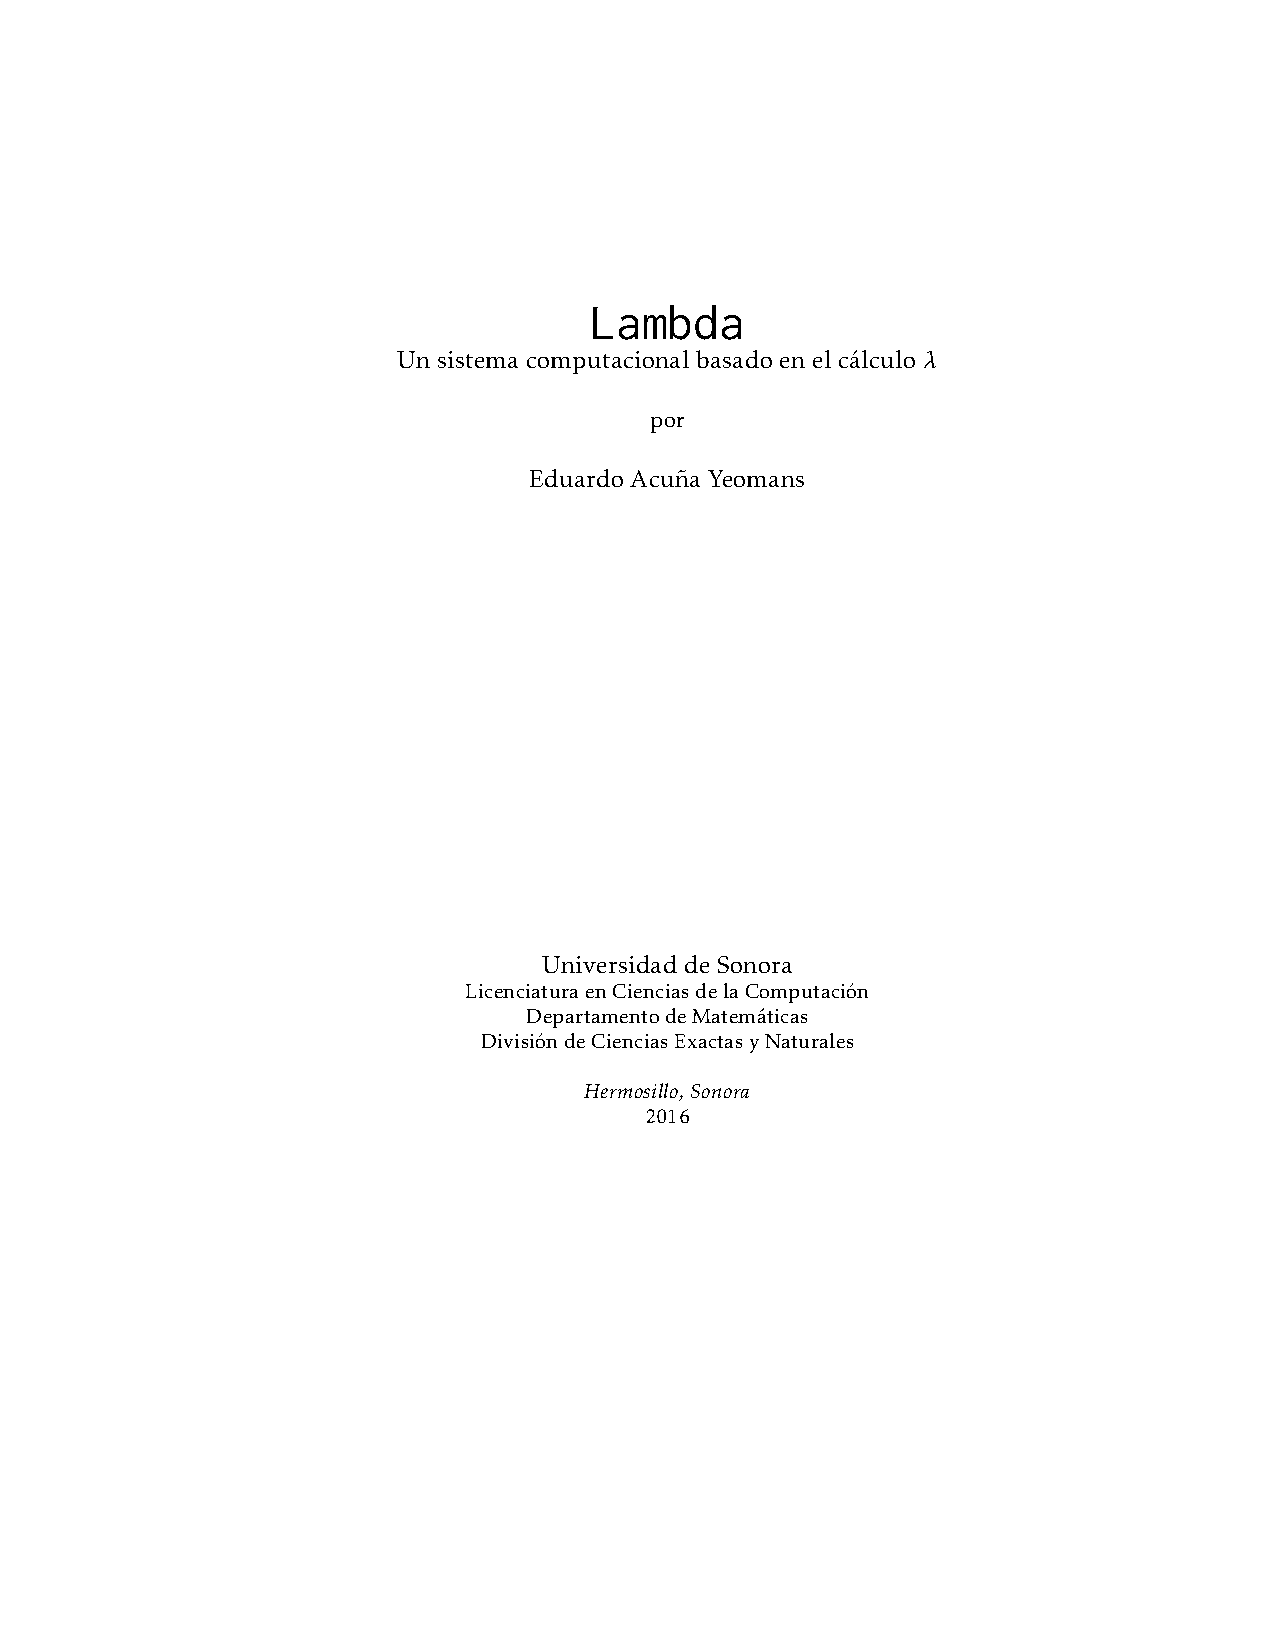
\includepdf[pages = -, pagecommand = {\thispagestyle{empty}}]{programas/lambda/main.pdf}

\nocite{*}
\bibliographystyle{acm}
\thispagestyle{empty}
{\small
\bibliography{bibliografia}}
\addcontentsline{toc}{chapter}{Bibliografía}

\end{document}


%%% Local Variables:
%%% mode: latex
%%% TeX-master: t
%%% End:
